\documentclass[a4paper]{article}
\usepackage[spanish]{babel}
\usepackage[utf8]{inputenc}
\usepackage{fancyhdr}
\usepackage{charter} % tipografia
%\usepackage{graphicx}
\usepackage[pdftex]{graphicx}
\usepackage{sidecap}
\usepackage{caption}
\usepackage{subcaption}
\usepackage{booktabs}
\usepackage{makeidx}
\usepackage{float}
\usepackage{amsmath, amsthm, amssymb}
\newtheorem{theorem}{Teorema}[section]
\newtheorem{corollary}{Corolario}[theorem]
\newtheorem{lemma}[theorem]{Lema}
\usepackage{amsfonts}
\usepackage{sectsty}
\usepackage{charter}
\usepackage{wrapfig}
\usepackage{listings}
\usepackage{hyperref} % links
\usepackage{algorithm} %http://www.ctan.org/pkg/algorithms
\usepackage{algorithmic}
\usepackage{color} % para snipets de codigo coloreados
\usepackage{fancybox} % para el sbox de los snipets de codigo
\definecolor{litegrey}{gray}{0.94}
% \newenvironment{sidebar}{%
% \begin{Sbox}\begin{minipage}{.85\textwidth}}%
% {\end{minipage}\end{Sbox}%
% \begin{center}\setlength{\fboxsep}{6pt}%
% \shadowbox{\TheSbox}\end{center}}
% \newenvironment{warning}{%
% \begin{Sbox}\begin{minipage}{.85\textwidth}\sffamily\lite\small\RaggedRight}%
% {\end{minipage}\end{Sbox}%
% \begin{center}\setlength{\fboxsep}{6pt}%
% \colorbox{litegrey}{\TheSbox}\end{center}}

%\newenvironment{codesnippet}{%
%\begin{Sbox}\begin{minipage}{\linewidth-2\fboxsep-2\fboxrule-4pt}\sffamily\small}%
%{\end{minipage}\end{Sbox}%
%\begin{center}%
%\colorbox{litegrey}{\TheSbox}\end{center}}

% \newenvironment{codesnippet}{\VerbatimEnvironment%
%   \noindent
%   %{\columnwidth-\leftmargin-\rightmargin-2\fboxsep-2\fboxrule-4pt}
%   \begin{Sbox}
%   \begin{minipage}{\linewidth-2\fboxsep-2\fboxrule-4pt}
%   \begin{Verbatim}
% }{%
%   \end{Verbatim}
%   \end{minipage}
%   \end{Sbox}%
%   \colorbox{litegrey}{\TheSbox}
% }

\newenvironment{codesnippet}{\VerbatimEnvironment%
  \noindent
  %      {\columnwidth-\leftmargin-\rightmargin-2\fboxsep-2\fboxrule-4pt}
  \begin{Sbox}
  \begin{minipage}{\linewidth}
  \begin{Verbatim}
}{%
  \end{Verbatim}
  \end{minipage}
  \end{Sbox}%
  \colorbox{litegrey}{\TheSbox}
}

\usepackage{fancyhdr}
\pagestyle{fancy}
%\renewcommand{\chaptermark}[1]{\markboth{#1}{}}
\renewcommand{\sectionmark}[1]{\markright{\thesection\ - #1}}
\fancyhf{}
\fancyhead[LO]{Sección \rightmark} % \thesection\
\fancyfoot[LO]{\small{Iv\'an Arcuschin, Mart\'in Jedwabny, Jos\'e Massigoge, Lucas Puterman}}
\fancyfoot[RO]{\thepage}
\renewcommand{\headrulewidth}{0.5pt}
\renewcommand{\footrulewidth}{0.5pt}
\setlength{\hoffset}{-0.8in}
\setlength{\textwidth}{16cm}
%\setlength{\hoffset}{-1.1cm}
%\setlength{\textwidth}{16cm}
\setlength{\headsep}{0.5cm}
\setlength{\textheight}{25cm}
\setlength{\voffset}{-0.7in}
\setlength{\headwidth}{\textwidth}
\setlength{\headheight}{13.1pt}
\renewcommand{\baselinestretch}{1.1} % line spacing
% \setcounter{secnumdepth}{2}
\usepackage{underscore}
\usepackage{caratula}
\usepackage{url}
\usepackage[usenames,dvipsnames]{xcolor}
\lstset{
    language=C++,
    basicstyle=\ttfamily,
    keywordstyle=\color{blue}\ttfamily,
    stringstyle=\color{red}\ttfamily,
    commentstyle=\color{ForestGreen}\ttfamily,
    morecomment=[l][\color{magenta}]{\#}
}

% *********************** %
% Ejercicio 2 - Agregado
% Grafos
\usepackage{tikz}
\usetikzlibrary{graphs}
\usetikzlibrary{calc}
\usetikzlibrary{arrows}
% Otros
\usepackage{arrayjobx}
\usepackage{enumitem}
\usepackage{multicol}
\usepackage{pgfplots}
% *********************** %

% ******************************************************** %
% TEMPLATE DE INFORME ORGA2 v0.1 %
% ******************************************************** %
% ******************************************************** %
% %
% ALGUNOS PAQUETES REQUERIDOS (EN UBUNTU): %
% ========================================
% %
% texlive-latex-base %
% texlive-latex-recommended %
% texlive-fonts-recommended %
% texlive-latex-extra %
% texlive-lang-spanish (en ubuntu 13.10) %
% ******************************************************** %
\begin{document}
\thispagestyle{empty}
\materia{Algoritmos y Estructura de Datos III}
\submateria{Primer Cuatrimestre de 2015}
\titulo{Trabajo Práctico III}
%\subtitulo{Grupo: }
\integrante{Iv\'an Arcuschin}{678/13}{iarcuschin@gmail.com}
\integrante{Mart\'in Jedwabny}{885/13}{martiniedva@gmail.com}
\integrante{Jos\'e Massigoge}{954/12}{jmmassigoge@gmail.com}
\integrante{Lucas Puterman}{830/13}{lucasputerman@gmail.com}
\maketitle
% no footer on the first page
\thispagestyle{empty}
\newpage

\tableofcontents

\newpage
\section{Ejercicio 1 - Demostración}
\subsection{Definiciones}

Sea G=(V,E) un grafo simple:

\begin{itemize}
\item Definición 1: D $\subseteq$ V es un \textbf{conjunto dominante} (CD) $\iff$ $\forall$ v $\in$ V, v $\in$ D ó $\exists$ w $\in$ D tal que (v,w) $\in$ E (tiene un vecino en D).
\item Definición 2: D $\subseteq$ V es un \textbf{conjunto independiente} (CI) $\iff$ $\forall$ v,w $\in$ D, (v,w) $\not\in$ E.
\item Definición 3: D $\subseteq$ V es un \textbf{conjunto independiente dominante} (CID) $\iff$ D es dominante e independiente.
\item Definición 4: D $\subseteq$ V es un \textbf{conjunto independiente dominante mínimo} (CIDM) $\iff$ D es el conjunto independiente dominante de V con menos nodos. Es decir que $\forall$ D' $\subseteq$ V tal que D' es independiente dominante, \#(D) $\leq$ \#(D').
\item Definición 5: D $\subseteq$ V es un \textbf{conjunto independiente maximal} (CIMax) $\iff$ D es independiente y $\not\exists$ D' $\subseteq$ V independiente tal que D $\subset$ D' ($\subset$ estricto).
\end{itemize}

\subsection{Ejercicio A}

\textit{Relacionar el problema de CIDM con el problema 3 del TP 1 (i.e., similitudes y diferencias):}

\medskip

Si definimos a G=(V,E) grafo simple para que represente al tablero de ajedrez que se forma en el ejercicio 3 del tp1, los nodos serían una cuadricula de la pinta (sin considerar los ejes, eso lo hacemos después):

\begin{figure}[h]
\begin{center}
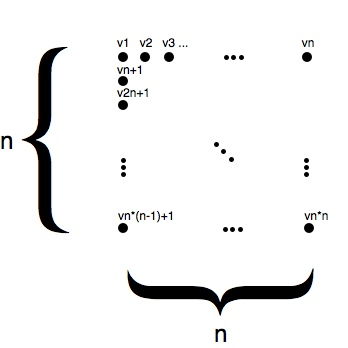
\includegraphics[scale=0.5]{imagenes/grafos-ej1-tp3-1.jpg}
\end{center}
\end{figure}

Donde 'n' es el parámetro del ejercicio que indica el tamaño de lado del tablero.

\newpage

Ahora, como el ejercicio consiste en poner la \underline{mínima} cantidad de \underline{caballos} para que todas las casillas tengan un caballo o bien estén amenazadas, podemos representar las 'amenazas' como los ejes del grafo, por ejemplo:

\begin{figure}[h]
\begin{center}
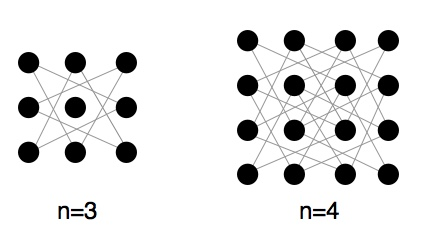
\includegraphics[scale=0.5]{imagenes/grafos-ej1-tp3-2.jpg}
\end{center}
\end{figure}

\textit{Observación: como cualquier posición x que amenaza a otra posicion 'y' sería amenazada si pongo un caballo en 'y', podemos representar el problema con un grafo simple y no un digrafo.}

\medskip

Entonces los ejercicios son similares ya que lo que estamos buscando en el ejercicio del TP1 es la mínima cantidad de caballos para que todas las posiciones (nodos) tengan un caballo o esten amenazadas (dominadas).

Es decir, si los caballos son un conjunto D de vértices en V, queremos hallar \#(D) tal que:
\begin{itemize}
\item $\forall$ v $\in$ V, v $\in$ D o $\exists$ w $\in$ D tal que (v,w) $\in$ E $\iff$ D es dominante.
\item $\forall$ D' $\subseteq$ V tal que D' es dominante, \#(D) $\leq$ \#(D') $\iff$ D es mínimo entre los conjuntos dominantes de V.
\end{itemize}

Por lo tanto el problema consiste en hallar un conjunto dominante mínimo pero, a diferencia del problema en este TP, puede o no ser independiente.
Esto se debe a que existen respuestas para el problema del TP1 donde hay caballos en ciertas posiciones que se amenazan entre sí:

\begin{figure}[h]
\begin{center}
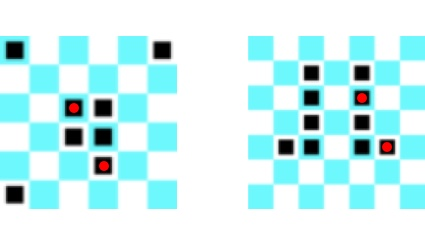
\includegraphics[scale=0.5]{imagenes/grafos-ej1-tp3-3.jpg}
\end{center}
\end{figure}

\textit{Observación: estos graficos fueron extraidos de la página: http://home.earthlink.net/~morgenstern/solution/knsols1.htm. El primero representa una solución óptima del ejercicio del TP1 con un tablero de 6x6 y la segunda imágen es para un tablero de 7x7. En ambas, se marcan con un punto negro los casilleros que tienen un caballo y, como vemos señalado en rojo, hay caballos en posiciones que se amenazan entre sí.}

\newpage

\subsection{Ejercicio B}

\textit{Demostrar que todo conjunto independiente maximal es un conjunto dominante:}

\medskip

Sea G=(V,E) un grafo simple y D $\subseteq$ V un conjunto independiente maximal, quiero ver que D es un conjunto dominante.\\
Supongamos (por absurdo) que D no es un conjunto dominante:
\begin{itemize}
\item[] $\Rightarrow$ $\exists$ v $\in$ V tal que v $\not\in$ D $\wedge$ $\forall$ w $\in$ D, (v,w) $\not\in$ E (no es vecino de ningún nodo en D).
\item[] $\Rightarrow$ D$\cup$\{v\} es independiente ya que como D es independiente sucede que $\forall$ w $\in$ D$\cup$\{v\} $\not\exists$ x $\in$ D tal que (x,w) $\in$ E.
\item[] $\Rightarrow$ Absurdo! pues D era maximal y $\exists$ D' = D$\cup$\{v\} tal que D' es independiente y D $\subset$ D', asi contradiciendo el hecho de que D es un conjunto independiente maximal.
\end{itemize}
Este absurdo vino de suponer que D no era dominante.\\
Por lo tanto, si D es un conjunto independiente maximal $\Rightarrow$ D es dominante.

\subsection{Ejercicio C}

\textit{Describir situaciones de la vida real que puedan modelarse utilizando CIDM:}

\medskip

\begin{itemize}
\item \textbf{El turista:} tenemos un conjunto de ciudades que forman un grafo simple conexo donde los nodos son las ciudades y dos nodos estan conectados si y solo si las ciudades son vecinas. Suponiendo que queremos conocer tantas culturas distintas como sea posible, decidimos que no queremos visitar ningun par de ciudades vecinas ya que sus culturas son muy similares. Como el problema que proponemos consiste en hallar un conjunto mínimo de ciudades (nodos en el mapa) tal que toda ciudad sea visitada o bien una ciudad vecina sea visitada pero no ambas (el conjunto de nodos sea independiente y dominante), podemos decir que estamos buscando un CIDM.
\item \textbf{Spamear una red social:} supongamos que tenemos un virus que se ocupa de spamear Facebook de manera que un mensaje sea propagado por toda la red. Asumimos que los usuarios de Facebook son nodos en un grafo simple conexo y que dos nodos estan conectados si y solo si esos dos usuarios son amigos en la red. Ahora, el virus no quiere ser descubierto, asi que lo que debe hacer es infectar la menor cantidad de cuentas que no sean amigas, ya que si spamea demasiadas cuentas o un par de cuentas que son amigas, sería mucho más fácil de descubrirlo. Luego, estamos buscando el mínimo conjunto de nodos en la red de usuarios tal que todos los usuarios vean el mensaje (dominación) y dos amigos no sean infectados a la vez (independencia), el cual es un CIDM.
\item \textbf{Cámaras de seguridad en un barrio:} tenemos casas en un barrio que representan los nodos de un grafo simple conexo, donde dos nodos estan conectados si y solo si sus casas respectivas con vecinas. Queremos poner cámaras de seguridad en el barrio de manera que toda casa tenga una cámara de seguridad o la tenga una casa vecina, ya que el rango de cobertura de la cámara es amplio y puede filmar la casa donde está y también las vecinas (dominación). No queremos poner cámaras en dos casas vecinas (independencia) para que no sea tan notorio y arruine el paisaje. A la vez, tenemos un presupuesto limitado, por lo cual queremos poner poner tan pocas cámaras como sea posible (minimalidad). Por lo tanto, el conjunto de casas que estamos buscando para ponerles cámaras es un CIDM.
\end{itemize}

\newpage
\section{Ejercicio 2 - Algoritmo exacto}
%\textit{Diseñar e implementar un algoritmo exacto para CIDM.}

\subsection{Ejercicio A}

\textit{Explicar detalladamente el algoritmo implementado. Elaborar podas y estrategias que permitan mejorar los tiempos de resolucion.}

\medskip

\subsubsection{Estrategia}
El algoritmo implementado se basa en la Técnica Algorítmica de \textit{Backtracking}.

En primer lugar notese que un conjunto dominante 'D' trivial es el conjunto de todos los nodos del grafo. Si bien este conjunto en principio no es independiente (a menos que $X(G) = \emptyset$), es el conjunto dominante más grande posible (no hay ningún nodo que quede afuera, es decir: $V(G) \setminus D = \emptyset$).

Luego, la idea principal del algorítmo es empezar con este primer conjunto dominante e ir sacando nodos recursivamente mientras chequeamos dominancia e independencia. Cada vez que encontramos un conjunto dominante e independiente, nos fijamos su cardinal. Si el cardinal de este nuevo conjunto es menor que el mínimo hasta ese momento nos quedamos con el nuevo y lo guardamos como mínimo. En caso de que el cardinal sea mayor, seguimos quitando nodos para encontrar un conjunto más chico.

\subsubsection{Podas}

Antes de mostrar cuales son las podas que utilizamos en el algoritmo, veamos algunos Lemas.

    \begin{lemma}
        Sea C un conjunto dominante e independiente de un grafo G. Entonces, cualquier subconjunto de C (distinto de C) es no-dominante respecto a G.
    \end{lemma}
    \begin{proof}[Demostración]
        Veamos que vale por absurdo. Supongamos H un subconjunto propio de C tal que $H \subset C$ y H es dominante de G. Como H está estrictamente incluido en C, entonces $\exists\ v \in C$ tal que $v \notin H$.

        Ahora, como C es independiente, no hay nodos de C que sean adyacentes en G, en particular: $\forall\ w \in C,\ (v,w) \notin X(G)$.

        Entonces, $v \in V(G)$ pero $v \notin H$ y $\forall\ w \in H \subset C,\ (v,w) \notin X(G)$. Luego, H no es dominante, ya que el nodo v no está en H ni tiene algún vecino que esté en H. Absurdo.
    \end{proof}

    \begin{lemma}
        Sea C un conjunto no-dominante respecto a G. Entonces, cualquier subconjunto de C es no-dominate respecto a G.
    \end{lemma}
    \begin{proof}[Demostración]
        Trivial. Sea H un subconjunto de C ($H \subseteq C$).

        Como C es no-dominante, $\exists\ v \in V(G)$ tal que $v \notin C$ y $\forall\ w \in C,\ (v,w) \notin X(G)$.

        Pero como $H \subseteq C$, $v \notin H$ y $\forall\ w \in H,\ (v,w) \notin X(G)$.

        Luego H es no-dominante respecto a G.
    \end{proof}

    Usando los resultados de estos dos lemas podemos optimizar el algortimo cortando ramas en el árbol de recursión.
    \begin{itemize}
        \item \textbf{Poda A}: por el primer Lema, cada vez que encontramos un conjunto dominante e independiente podemos ahí mismo devolver el que tenga menor cardinal entre ese conjunto y el mínimo encontrado hasta ese momento. Esto es así ya que sabemos que cualquier subconjunto del nuevo conjunto es no-dominante.
        \item \textbf{Poda B}: por el segundo Lema, al momento de sacar un nodo de un conjunto podemos chequear si el subconjunto es dominante o no. En caso de que no lo sea, ni siquiera lo procesamos, ya que no es dominante y ninguno de sus subconjuntos lo será.
    \end{itemize}
\subsubsection{Pseudocódigo}
\begin{codesnippet}
funcion resolver:
    Creamos un vector de n elementos, llenandolo con los nodos desde 0 a n-1.
    llamamos a resolver_aux pasandole como parametro la matriz de adyacencia, el vector
        recién creado y la cantidad de nodos en el grafo.

funcion resolver_aux:
    Llamemos dom al conjunto dominante pasado por parametro.
    Llamemos cidm al conjunto dominante e independiente con menor cardinal encontrado
        hasta ahora.
    Si el cidm tiene tamaño 1 hacer
        Devuelvo cidm
    Sino hacer
        // Chequeamos si dom es independiente:
        Para i desde 0 hasta |dom| hacer:
            Para j desde i+1 hasta |dom| hacer:
                Si matriz_adyacencia[dom[i]][dom[j]] == TRUE hacer
                    dom NO es independiente
        Si es independiente hacer
            Devolvemos el conjunto con menor cardinal entre cidm y dom.
    Para i desde 0 hasta |dom| hacer
        Crear un vector nuevo llamado copia con los mismos nodos que dom.
        Borrar el nodo en la posicion i del vector copia.
        // Chequeamos si el conjunto copia es dominante:
        Para i desde 0 hasta n hacer:
            Si i no pertenece a copia hacer
                Bool nodo_valido = FALSE
                Para j desde 0 hasta |copia| hacer:
                    Si copia[j] == i hacer
                        nodo_valido = TRUE
                    Si matriz_adyacencia[i][copia[j]] == TRUE hacer
                        nodo_valido = TRUE
                Si nodo_valido == FALSE hacer
                    copia NO es dominante
        Si copia es dominante hacer
            Hacer un llamado recursivo a resolver_aux, pasando como parametro la matriz
                de adyacencia, cidm, copia y la cantidad de nodos en el grafo.
            Llamemos nuevo_cidm al conjunto que devuelve el llamado recursivo.
            Devolvemos el conjunto con menor cardinal entre cidm y nuevo_cidm.
\end{codesnippet}

\subsection{Ejercicio B}

\textit{Calcular el orden de complejidad temporal de peor caso del algoritmo.}
\medskip

Veamos el costo de las distintas partes del algoritmo.

En la función \textit{resolver} tenemos un ciclo de $\Theta(n)$ más un llamado al constructor de la estructura vector para construir el primer conjunto dominante que se realiza solo una vez. Este constructor tiene costo $\Theta(n)$\footnote{Referencia: \url{http://www.cplusplus.com/reference/vector/vector/vector/}}, y dentro del ciclo solo tenemos operaciones constantes (asignación), por lo que el costo, sin contar el llamado a la función \textit{resolver_aux}, es de $\Theta(n)$.
En la función \textit{resolver_aux} tenemos 5 ciclos distintos, 2 anidados entre sí y otros 3 anidados entre sí.

Los primeros 2 corresponden al chequeo de indepedencia. Dentro de ellos solo hay operaciones de costo constante (una asignacion y dos comparaciones) y se repiten cada uno $|dom|$ veces, donde $dom$ es el conjunto dominante actual. Luego, el chequeo de independencia toma: $\mathcal{O}(|dom|*|dom|)$, que en el peor caso es $\mathcal{O}(n^2)$.

De los otros 3 ciclos anidados, el primero corresponde a la iteración sobre el conjunto $dom$ mientras vamos probando quitar distintos nodos, y los otros 2 corresponden al chequeo de dominancia de los nuevos conjuntos generados.
El primer ciclo se ejecuta $|dom|$ veces, mientras que el segundo y el tercero $n$ y $|copia|$ veces respectivamente, donde $copia$ es el nuevo conjunto generado (como se muestra en el pseudocódigo). Además dentro del primer ciclo utilizamos la función \textit{erase} de vectores que permite borrar un elemento dado su índice y el constructor de la estructura vector por copia. Ambas operaciones tiene costo en el peor caso lineal en la cantidad de elementos del vector original \footnote{Referencias: \url{http://www.cplusplus.com/reference/vector/vector/erase/} y \url{http://www.cplusplus.com/reference/vector/vector/vector/}}. El resto de las operaciones en los 3 ciclos es de costo constante (comparaciones y asignaciones).

Luego, la complejidad de los 3 ciclos nos queda: $\mathcal{O}(|dom|*(|dom| + |copia| + |n|* (|copia|)))$, que asintoticamente equivale a $\mathcal{O}(n^3)$

Fuera de los ciclos en la función \textit{resolver_aux} solo tenemos operaciones constantes (comparaciones y asignaciones, más la función \textit{size} de vectores, que tiene costo constante\footnote{Referencia: \url{http://www.cplusplus.com/reference/vector/vector/size/}}). Entonces, el costo de ejecutar una vez la función \textit{resolver_aux}, sin tener en cuenta el llamado recursivo a si misma, es de $\mathcal{O}(n^3)$.

Ahora, como vimos en el pseudocódigo, la función \textit{resolver_aux} parte del conjunto $dom$ y hace en el peor caso $|dom|$ llamados recursivos a si misma, cada uno quitando un nodo posible de $|dom|$.

Luego, el peor caso posible es que revisemos todas las posibles combinaciones de nodos. Es decir, pasar por \textit{resolver_aux} la cantidad de veces del cardinal del Conjunto de Partes de V(G). O sea, en el peor caso \textit{resolver_aux} toma: $\mathcal{O}(2^n*n^3)$.

Entonces, la complejidad final del algoritmo es:
$$\mathcal{O}(2^n*n^3)$$

%hablas de "los primeros dos ciclos", "los otros tres ciclos" y yo me quede como WTFF osea, no es que este mal, pero te hace volver al pseudocodigo y me marea, por ahi se entiende mas rapido si describis que hace cada ciclo cuando hablas de los ciclos

\subsection{Ejercicio C}

\textit{Realizar una experimentación que permita observar los tiempos de ejecución del algoritmo en función de los parámetros de la entrada y de las podas y/o estrategias implementadas.}
\medskip

Consideraciones:
\begin{itemize}
    \item Los casos de tests para esta experimentacion corresponden a grafos generados aleatoriamente, variando la cantidad de nodos y ejes.
    \item Los tiempos de ejecución se midieron con la biblioteca chrono y estos fueron convertidos a nanosegundos.
    \item Los valores aleatorios que fuimos tomando fueron generados con una distribución uniforme para el rango requerido.
    \item Los detalles de los parametros son:
        \begin{itemize}
            \item $2 \leq n \leq 9$
            \item $0 \leq m \leq n*(n-1)/2$
            \item Luego, para cada eje, se eligieron 2 nodos tales que $1 \leq v \leq n$, $1 \leq w \leq n$ y $(v,w) \notin X(G)$ donde $G$ es el grafo que estamos armando. Esto permite que el grafo tenga exactamente $m$ ejes (y no una cantidad menor que se podría dar al poner ejes que ya estaban).
        \end{itemize}
    \item Para cada caso de test, se midió la ejecución del algoritmo con y sin podas.
    \item Para cada $n$ se promediaron los resultados obtenidos para cada variaciones del algoritmo, con y sin podas.
\end{itemize}

Luego, queremos ver que el costo del algoritmo es, en el peor caso, el detallado en la sección Complejidad. La cota teórica calculada es $\mathcal{O}(2^n*n^3)$.

Los resultados obtenidos fueron los siguientes:

\begin{center}
    \begin{tikzpicture}
    \begin{axis}[
        title={},
        xlabel={$n$},
        ylabel={Tiempos de ejecucion (nanoseconds)},
        scaled x ticks=false,
        scaled y ticks=false,
        enlargelimits=0.05,
        width=0.5\textwidth,
        height=0.5\textwidth
    ]
    \addplot[color=black] table[x=n,y=sin-podas]{datos/datos-ej2.dat};
    \addplot[color=red] table[x=n,y=poda-A]{datos/datos-ej2.dat};
    \legend{Sin podas, Poda A}
    \end{axis}
    \end{tikzpicture}
    \begin{tikzpicture}
    \begin{axis}[
        title={},
        xlabel={$n$},
        ylabel={},
        scaled x ticks=false,
        scaled y ticks=false,
        enlargelimits=0.05,
        width=0.5\textwidth,
        height=0.5\textwidth
    ]
    \addplot[color=red] table[x=n,y=poda-A]{datos/datos-ej2.dat};
    \addplot[color=black] table[x=n,y=poda-B]{datos/datos-ej2.dat};
    \legend{Poda A,Poda B}
    \end{axis}
    \end{tikzpicture}

    \begin{tikzpicture}
    \begin{axis}[
        title={},
        xlabel={$n$},
        ylabel={Tiempos de ejecucion (nanoseconds)},
        scaled x ticks=false,
        scaled y ticks=false,
        enlargelimits=0.05,
        width=0.5\textwidth,
        height=0.5\textwidth
    ]
    \addplot[color=black] table[x=n,y=poda-B]{datos/datos-ej2.dat};
    \addplot[color=red] table[x=n,y=ambas-podas]{datos/datos-ej2.dat};
    \legend{Poda B, Ambas podas}
    \end{axis}
    \end{tikzpicture}
\end{center}

% Si luego dividimos por $2^n$, obtenemos:
%
% \begin{center}
%     \begin{tikzpicture}
%     \begin{axis}[
%         title={},
%         xlabel={$n$},
%         ylabel={Tiempos de ejecucion (nanoseconds)},
%         scaled x ticks=false,
%         scaled y ticks=false,
%         enlargelimits=0.05,
%         width=0.5\textwidth,
%         height=0.5\textwidth
%     ]
%     \addplot[color=black] table[x=n,y=sin-podas-div-2n]{datos/datos-ej2.dat};
%     \addplot[color=red] table[x=n,y=poda-A-div-2n]{datos/datos-ej2.dat};
%     \legend{sin-podas-div-2n, poda-A-div-2n}
%     \end{axis}
%     \end{tikzpicture}
%     \begin{tikzpicture}
%     \begin{axis}[
%         title={},
%         xlabel={$n$},
%         ylabel={},
%         scaled x ticks=false,
%         scaled y ticks=false,
%         enlargelimits=0.05,
%         width=0.5\textwidth,
%         height=0.5\textwidth
%     ]
%     \addplot[color=red] table[x=n,y=poda-A-div-2n]{datos/datos-ej2.dat};
%     \addplot[color=black] table[x=n,y=poda-B-div-2n]{datos/datos-ej2.dat};
%     \legend{poda-A-div-2n,poda-B-div-2n}
%     \end{axis}
%     \end{tikzpicture}
%
%     \begin{tikzpicture}
%     \begin{axis}[
%         title={},
%         xlabel={$n$},
%         ylabel={Tiempos de ejecucion (nanoseconds)},
%         scaled x ticks=false,
%         scaled y ticks=false,
%         enlargelimits=0.05,
%         width=0.5\textwidth,
%         height=0.5\textwidth
%     ]
%     \addplot[color=black] table[x=n,y=poda-B-div-2n]{datos/datos-ej2.dat};
%     \addplot[color=red] table[x=n,y=ambas-podas-div-2n]{datos/datos-ej2.dat};
%     \legend{poda-B-div-2n,ambas-podas-div-2n}
%     \end{axis}
%     \end{tikzpicture}
% \end{center}

Como se puede ver en los gráficos, los tiempos medidos tienen pinta exponencial, que se condice con la complejidad teórica calculada. Además, es claro que la poda B produce tiempos mucho mejores que la poda A, lo cual en principio no se esperaba.

Veamos que pasa cuando los dividimos por $2^n*n^3$:

\begin{center}
    \begin{tikzpicture}
    \begin{axis}[
        title={},
        xlabel={$n$},
        ylabel={Tiempos de ejecucion (nanoseconds)},
        scaled x ticks=false,
        scaled y ticks=false,
        enlargelimits=0.05,
        width=0.5\textwidth,
        height=0.5\textwidth
    ]
    \addplot[color=black] table[x=n,y=sin-podas-div-2nn3]{datos/datos-ej2.dat};
    \addplot[color=red] table[x=n,y=poda-A-div-2nn3]{datos/datos-ej2.dat};
    \legend{Sin podas, Poda A}
    \end{axis}
    \end{tikzpicture}
    \begin{tikzpicture}
    \begin{axis}[
        title={},
        xlabel={$n$},
        ylabel={},
        scaled x ticks=false,
        scaled y ticks=false,
        enlargelimits=0.05,
        width=0.5\textwidth,
        height=0.5\textwidth
    ]
    \addplot[color=red] table[x=n,y=poda-A-div-2nn3]{datos/datos-ej2.dat};
    \addplot[color=black] table[x=n,y=poda-B-div-2nn3]{datos/datos-ej2.dat};
    \legend{Poda A,Poda B}
    \end{axis}
    \end{tikzpicture}

    \begin{tikzpicture}
    \begin{axis}[
        title={},
        xlabel={$n$},
        ylabel={Tiempos de ejecucion (nanoseconds)},
        scaled x ticks=false,
        scaled y ticks=false,
        enlargelimits=0.05,
        width=0.5\textwidth,
        height=0.5\textwidth
    ]
    \addplot[color=black] table[x=n,y=poda-B-div-2nn3]{datos/datos-ej2.dat};
    \addplot[color=red] table[x=n,y=ambas-podas-div-2nn3]{datos/datos-ej2.dat};
    \legend{Poda B, Ambas podas}
    \end{axis}
    \end{tikzpicture}
\end{center}

Al realizar la división, podemos ver que los gráficos tienden a una constante arriba de cero, lo cual es lo esperado. Por lo tanto, el algoritmo tendría una complejidad $\mathcal{O}(c*2^n*n^3)$, donde $c$ es la constante a la cual converge el gráfico.


\newpage
\section{Ejercicio 3 - Heurística constructiva golosa}

\subsection{Ejercicio A}
Realizamos una heurística golosa para resolver el problema. Lo que hace el algoritmo es lo siguiente. Primero toma los datos de entrada del problema, y se arma la matriz o las listas de adyacencia del grafo (según la implementación elegida). Además, se crea un vector de nodos de tamaño $n$ donde cada nodo contiene guardado su número de nodo y el grado que tiene en el grafo. \\ 
Una vez que se procesaron los datos de entrada, se procede a resolver el problema. Para esto, se ordena el arreglo de nodos según sus grados de mayor a menor. Luego, se crea un arreglo de booleanos de tamaño n, donde cada uno está inicializado en $false$. En este arreglo se guarda si el nodo ya fue visitado o no. También se crea un arreglo llamado $cidm$ donde se guardará la solución. \\ 
Por último, se recorre en orden el arreglo de nodos ordenados según su grado. Si un nodo no fue visitado, se agrega el nodo a $cidm$ y luego se marcan como visitados a todos sus adyacentes (ya que queremos que sea dominante y mínimo).
Una vez que se recorre todo el arreglo, ya tenemos el $cidm$, solo resta mostrarlo por pantalla.

\subsection{Pseudocódigo}

\subsubsection{Implementación sobre listas de adyacencia}
\begin{codesnippet}
Crear listas de adyacencia con el input
Crear arreglo nodos que guarda numero de nodo y grado para cada nodo

Ordenar arreglo nodos segun su grado
Crear vector de booleanos visitado de tamano n para guardar nodos visitados
Crear vector cidm para guardar la solucion

Para cada nodo u en el arreglo ordenado:
	Si el nodo no fue visitado:
		agregar el nodo a cidm
		Para cada nodo w en su lista de adyacencia:
			marcar w como visitado
		fin Para
	fin Si
fin Para

mostrar cidm			
\end{codesnippet}

\subsubsection{Implementación sobre matriz de adyacencia}
\begin{codesnippet}
Crear matriz de adyacencia con el input
Crear arreglo nodos que guarda numero de nodo y grado para cada nodo

Ordenar arreglo nodos segun su grado
Crear vector de booleanos visitado de tamano n para guardar nodos visitados
Crear vector cidm para guardar la solucion

Para cada nodo u en el arreglo ordenado:
	Si el nodo no fue visitado:
		agregar el nodo a cidm
		Para cada nodo w en su fila de la matriz de adyacencia:
			Si el nodo w es adyacente:
				marcar w como visitado
			fin Si	
		fin Para
	fin Si
fin Para

mostrar cidm			
\end{codesnippet}



\subsection{Ejercicio B}
Calculemos la complejidad del algoritmo. Para esto vamos a calcular la complejidad para una implementación sobre matriz de adyacencia y una sobre listas de adyacencia. A su vez dividiremos el algoritmo en tres etapas, la entrada de datos, la resolución del problema y la salida de datos. \\ 


\begin{itemize}

\item Matriz de adyacencia

n la entrada de datos, se crea la matriz de adyacencia, esto tiene costo temporal $\mathcal{O}(n^2)$, a la vez, se crea el vector de Nodos, con costo $\mathcal{O}(n)$. Por lo tanto, la entrada de datos tiene costo $\mathcal{O}(n + n^2) \in \mathcal{O}(n^2)$. \\ 

La resolución del problema, comienza ordenando el arreglo de nodos, esto tiene costo  $\mathcal{O}(n*log(n)$. Luego, crea los vectores con costo constante. Por último, recorre todos los nodos ($n$), y por cada nodo, si no fue visitado, lo agrega a la solución con costo constante y se fija en su fila en la matriz de adyacencia quienes son sus vecinos y los marca como visitados. Esto tiene un costo de $\mathcal{O}(n^2)$. Por lo tanto todo el proceso tiene costo $\mathcal{O}(n*log(n) + n^2) \in \mathcal{O}(n^2)$.

Por último, se muestra el $cidm$ aproximado por pantalla, para eso se recorre el vector $cidm$ calculado en la resolución, que tiene a lo sumo tamaño $n$, por lo que tiene costo $\mathcal{O}(n)$. \\ 

Por lo tanto, juntando las tres etapas nos queda un costo total de  $\mathcal{O}(n^2 + n^2 + n) \in \mathcal{O}(n^2)$.\\ 

\item Listas de adyacencia

Primero se deben crear las listas de adyacencia, como tengo $m$ aristas y por cada una agrego en tiempo constante un elemento a 2 listas, esto tiene costo $\mathcal{O}(2m) \in  \mathcal{O}(m)$.

La resolución del problema, comienza ordenando el arreglo de nodos, esto tiene costo  $\mathcal{O}(n*log(n)$. Luego, tenemos $n$ listas pero la suma del tamaño de todas es de a lo sumo $2m$ , por lo tanto, se realizarán a lo sumo $2m$ operaciones en todo el ciclo, por lo que todo el proceso tiene costo $\mathcal{O}(n + 2m) \in \mathcal{O}(n + m)$. \\ 

Por último, se muestra el $cidm$ aproximado por pantalla, para eso se recorre el vector $cidm$ calculado en la resolución, que tiene a lo sumo tamaño $n$, por lo que tiene costo $\mathcal{O}(n)$. \\ 

Por lo tanto, juntando las tres etapas nos queda un costo total de  $\mathcal{O}(n*log(n) + n + m + n) \in \mathcal{O}(n*log(n) + m $

Entonces, la complejidad del algoritmo sobre listas de adyacencia es menor y es de:

$$ \mathcal{O}(n*log(n) + m)$$

\end{itemize}

\subsection{Ejercicio C}

Veamos un ejemplo de instancias donde la heurística golosa no funciona. Supongamos que tenemos un grafo $G$ con un nodo central $v$ y sean $w_i$ con $1 \leq i \leq k$ sus $k$ vecinos, y supongamos que todo $w_1$ tiene a su vez $k-2$ vecinos de grado 1, llamemoslos $u_{i,j}$ con $1 \leq i \leq k$ y $1 \leq j \leq k-2$. \\ 

\begin{figure}[H]
\centering
\begin{subfigure}[b]{0.5\textwidth}
                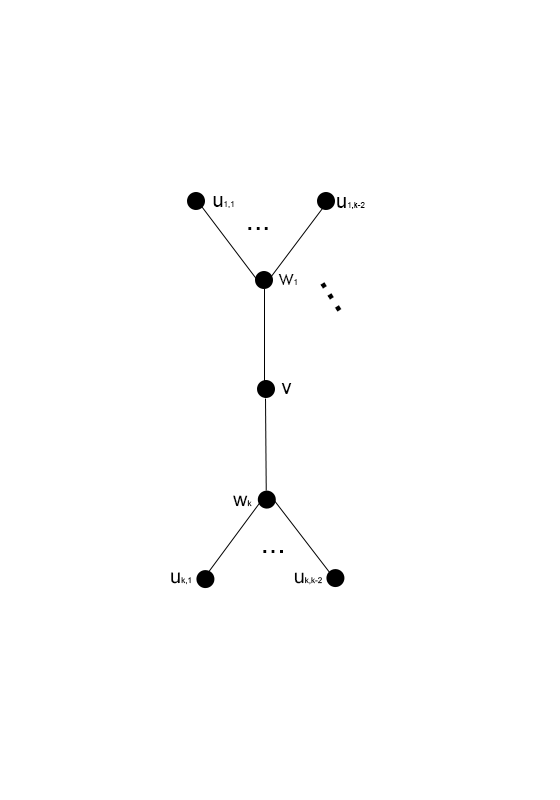
\includegraphics[width=\textwidth]{imagenes/grafos-ej3-tp3-1.png}
                \caption{}
        \end{subfigure}%
\end{figure}



 Ahora, al ordenar los nodos según su grado nos quedaría $v$ con $k$ vecinos, luego $w_i$ con $1 \leq i \leq k$, donde cada $w_i$ tiene grado $k-1$, y por último los $k * (k-2)$ nodos $u$ de grado 1. Al correr el algoritmo goloso, este arrojaría un DCIM con cardinalidad $k * (k-2) + 1$ ya que el algoritmo seleccionará a $v$ y a $u_{i,j}$ con $1 \leq i \leq k$ y $1 \leq j \leq k-2$. \\ 

\begin{figure}[H]
\centering
\begin{subfigure}[b]{0.5\textwidth}
                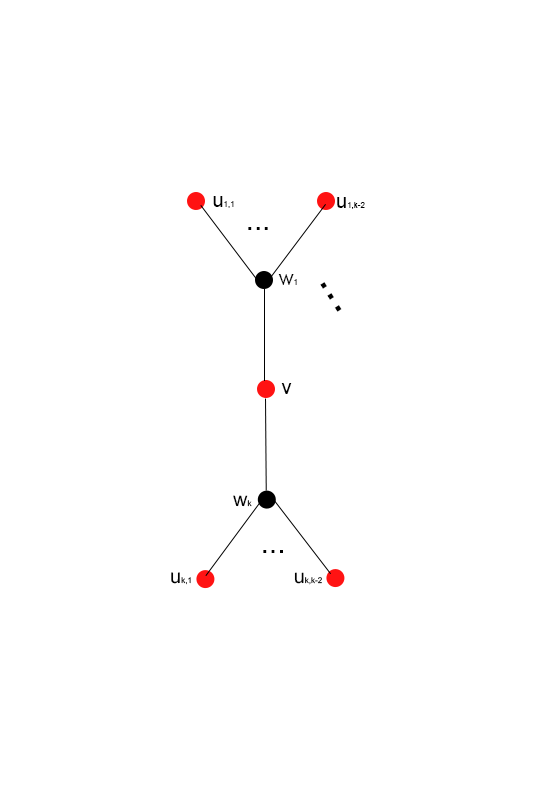
\includegraphics[width=\textwidth]{imagenes/grafos-ej3-tp3-2.png}
                \caption{}
        \end{subfigure}%
\end{figure}


 Sin embargo, si seleccionamos a todos los  $w_i$ con $1 \leq i \leq k$, tendríamos un DCIM real con cardinalidad $k$ que es mucho menor que el arrojado por el algoritmo.

\begin{figure}[H]
\centering
\begin{subfigure}[b]{0.5\textwidth}
                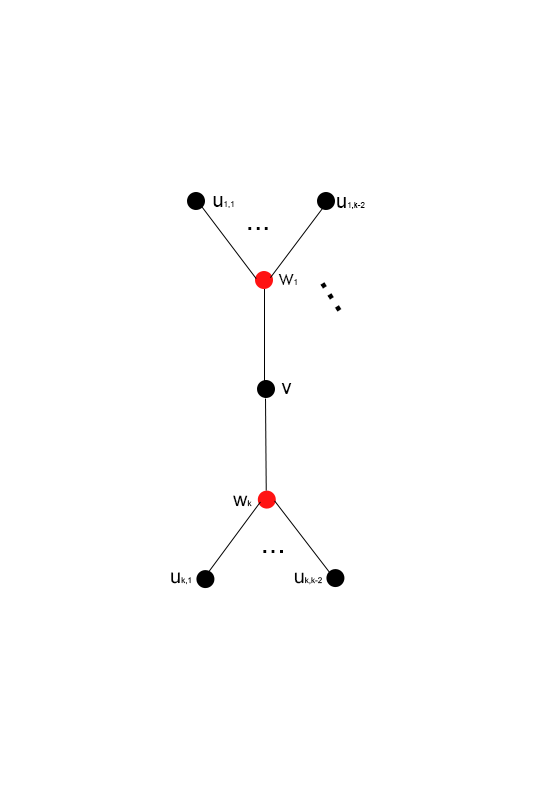
\includegraphics[width=\textwidth]{imagenes/grafos-ej3-tp3-3.png}
                \caption{}
        \end{subfigure}%
\end{figure}


Veamos que en este grafo $G=(V,E)$ tenemos $|V| = 1 + k*(k-1)$ nodos y nuestro algoritmo goloso arroja una solución de tamaño $1 + k*(k-2)$ es decir, solo quedan sin seleccionar $k$ nodos. Sin embargo, la solución optima sólo utiliza $k$ nodos. Notemos que el error es cuadrático.

\subsection{Ejercicio D}

Para la experimentación decidimos comparar distintas familias de instancias tanto en la implementación sobre matriz como el a de listas de adyacencia y comparar la eficiencia de ambas.

\subsubsection{Experimentación sobre grafo completo}

Se crearon instancias de grafos completos con $1 \leq n \leq 1000$.

En la implementación sobre matrices arrojo los siguientes resultados:\\ 

\begin{figure}[H]
        \centering
\begin{subfigure}[b]{0.5\textwidth}
                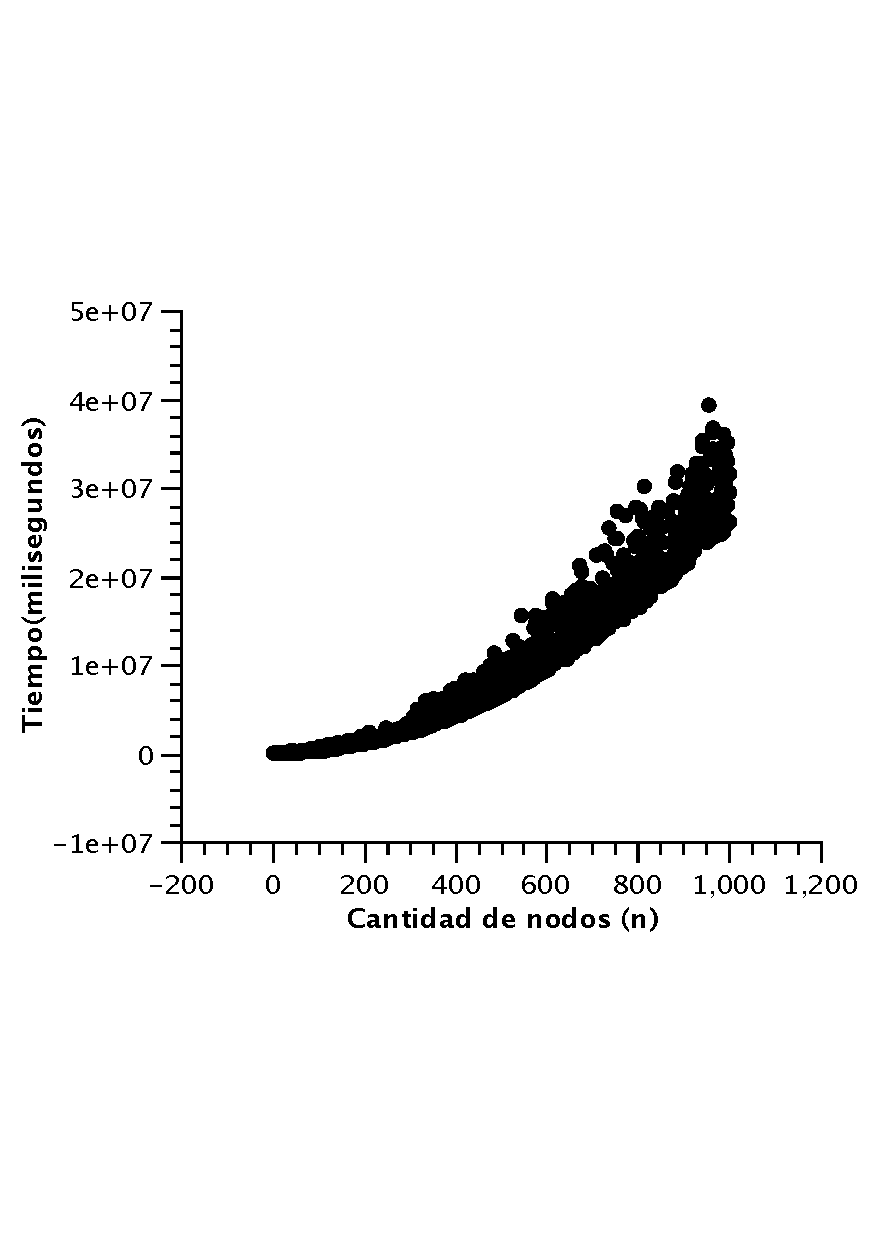
\includegraphics[width=\textwidth]{imagenes/completo-matriz-1.pdf}
                \caption{Tiempos sin procesar, en milisegundos}
        \end{subfigure}%

        \begin{subfigure}[b]{0.5\textwidth}
                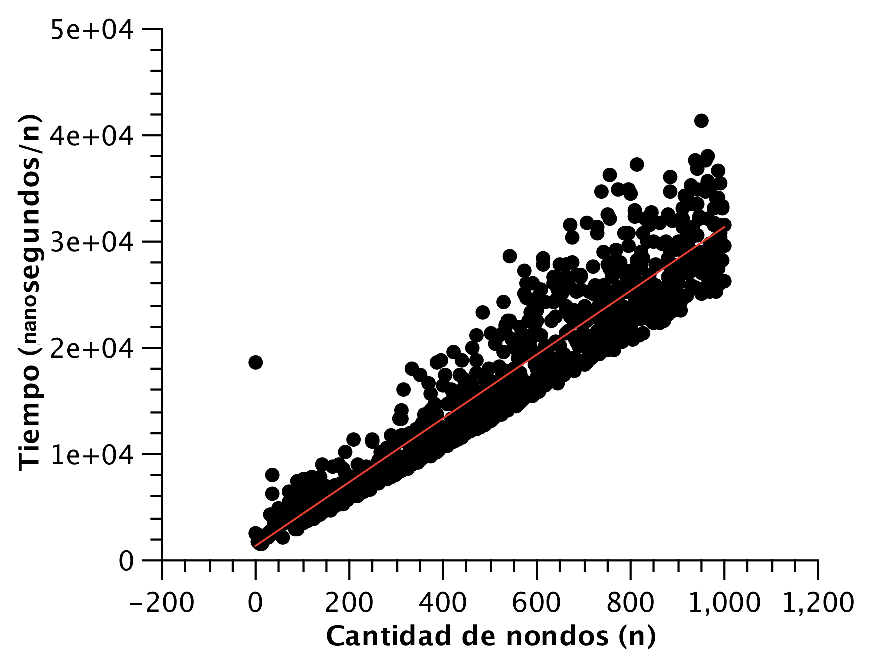
\includegraphics[width=\textwidth]{imagenes/completo-matriz-2.pdf}
                \caption{Dividiendo a los tiempos por $n$}
        \end{subfigure}

\end{figure}

\begin{figure}[H]
        \centering
        \begin{subfigure}[b]{0.5\textwidth}
                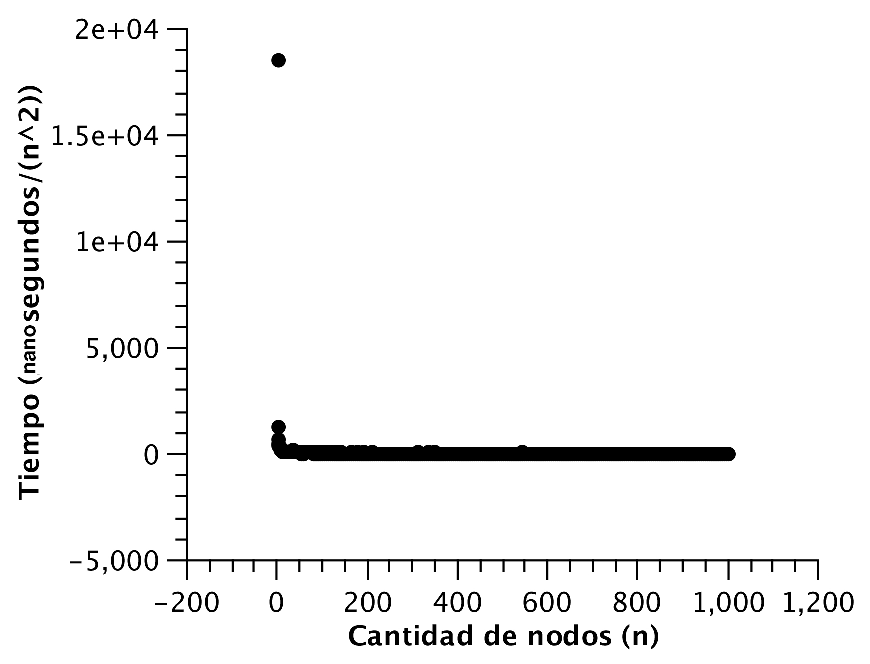
\includegraphics[width=\textwidth]{imagenes/completo-matriz-3.pdf}
                \caption{Dividiendo a los tiempos por $n^2$}
        \end{subfigure}

        \begin{subfigure}[b]{0.5\textwidth}
                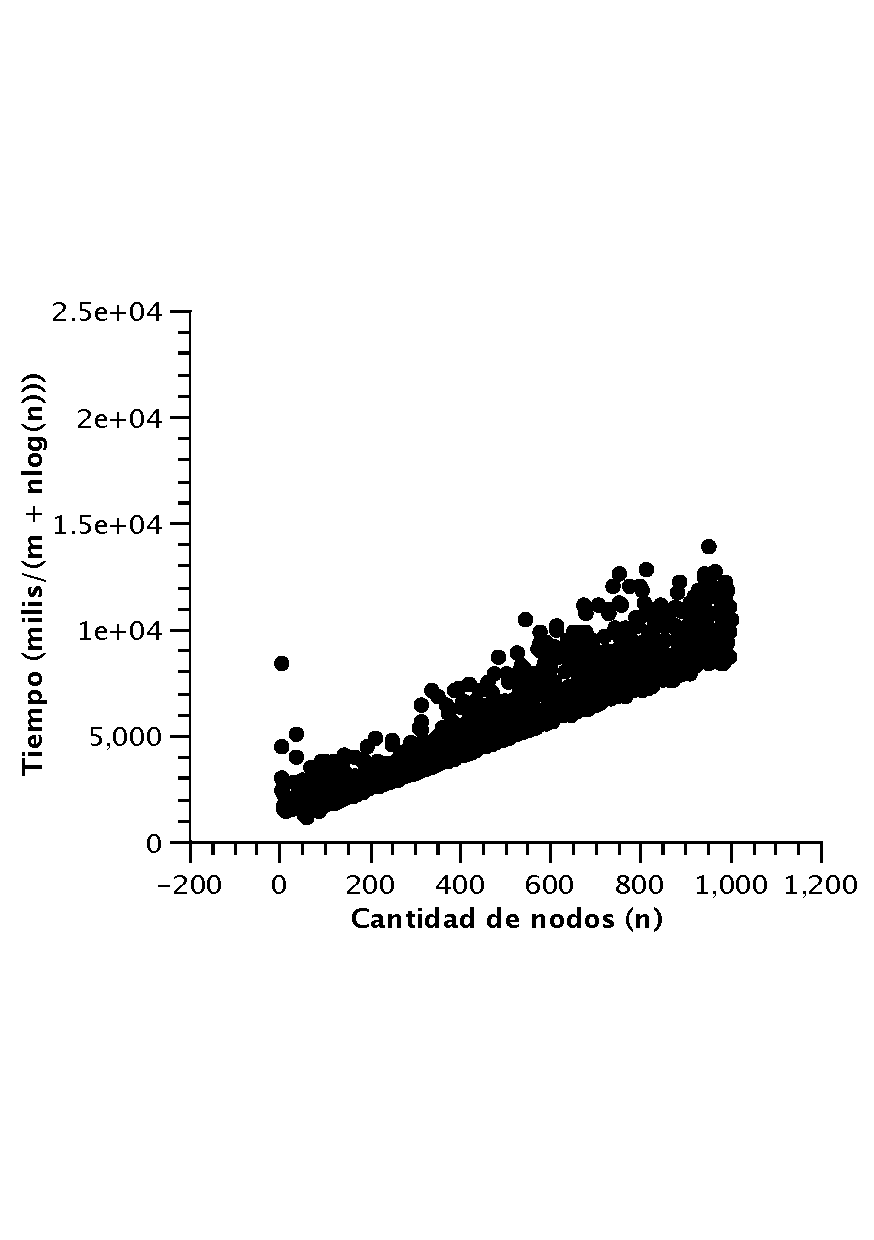
\includegraphics[width=\textwidth]{imagenes/completo-matriz-4.pdf}
                \caption{Dividiendo a los tiempos por $n + n*log(n)$}
        \end{subfigure}
\end{figure}

A continuación, adjuntamos una tabla con los últimos 20 valores obtenidos en las instancias, teniendo en cuenta que los casos fueron previamente ordenados según el tamaño ($n$):

\begin{table}[H]
\parbox{0.3\textwidth}{
    \begin{tabular}{ | l | l | l | l | l | l |}
    \hline
n   &Tiempo(milis) &m &Tiempo(mili/($n$)) &Tiempo(mili/($n^2$))) &Tiempo(mili/($n*log(n) + m$)))\\ \hline
980	&24,845,670	&479710	&25,352.72448979592	&25.870127030404	&8,475.696536553674\\ \hline
981	&33,412,818	&480690	&34,059.95718654434	&34.71963015957629	&11,384.934998666\\ \hline
982	&24,857,309	&481671	&25,312.94195519348	&25.77692663461658	&8,459.892640536484\\ \hline
983	&29,750,650	&482653	&30,265.15768056969	&30.78856325592033	&10,113.4891991821\\ \hline
984	&25,165,002	&483636	&25,574.18902439025	&25.99002949633155	&8,544.681225102551\\ \hline
985	&28,427,751	&484620	&28,860.66091370558	&29.3001633641681	&9,641.314760497822\\ \hline
986	&27,111,085	&485605	&27,496.02941176471	&27.88643956568429	&9,184.088121506702\\ \hline
987	&36,119,756	&486591	&36,595.49746707194	&37.07750503249436	&12,221.65041349897\\ \hline
988	&33,731,556	&487578	&34,141.25101214575	&34.5559220770706	&11,400.34121094489\\ \hline
989	&30,542,586	&488566	&30,882.29120323559	&31.22577472521294	&10,310.60678389385\\ \hline
990	&31,176,002	&489555	&31,490.91111111111	&31.80900112233446	&10,512.26503410799\\ \hline
991	&30,168,178	&490545	&30,442.15741675076	&30.71862504212993	&10,160.68392416765\\ \hline
992	&25,911,896	&491536	&26,120.86290322581	&26.33151502341311	&8,717.090324045907\\ \hline
993	&35,168,815	&492528	&35,416.73212487412	&35.6663969031965	&11,817.59489008868\\ \hline
994	&28,113,874	&493521	&28,283.5754527163	&28.45430126027797	&9,436.079245553556\\ \hline
995	&33,158,039	&494515	&33,324.66231155779	&33.49212292618873	&11,116.28719039287\\ \hline
996	&26,079,861	&495510	&26,184.59939759036	&26.28975843131563	&8,733.26701997587\\ \hline
997	&33,013,519	&496506	&33,112.85757271815	&33.21249505789183	&11,042.42206178822\\ \hline
998 &29,605,093	&497503	&29,664.42184368737	&29.72386958285308	&9,891.007222031083\\ \hline
999	&26,197,019	&498501	&26,223.24224224224	&26.24949173397622	&8,742.346964977023\\ \hline
1,000	&31,613,146	&499500	&31,613.146	&31.613146	&10,537.71533333333\\ \hline
    \end{tabular}
}
\end{table}

Como podemos ver la experimentación se condice con el cálculo teórico de la complejidad y arroja que es de $\mathcal{O}(n^2)$.

Veamos ahora los resultados en la implementación sobre listas de adyacencia:

\begin{figure}[H]
        \centering
\begin{subfigure}[b]{0.5\textwidth}
                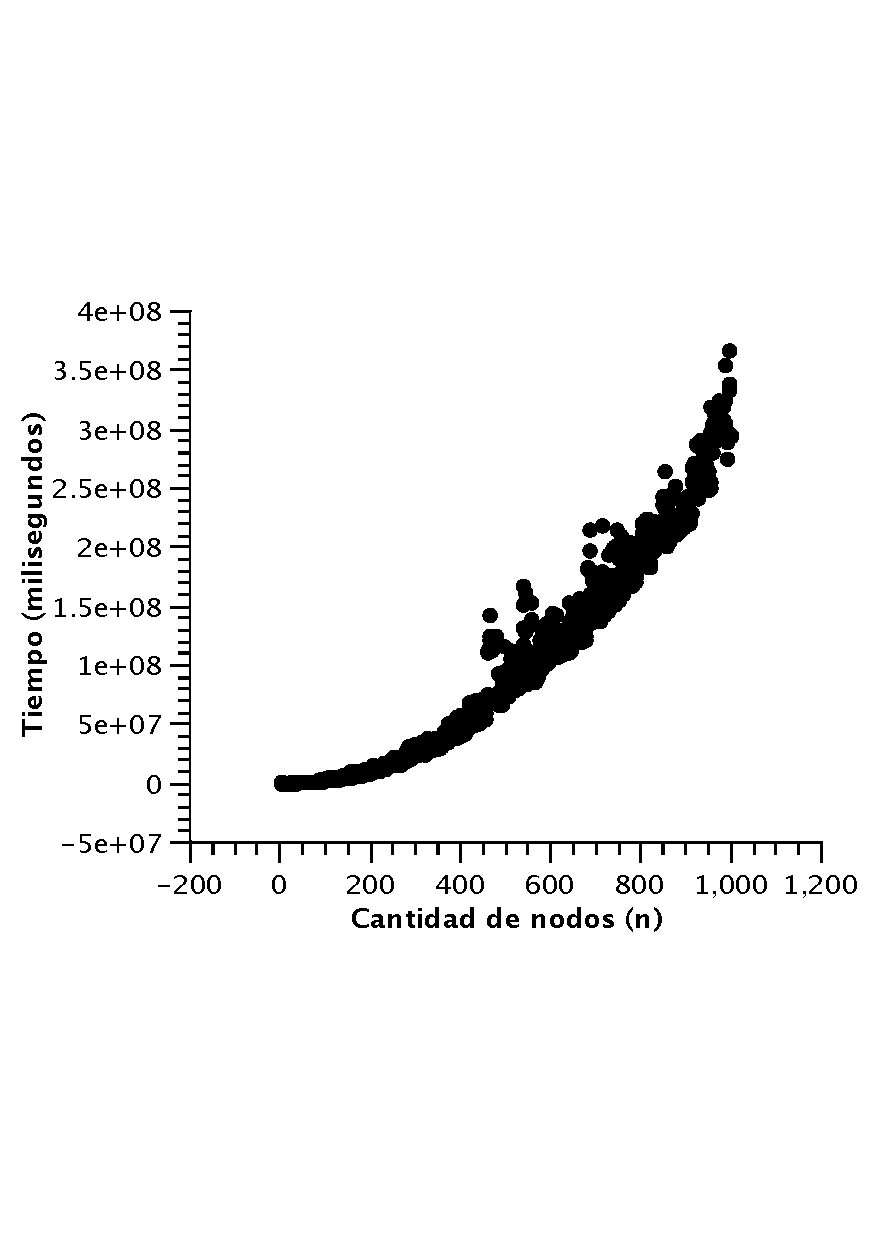
\includegraphics[width=\textwidth]{imagenes/completo-listas-1.pdf}
                \caption{Tiempos sin procesar, en milisegundos}
        \end{subfigure}%

        \begin{subfigure}[b]{0.5\textwidth}
                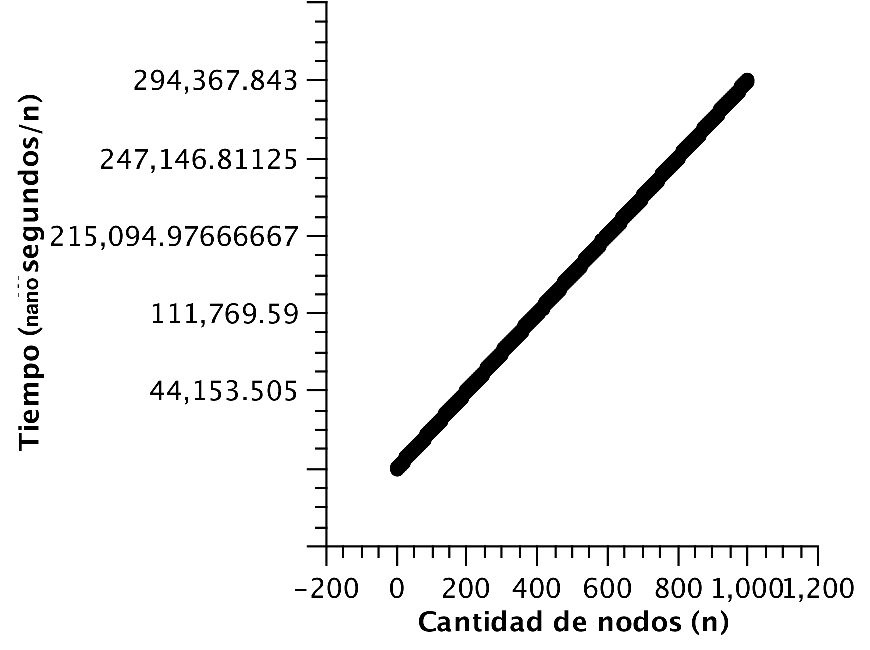
\includegraphics[width=\textwidth]{imagenes/completo-listas-2.pdf}
                \caption{Dividiendo a los tiempos por $n$}
        \end{subfigure}
\end{figure}

\begin{figure}[H]
        \centering
         \begin{subfigure}[b]{0.5\textwidth}
                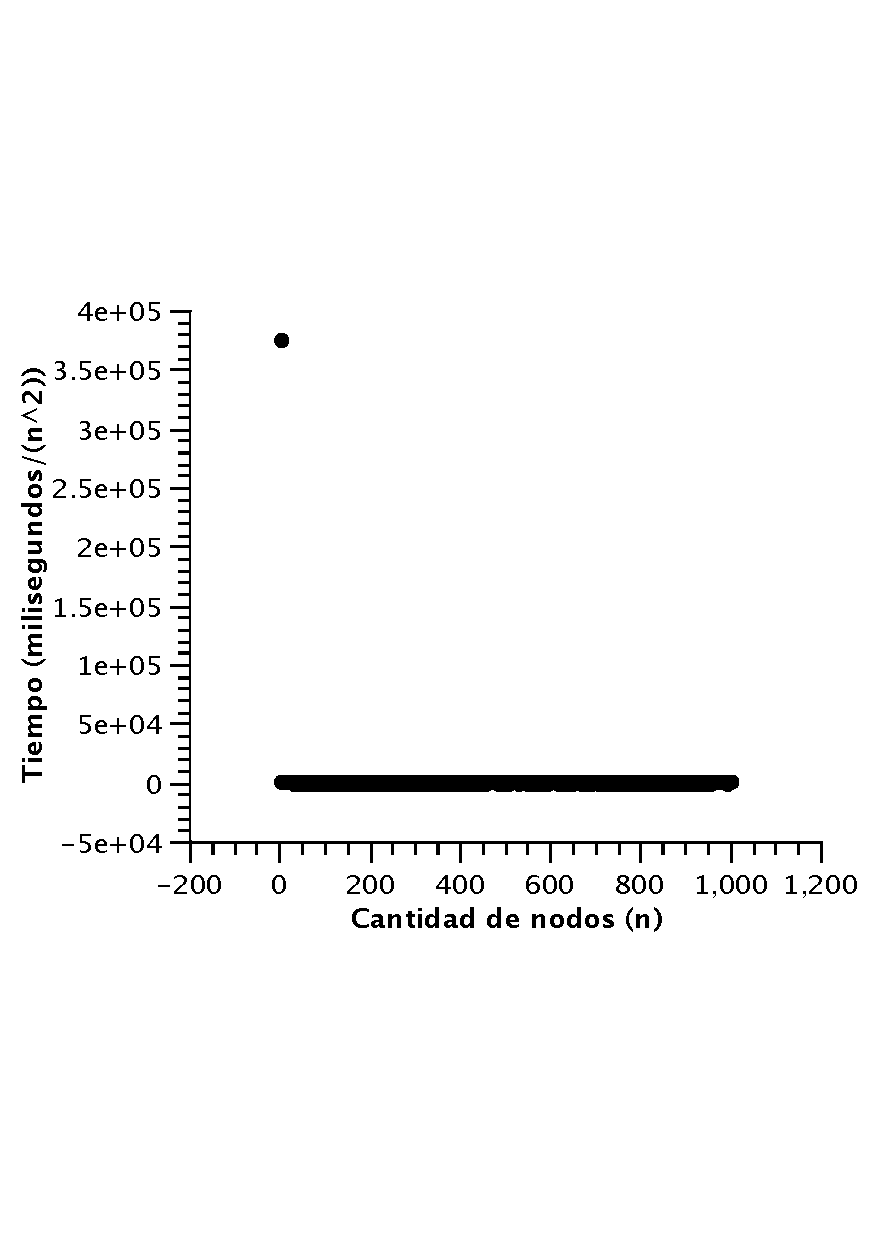
\includegraphics[width=\textwidth]{imagenes/completo-listas-3.pdf}
                \caption{Dividiendo a los tiempos por $n^2$}
        \end{subfigure}

        \begin{subfigure}[b]{0.5\textwidth}
                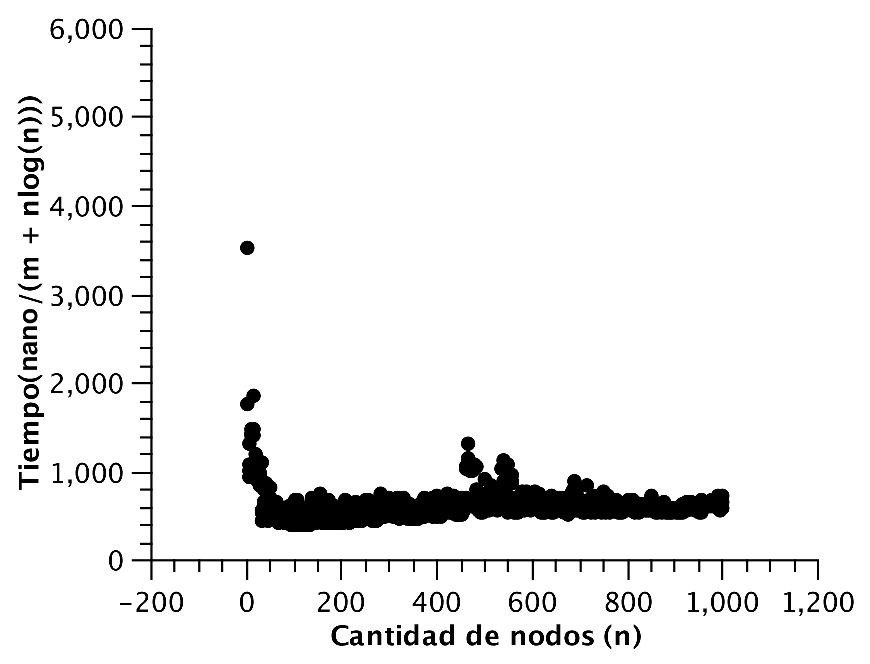
\includegraphics[width=\textwidth]{imagenes/completo-listas-4.pdf}
                \caption{Dividiendo a los tiempos por $n + n*log(n)$}
        \end{subfigure}
\end{figure}
A continuación, adjuntamos una tabla con los últimos 20 valores obtenidos en las instancias, teniendo en cuenta que los casos fueron previamente ordenados según el tamaño ($n$):

\begin{table}[H]
\parbox{0.3\textwidth}{
    \begin{tabular}{ | l | l | l | l | l | l |}
    \hline
n   &Tiempo(milis) &Tiempo(mili/($n$)) &Tiempo(mili/($n^2$))) &Tiempo(mili/($n*log(n) + m$))) &m\\ \hline
980	&296,879,716	&302,938.48571429	&309.1209037900875	&615.1144826034448	&479,710\\ \hline
981	&323,033,524	&329,290.03465851	&335.667721364436	&667.9423920520295	&480,690\\ \hline
982	&292,431,614	&297,791.86761711	&303.2503743555071	&603.4379490268261	&481,671\\ \hline
983	&297,273,430	&302,414.47609359	&307.6444314278647	&612.1842807953875	&482,653\\ \hline
984	&318,286,205	&323,461.59044715	&328.7211285032058	&654.1277503491588	&483,636\\ \hline
985	&308,937,975	&313,642.6142132	&318.4188976783736	&633.6298448756557	&484,620\\ \hline
986	&323,384,902	&327,976.57403651	&332.6334422276989	&661.9185207263685	&485,605\\ \hline
987	&304,973,689	&308,990.56636272	&313.0603509247369	&622.9719891480256	&486,591\\ \hline
988	&302,281,783	&305,953.22165992	&309.6692526922257	&616.2264905731232	&487,578\\ \hline
989	&353,599,216	&357,532.06875632	&361.5086640609904	&719.3873732062154	&488,566\\ \hline
990	&292,805,769	&295,763.4030303	&298.7509121518212	&594.5045184459034	&489,555\\ \hline
991	&289,577,857	&292,207.72653885	&294.8614798575678	&586.7671292958553	&490,545\\ \hline
992	&289,158,638	&291,490.5625	    &293.841292842742	&584.7394227940042	&491,536\\ \hline
993	&293,229,428	&295,296.50352467	&297.3781505787238	&591.7801781541916	&492,528\\ \hline
994	&275,111,868	&276,772.50301811	&278.443161990049	&554.102004459966	&493,521\\ \hline
995	&333,606,954	&335,283.37085427	&336.9682119138405	&670.5696612605566	&494,515\\ \hline
996	&338,319,005	&339,677.71586345	&341.041883397042	&678.679115312912	&495,510\\ \hline
997	&332,699,588	&333,700.69007021	&334.7048044836616	&666.0709764219323	&496,506\\ \hline
998	&366,440,239	&367,174.58817635	&367.9104089943414	&732.1539875453961	&497,503\\ \hline
999	&296,662,430	&296,959.38938939	&297.2566460354248	&591.5530805302149	&498,501\\ \hline
1,000	&294,367,843	&294,367.843    &294.367843         &585.8066527363184  &499,500\\ \hline
    \end{tabular}
}
\end{table}

Como podemos ver, la experimentación se condice con el cálculo teórico de la complejidad y arroja que es de $\mathcal{O}(n*log(n) + m)$, aunque en un grafo completo es casi $\mathcal{O}(n^2)$.



\subsubsection{Experimentación sobre el complemento del grafo completo}

Se crearon instancias de complementos grafos completos con $1 \leq n \leq 1000$ y $m = 0$.

En la implementación sobre matrices arrojo los siguientes resultados:\\ 

\begin{figure}[H]
        \centering
\begin{subfigure}[b]{0.5\textwidth}
                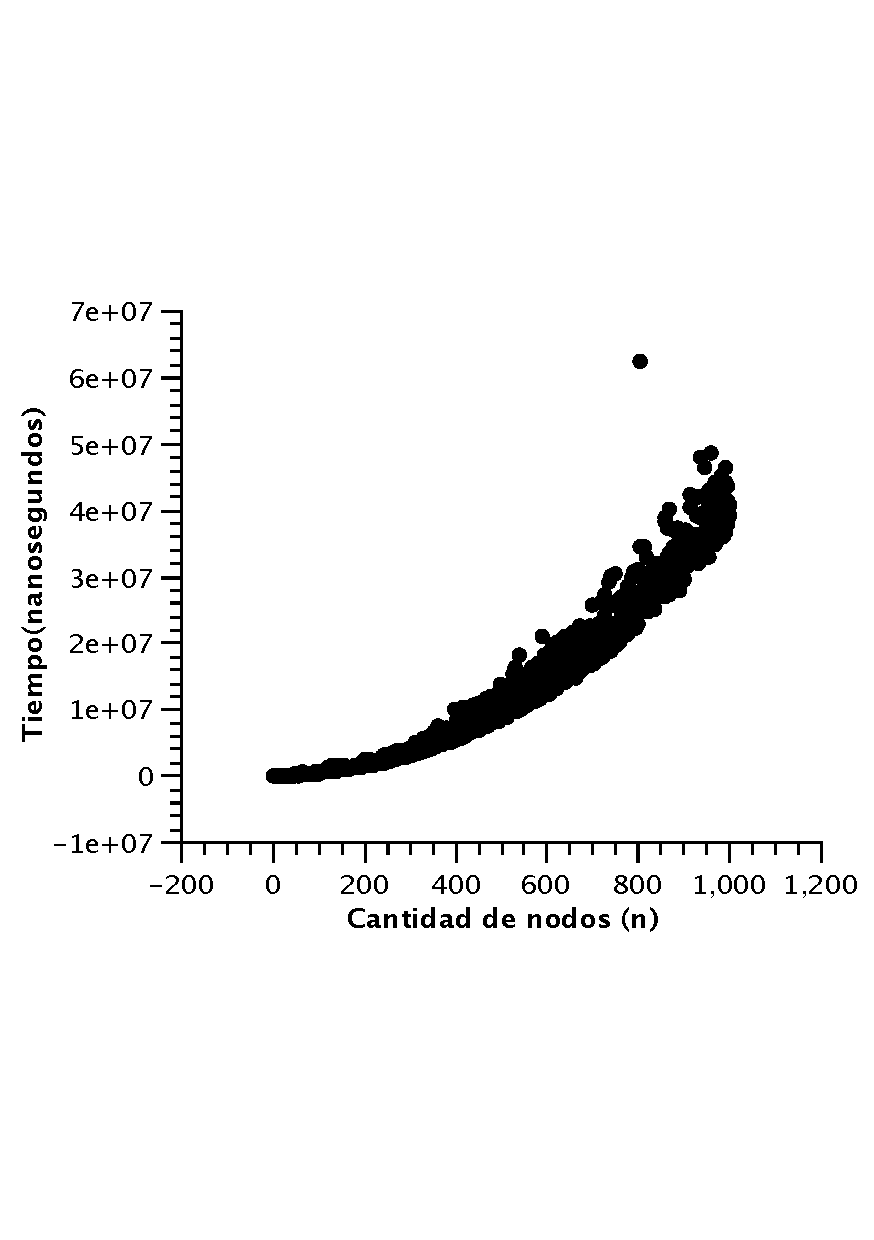
\includegraphics[width=\textwidth]{imagenes/vacio-matriz-1.pdf}
                \caption{Tiempos sin procesar, en milisegundos}
        \end{subfigure}%

        \begin{subfigure}[b]{0.5\textwidth}
                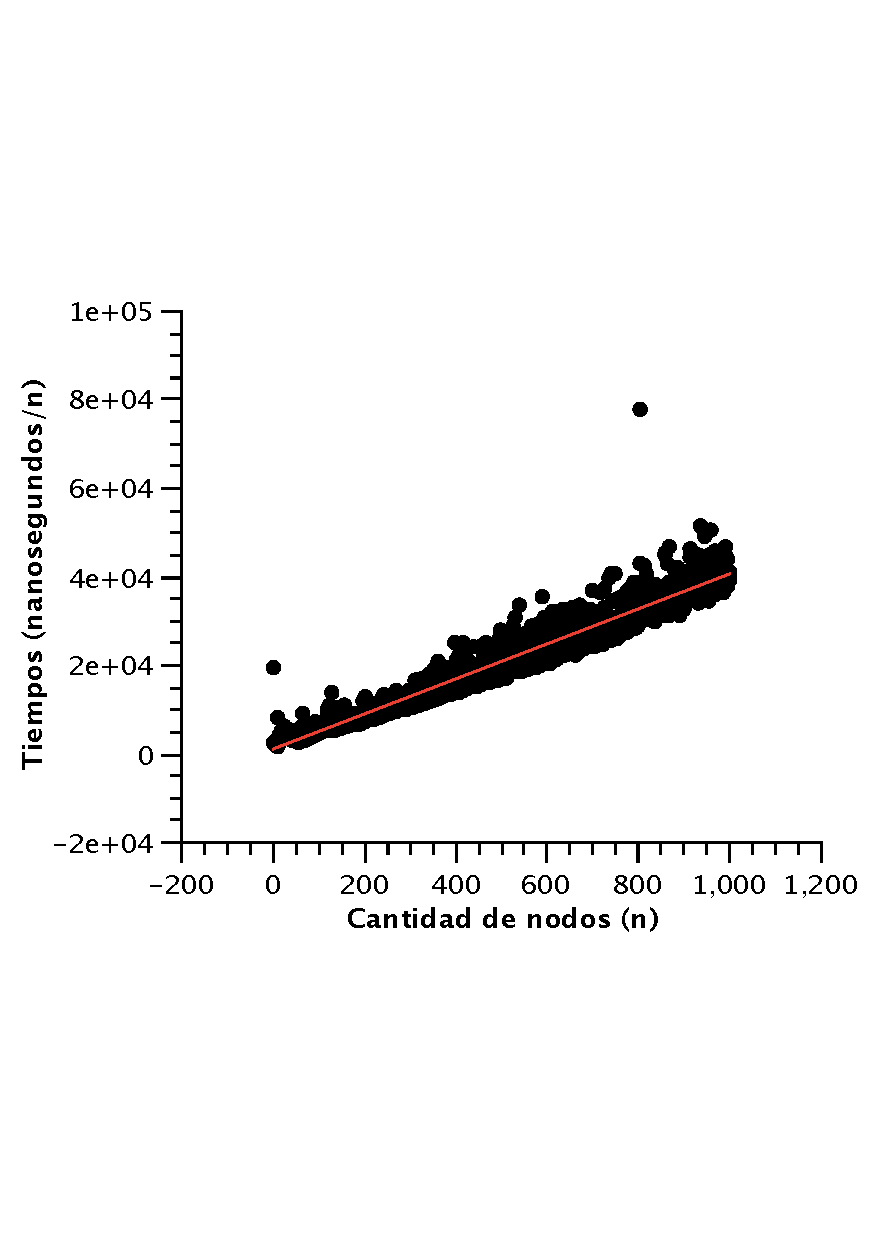
\includegraphics[width=\textwidth]{imagenes/vacio-matriz-2.pdf}
                \caption{Dividiendo a los tiempos por $n$}
        \end{subfigure}



\end{figure}

\begin{figure}[H]
        \centering
        \begin{subfigure}[b]{0.5\textwidth}
                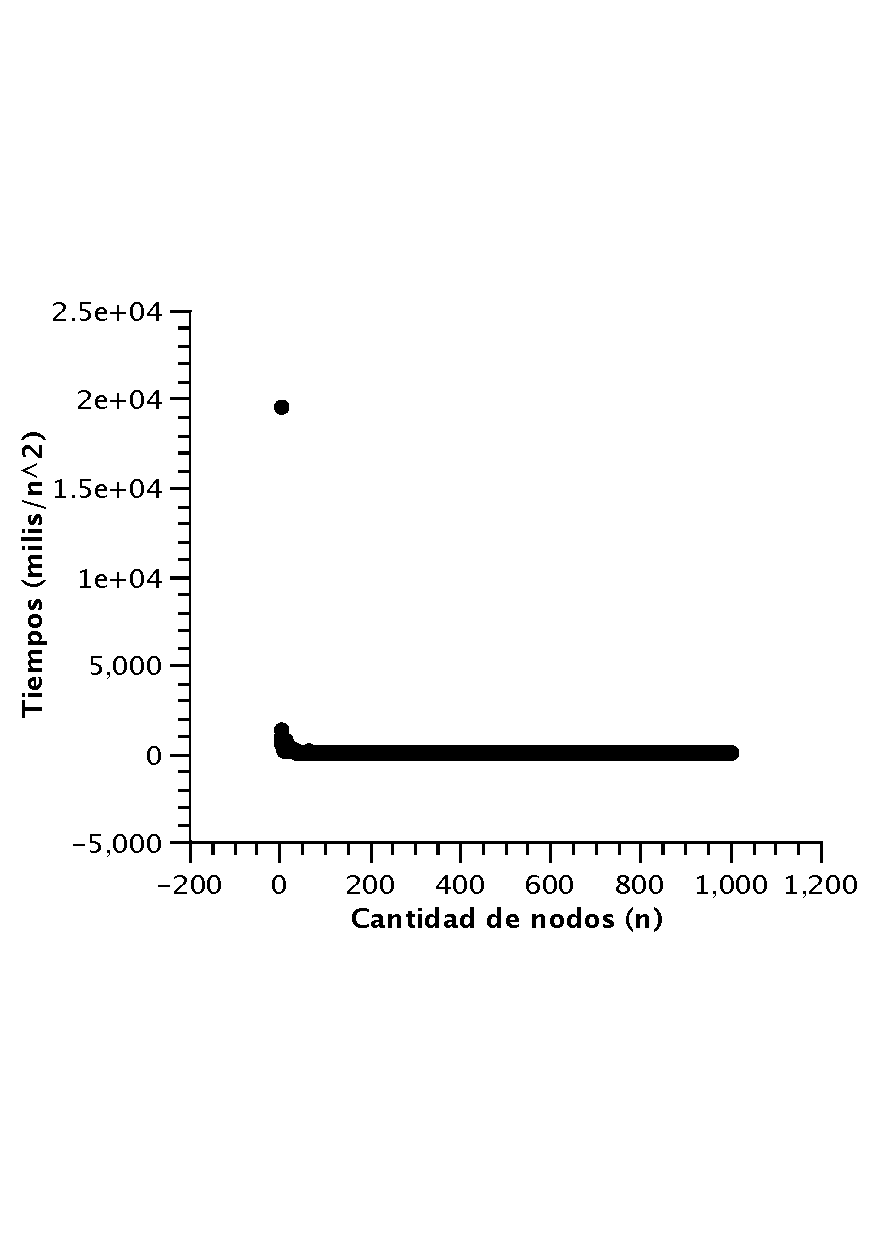
\includegraphics[width=\textwidth]{imagenes/vacio-matriz-3.pdf}
                \caption{Dividiendo a los tiempos por $n^2$}
        \end{subfigure}

        \begin{subfigure}[b]{0.5\textwidth}
                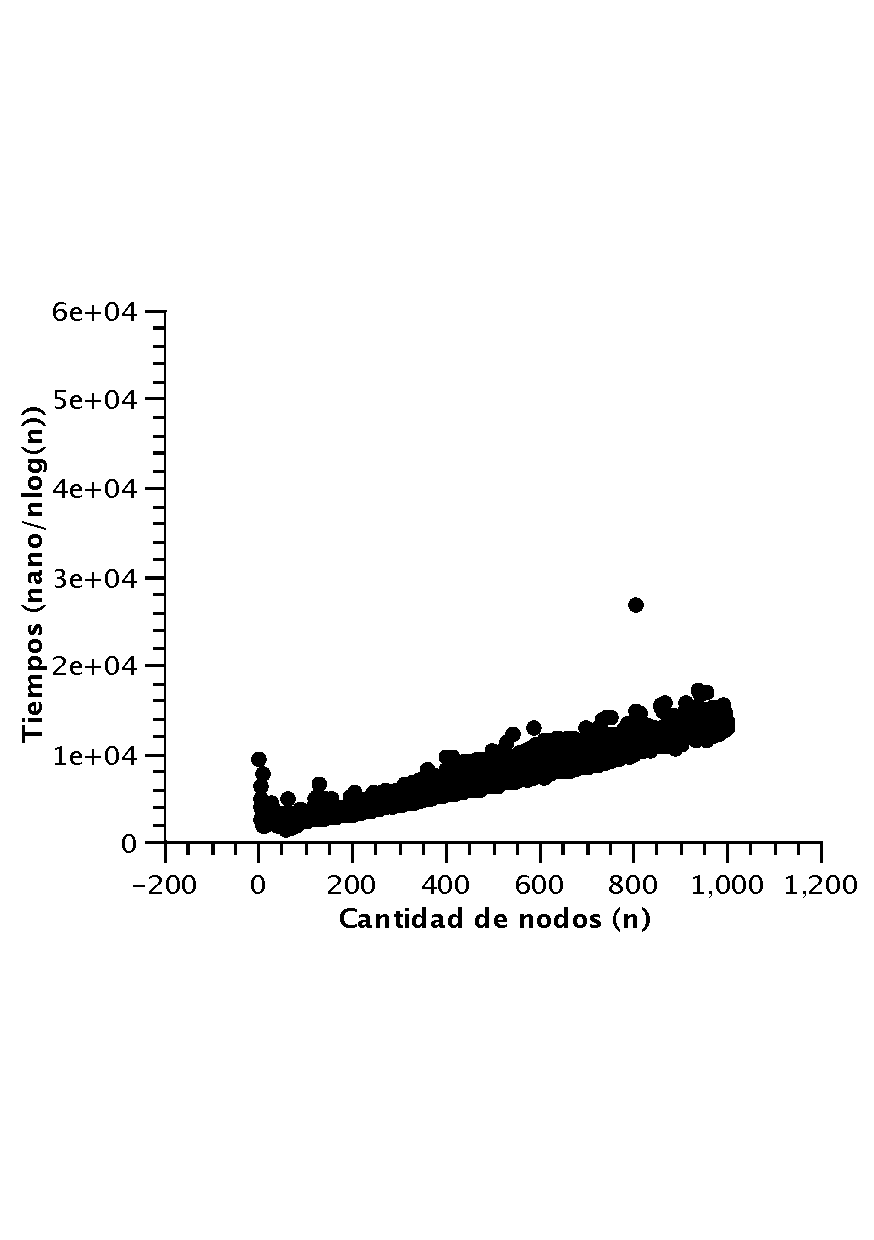
\includegraphics[width=\textwidth]{imagenes/vacio-matriz-4.pdf}
                \caption{Dividiendo a los tiempos por $n + n*log(n)$}
        \end{subfigure}
\end{figure}

A continuación, adjuntamos una tabla con los últimos 20 valores obtenidos en las instancias, teniendo en cuenta que los casos fueron previamente ordenados según el tamaño ($n$):

\begin{table}[H]
\parbox{0.3\textwidth}{
    \begin{tabular}{ | l | l | l | l | l |}
    \hline
n   &Tiempo(milis) &Tiempo(mili/($n$)) &Tiempo(mili/($n^2$))) &Tiempo(mili/($n*log(n) + m$)))\\ \hline
980	&41,753,937	&42,606.0581632653	&43.47556955435235	&14,243.67703581269\\ \hline
981	&37,549,011	&38,276.25993883792	&39.01759422919258	&12,794.28300537819\\ \hline
982	&39,391,112	&40,113.14867617108	&40.84842024050008	&13,406.30148305065\\ \hline
983	&45,239,903	&46,022.28179043744	&46.81819103808488	&15,378.93358170479\\ \hline
984	&36,000,279	&36,585.6493902439	&37.18053799821535	&12,223.75853853513\\ \hline
985	&43,702,767	&44,368.29137055838	&45.0439506300085	&14,821.85954673998\\ \hline
986	&40,825,343	&41,405.01318458418	&41.99291398030849	&13,829.89827602756\\ \hline
987	&38,862,643	&39,374.5116514691	&39.89312224059685	&13,149.74655118415\\ \hline
988	&36,831,350	&37,278.6943319838	&37.73147199593502	&12,447.98660517573\\ \hline
989	&44,397,040	&44,890.83923154702	&45.39013066890497	&14,987.61178273532\\ \hline
990	&39,102,722	&39,497.69898989899	&39.89666564636262	&13,185.08310395429\\ \hline
991	&40,118,814	&40,483.16246215944	&40.85081984072598	&13,512.07184160979\\ \hline
992	&46,471,583	&46,846.35383064516	&47.22414700669875	&15,633.62968546942\\ \hline
993	&41,389,046	&41,680.81168177241	&41.97463412061673	&13,907.7469205387\\ \hline
994	&43,743,891	&44,007.93863179074	&44.27358011246553	&14,682.10400263076\\ \hline
995	&38,823,308	&39,018.4	        &39.21447236180904	&13,015.57795408459\\ \hline
996	&37,960,325	&38,112.77610441767	&38.26583946226674	&12,711.63425257771\\ \hline
997	&39,036,157	&39,153.61785356068	&39.27143215001071	&13,056.88500714597\\ \hline
998	&40,876,628	&40,958.54509018036	&41.0406263428661	&13,656.80637315606\\ \hline
999	&40,732,820	&40,773.59359359359	&40.81440800159519	&13,593.16666151807\\ \hline
    \end{tabular}
}
\end{table}

Como podemos ver, la experimentación se condice con el cálculo teórico de la complejidad y, aunque el no haya aristas en el grafo, la complejidad que arroja es de $\mathcal{O}(n^2)$.


Veamos ahora los resultados en la implementación sobre listas de adyacencia:

\begin{figure}[H]
        \centering
\begin{subfigure}[b]{0.5\textwidth}
                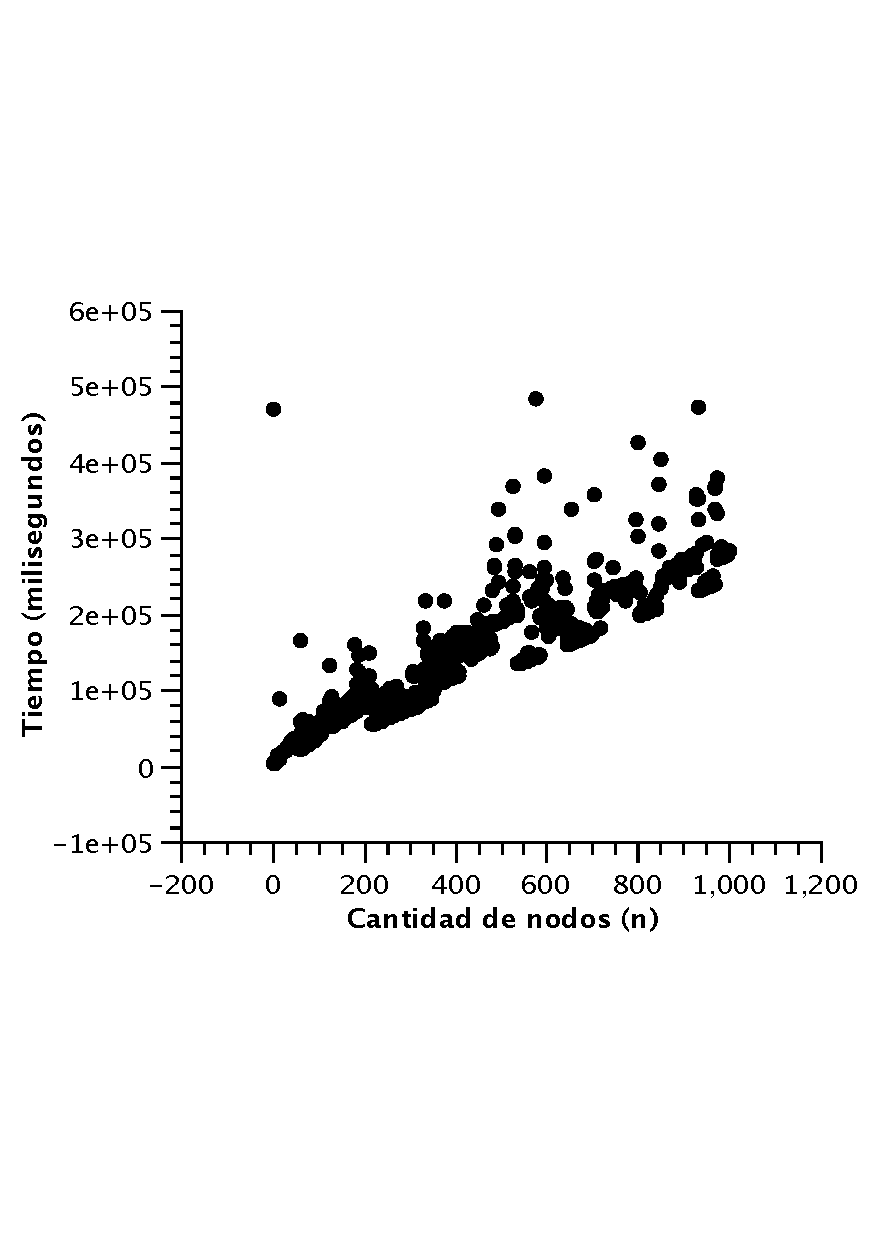
\includegraphics[width=\textwidth]{imagenes/vacio-listas-1.pdf}
                \caption{Tiempos sin procesar, en milisegundos}
        \end{subfigure}%

        \begin{subfigure}[b]{0.5\textwidth}
                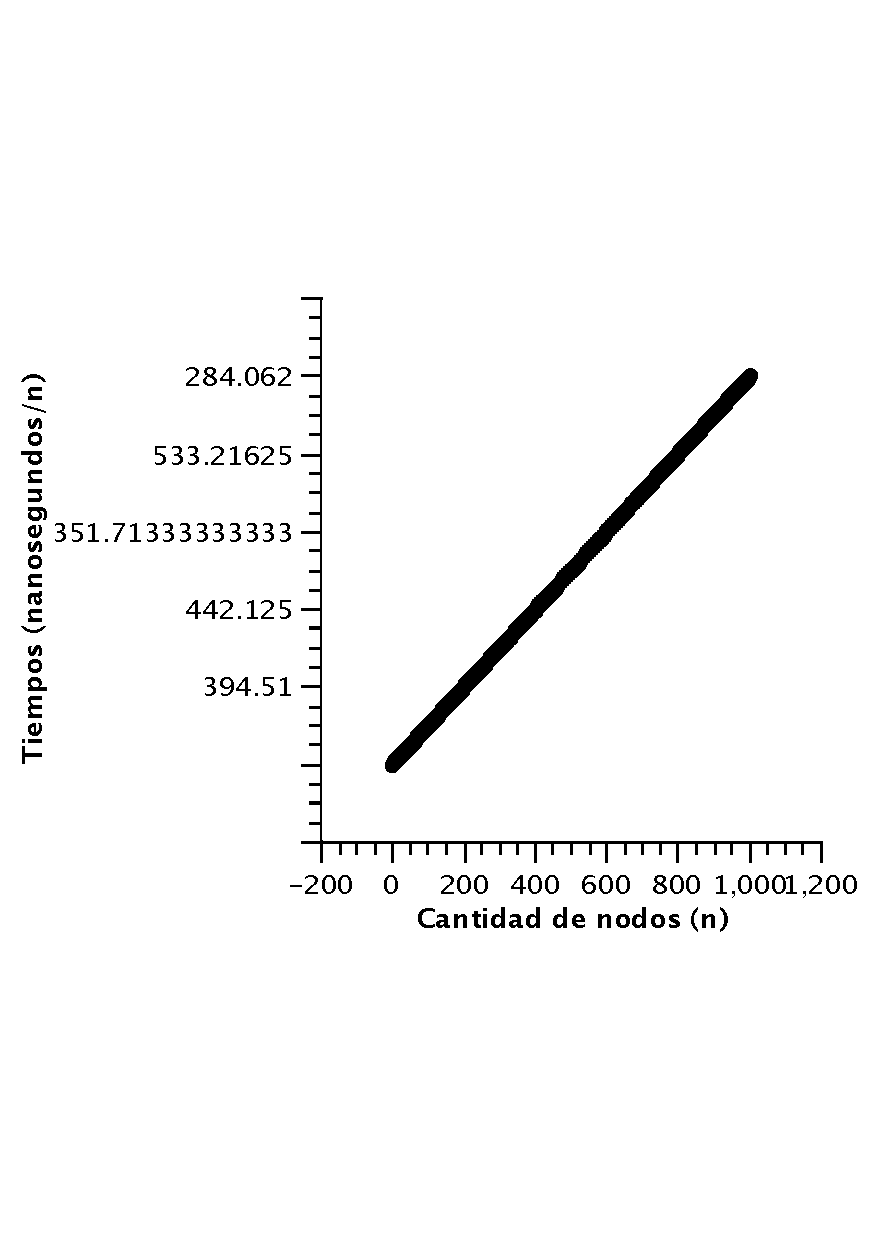
\includegraphics[width=\textwidth]{imagenes/vacio-listas-2.pdf}
                \caption{Dividiendo a los tiempos por $n$}
        \end{subfigure}


\end{figure}

\begin{figure}[H]
        \centering
        \begin{subfigure}[b]{0.5\textwidth}
                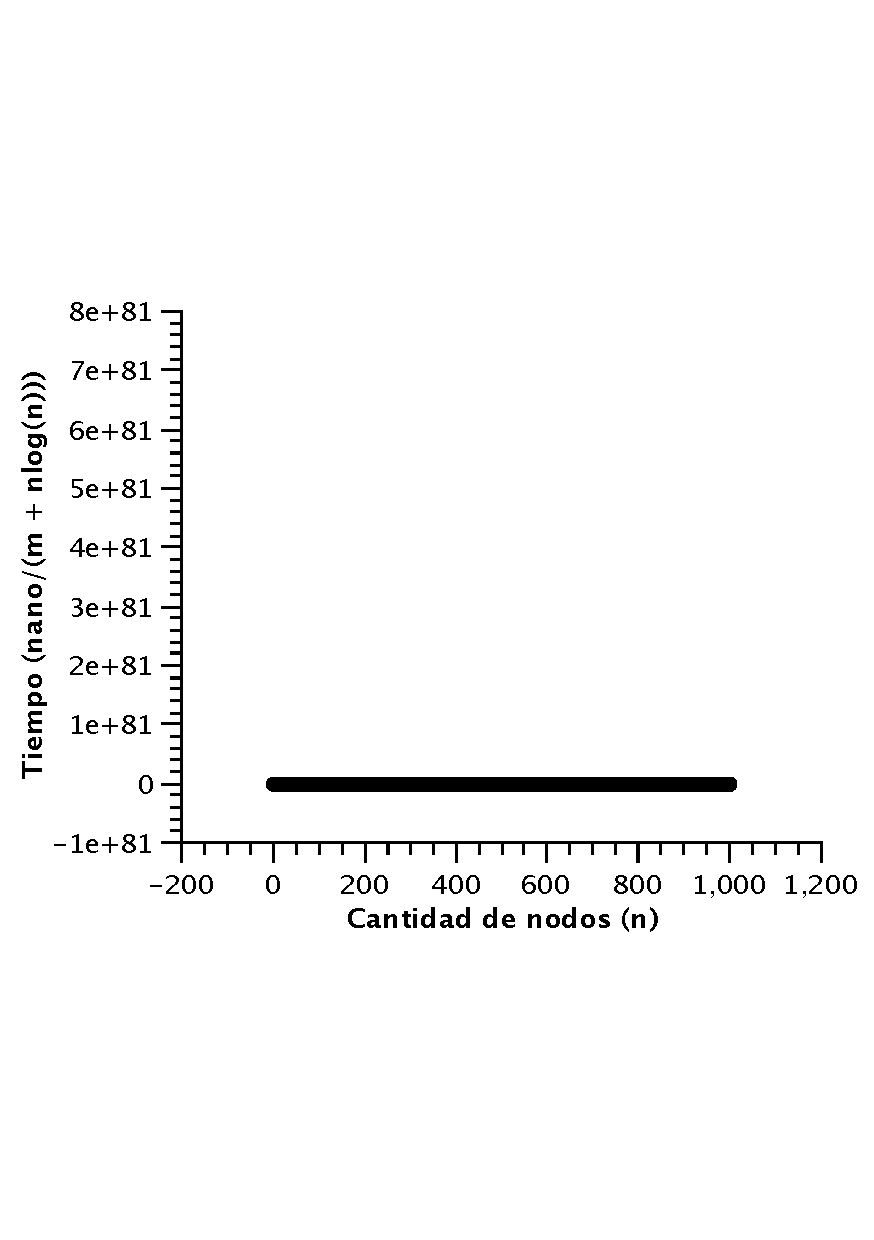
\includegraphics[width=\textwidth]{imagenes/vacio-listas-3.pdf}
                \caption{Dividiendo a los tiempos por $n^2$}
        \end{subfigure}

        \begin{subfigure}[b]{0.5\textwidth}
                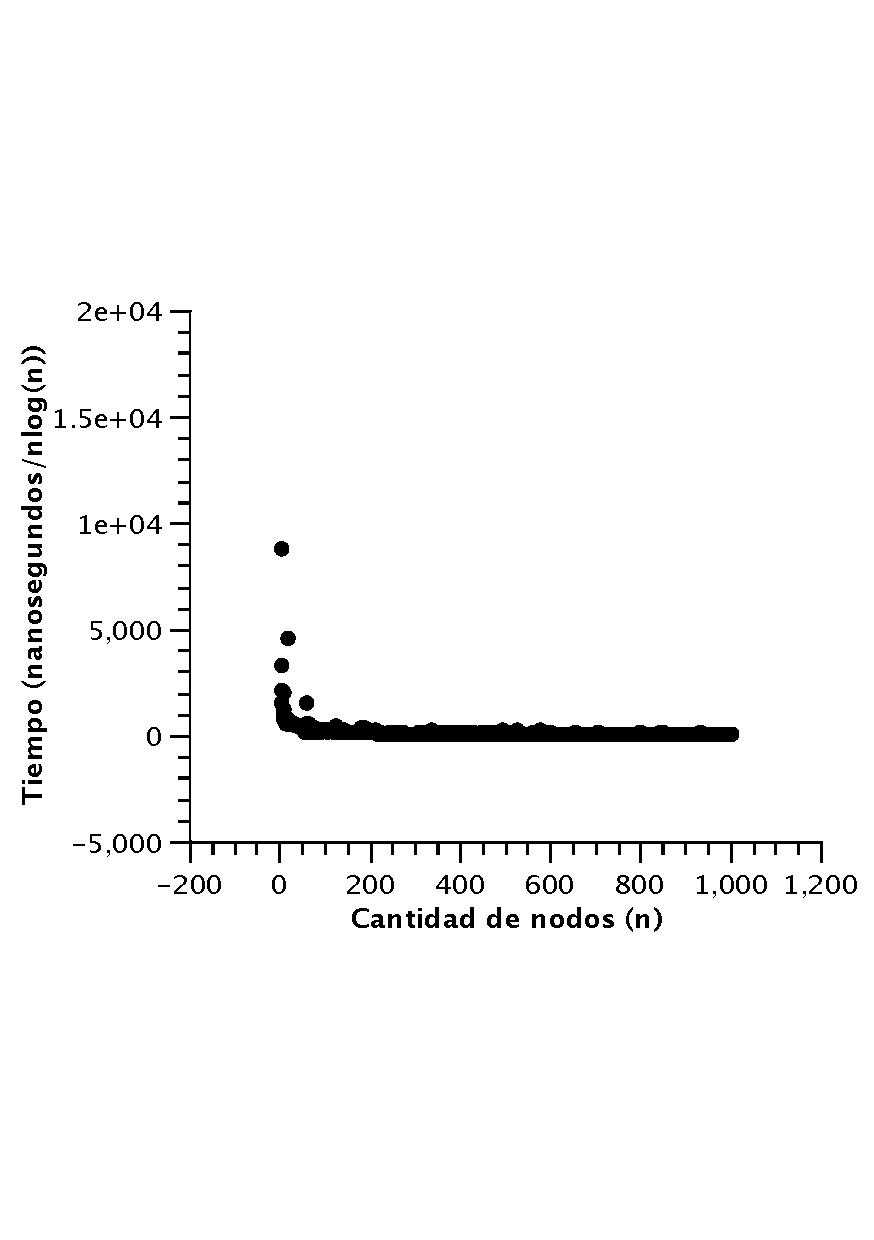
\includegraphics[width=\textwidth]{imagenes/vacio-listas-4.pdf}
                \caption{Dividiendo a los tiempos por $n + n*log(n)$}
        \end{subfigure}

\end{figure}

A continuación, adjuntamos una tabla con los últimos 20 valores obtenidos en las instancias, teniendo en cuenta que los casos fueron previamente ordenados según el tamaño ($n$):

\begin{table}[H]
\parbox{0.3\textwidth}{
    \begin{tabular}{ | l | l | l | l | l |}
    \hline
n   &Tiempo(milis) &Tiempo(mili/($n$)) &Tiempo(mili/($n^2$))) &Tiempo(mili/($n*log(n) + m$)))\\ \hline
980	&283,093	&288.87040816327	&0.2947657226155768	&96.57257621237783\\ \hline
981	&279,943	&285.36493374108	&0.2908918794506428	&95.38653274714977\\ \hline
982	&280,415	&285.5549898167	    &0.290789195332689	&95.43594581360509\\ \hline
983	&288,893	&293.88911495422	&0.2989716327102968	&98.20680338813817\\ \hline
984	&276,797	&281.29776422764	&0.2858717116134576	&93.98537417420873\\ \hline
985	&277,190	&281.41116751269	&0.2856966167641526	&94.00940786565884\\ \hline
986	&276,617	&280.54462474645	&0.2845280169842295	&93.70613178730468\\ \hline
987	&277,663	&281.3201621074	    &0.2850254935231977	&93.95135777670718\\ \hline
988	&281,872	&285.2955465587	    &0.2887606746545592	&95.26500875949687\\ \hline
989	&282,107	&285.24469160768	&0.2884172817064555	&95.23405608103857\\ \hline
990	&277,617	&280.42121212121	&0.283253749617386	&93.60993375526336\\ \hline
991	&278,533	&281.06256306761	&0.2836150989582326	&93.81029823710891\\ \hline
992	&278,372	&280.61693548387	&0.2828799752861603	&93.64786998548107\\ \hline
993	&278,950	&280.91641490433	&0.2828966917465562	&93.73412480887504\\ \hline
994	&279,345	&281.03118712274	&0.2827275524373606	&93.75874548093792\\ \hline
995	&279,336	&280.73969849246	&0.2821504507461933	&93.64785410306024\\ \hline
996	&278,955	&280.07530120482	&0.2812001016112644	&93.41263366232546\\ \hline
997	&283,107	&283.95887662989	&0.2848133165796286	&94.69414583300491\\ \hline
998	&283,434	&284.00200400802	&0.2845711463006173	&94.69477906957285\\ \hline
999	&283,640	&283.92392392392	&0.2842081320559799	&94.65501754783944\\ \hline
1,000	&284,062	&284.062	&0.284062	&94.68733333333333\\ \hline
    \end{tabular}
}
\end{table}

Como podemos ver, la experimentación se condice con el cálculo teórico de la complejidad y arroja que es de $\mathcal{O}(n*log(n) + m)$, sin embargo, como el grafo no tiene aristas, aqui la complejidad es de $\mathcal{O}(n*log(n))$ siendo así más eficiente que en la implementación sobre matriz de adyacencia.









\newpage
\section{Ejercicio 4 - Heurística de búsqueda local}
%\textit{Diseñar e implementar una heurística de búsqueda local para CIDM.}

\subsection{Ejercicio A}

\textit{Explicar detalladamente el algoritmo implementado. Plantear al menos dos vecindades distintas para la búsqueda y al menos dos soluciones iniciales.}

\medskip

\subsubsection{Algoritmo implementado}

Sea G=(V,E) un grafo simple, la heurística de búsqueda local propuesta genera una solución inicial valida, es decir un V' $\subseteq$ V que es dominante e independiente (CID), de dos formas:
\begin{enumerate}
	\item \textbf{Heurística constructiva golosa}: procedimiento descripto en el ejercicio anterior.
    \item \textbf{Procedimiento BFS modificado}: detallado a continuación.

\end{enumerate}

\subsubsection{Procedimiento BFS modificado:}

Partimos de incluir un vértice inicial $v$ a $V'$ y luego vamos a ir agregando vértices a $V'$ determinando si el vértice analizado debe incluirse en $V'$.
El BFS modificado funciona de la siguiente manera:
\medskip

\begin{codesnippet}
Los vértices están numerados de 0 a n-1.

Creamos un vector, llamado solucionInicial, de tamaño n para guardar el estado de los
vértices (si fue VISITADO o no)

Creamos un vector de tamaño n en donde para cada posición guardamos si
pertenece al CID (INCLUIDO o no)

Al vértice inicial v lo ponemos como VISITADO y INCLUIDO y lo incluimos en la cola.

Luego mientras no este vacía la cola:
    Sacamos el primer elemento de la cola (w) y lo ponemos INCLUIDO.
    Revisamos cada adyacente a w:
        Si algún adyacente esta INCLUIDO entonces hacemos w = NO INCLUIDO.
        Si el adyacente no fue VISITADO entonces lo ponemos como VISITADO y
        lo agregamos a la cola.

Repetimos el procedimiento para el resto de las componentes conexas, empezando por
el vértice de menor numeración de la componente analizada.
\end{codesnippet}

A continuación mostramos un ejemplo del recorrido BFS, en donde el vértice 0 ya fue visitado y se esta analizando sus adyacentes, en particular el vértice 1, el cual es provisoriamiente INCLUIDO:
\medskip

\tikz[every node/.style={draw,circle}] {
\node[fill=blue!40, text=white] (1) at (0, 0)  { 0 };
\node[fill=red!40, text=white] (2) at (2, 0)  { 1 };
\node (5) at (4, 0)  { 3 };
\node (6) at (6, 0)  { 4 };
\node (7) at (3,-1)  { 2 };
\draw (1) edge node[above,draw=none] {} (2);
\draw (5) edge node[above,draw=none] {} (6);
\draw (2) edge node[above,draw=none] {} (7);
}

Para luego ser desmarcado debido a la presencia de un adyacente INCLUIDO, siendo la solución generada la siguiente:
\medskip

\tikz[every node/.style={draw,circle}] {
\node[fill=blue!40, text=white] (1) at (0, 0)  { 0 };
\node (2) at (2, 0)  { 1 };
\node[fill=blue!40, text=white] (5) at (4, 0)  { 3 };
\node (6) at (6, 0)  { 4 };
\node[fill=blue!40, text=white] (7) at (3,-1)  { 2 };
\draw (1) edge node[above,draw=none] {} (2);
\draw (5) edge node[above,draw=none] {} (6);
\draw (2) edge node[above,draw=none] {} (7);
}



\subsubsection{Primer Criterio de Vecindad}

El primer criterio de vecindad implementado consiste en generar soluciones vecinas a partir de quitar k vértices que pertenecen al subconjunto CID de la solución inicial y agregar 1 vértice al subconjunto, donde k $\in \mathbb{N}$ y k $\geq$ 2. Logrando de esta manera una reducción en el cardinal del subconjunto CID de, al menos, un vértice.

Para llevar adelante exitosamente este intercambio, debemos buscar aquellos vértices no incluidos en CID en la solución inicial, que tengan, al menos, dos vértices adyacentes incluidos en CID, para poder incluir ese vértice en la solución vecina y quitar sus adyacentes.

\begin{itemize}
	\item Ejemplo de un cambio 4 por 1:

    \tikz[every node/.style={draw,circle}] {
		\node[fill=blue!40, text=white] (1) at (0, 0)  { 0 };
		\node (2) at (1, -1)  { 1 };
		\node[fill=blue!40, text=white] (5) at (2, -2)  { 3 };
		\node[fill=blue!40, text=white] (7) at (2, 0)  { 2 };
		\node[fill=blue!40, text=white] (8) at (0, -2)  { 4 };
		\node (9) at (5, 0)  { 0 };
		\node[fill=blue!40, text=white] (10) at (6, -1)  { 1 };
		\node (11) at (7, -2)  { 3 };
		\node (12) at (7, 0)  { 2 };
		\node (13) at (5, -2)  { 4 };
		\draw (1) edge node[above,draw=none] {} (2);
		\draw (5) edge node[above,draw=none] {} (2);
		\draw (2) edge node[above,draw=none] {} (7);
		\draw (2) edge node[above,draw=none] {} (8);
		\draw (9) edge node[above,draw=none] {} (10);
		\draw (11) edge node[above,draw=none] {} (10);
		\draw (10) edge node[above,draw=none] {} (12);
		\draw (10) edge node[above,draw=none] {} (13);
}

\end{itemize}

Sin embargo, para lograr una solución valida, los vértices quitados no pueden tener otros vértices adyacentes no incluidos en el subconjunto que, a su vez, no sean adyacentes al vértice agregado  y no sean dominados por otro vértice.

\begin{itemize}
	\item Ejemplo de solucion invalida:

    \tikz[every node/.style={draw,circle}] {
		\node[fill=blue!40, text=white] (1) at (0, 0)  { 0 };
		\node (2) at (1, -1)  { 1 };
		\node[fill=blue!40, text=white] (5) at (2, -2)  { 3 };
		\node[fill=blue!40, text=white] (7) at (2, 0)  { 2 };
		\node[fill=blue!40, text=white] (8) at (0, -2)  { 4 };
		\node (14) at (3.5, 0)  { 5 };
		\node (9) at (5, 0)  { 0 };
		\node[fill=blue!40, text=white] (10) at (6, -1)  { 1 };
		\node (11) at (7, -2)  { 3 };
		\node (12) at (7, 0)  { 2 };
		\node (13) at (5, -2)  { 4 };
		\node (15) at (8.5, 0)  { 5 };
		\draw (1) edge node[above,draw=none] {} (2);
		\draw (5) edge node[above,draw=none] {} (2);
		\draw (2) edge node[above,draw=none] {} (7);
		\draw (2) edge node[above,draw=none] {} (8);
		\draw (7) edge node[above,draw=none] {} (14);
		\draw (9) edge node[above,draw=none] {} (10);
		\draw (11) edge node[above,draw=none] {} (10);
		\draw (10) edge node[above,draw=none] {} (12);
		\draw (10) edge node[above,draw=none] {} (13);
		\draw (12) edge node[above,draw=none] {} (15);
}

\end{itemize}

El procedimiento de búsqueda de los posibles soluciones vecinas funciona de la siguiente manera:
\medskip

\begin{codesnippet}
Para todo vertice, u, en el Grafo:
  Creamos un vector de tamaño n, llamado solucionAuxiliar, al cual le copiamos
  el contenido de la solucionInicial.
  Si solucionInicial[u] = NO INCLUIDO y |adyacentes a u| > 1 entonces:
     solucionAuxiliar[u] = INCLUIDO
     cantAdyacentesIncluidos = 0
     Para todo adyacente, v, de u:
         Si solucionInicial[v] = INCLUIDO entonces:
             cantAdyacentesIncluidos ++
             solucionAuxiliar[v] = NO INCLUIDO

  Si cantAdyacentesIncluidos > 1 entonces:
     Si esSolucion?(solucionAuxiliar) entonces:
       Buscar Nuevos Vecinos a partir de la solucionAuxiliar
       Interrumpir el ciclo
\end{codesnippet}

En el procedimiento descripto anteriormente falta detallar el comportamiento de la funciona auxiliar \textit{esSolucion?}, la cual sera descripta en el apartado siguiente, ya que es utilizado por ambos criterios.

\subsubsection{Segundo Criterio de Vecindad}
El segundo criterio de vecindad implementado consiste en generar soluciones vecinas a partir de quitar k vértices que pertenecen al subconjunto CID de la solución inicial y agregar, hasta, k-1 vértices al subconjunto, donde k $\in \mathbb{N}$ y k $\geq$ 2. Logrando de esta manera, una reducción en el cardinal del subconjunto CID de, al menos, un vértice.
El caso donde k = 2 no difiere del criterio aplicado en la primer vecindad, ya que k - 1 = 1. Sin embargo a partir de k $\geq$ 3 se observa un comportamiento distinto, ya que podemos agregar k-2 vértices para arreglar la solución, ademas del candidato original.

En este caso, para los casos no contemplados en el criterio anterior, debemos buscar vértices no incluidos en CID en la solución inicial, que tengan, al menos k vértices adyacentes incluidos en CID, donde k $\geq$ 3, y que a su vez tengan hasta k-2 vértices que son adyacentes a los adyacentes del vertice buscado que no estan incluidos y no son dominados por otro vértice.

\begin{itemize}
	\item Ejemplo de un caso 4-2, el cual fallaba en el criterio anterior:

    \tikz[every node/.style={draw,circle}] {
		\node[fill=blue!40, text=white] (1) at (0, 0)  { 0 };
		\node (2) at (1, -1)  { 1 };
		\node[fill=blue!40, text=white] (5) at (2, -2)  { 3 };
		\node[fill=blue!40, text=white] (7) at (2, 0)  { 2 };
		\node[fill=blue!40, text=white] (8) at (0, -2)  { 4 };
		\node (14) at (3.5, 0)  { 5 };
		\node (9) at (5, 0)  { 0 };
		\node[fill=blue!40, text=white] (10) at (6, -1)  { 1 };
		\node (11) at (7, -2)  { 3 };
		\node (12) at (7, 0)  { 2 };
		\node (13) at (5, -2)  { 4 };
		\node[fill=blue!40, text=white] (15) at (8.5, 0)  { 5 };
		\draw (1) edge node[above,draw=none] {} (2);
		\draw (5) edge node[above,draw=none] {} (2);
		\draw (2) edge node[above,draw=none] {} (7);
		\draw (2) edge node[above,draw=none] {} (8);
		\draw (7) edge node[above,draw=none] {} (14);
		\draw (9) edge node[above,draw=none] {} (10);
		\draw (11) edge node[above,draw=none] {} (10);
		\draw (10) edge node[above,draw=none] {} (12);
		\draw (10) edge node[above,draw=none] {} (13);
		\draw (12) edge node[above,draw=none] {} (15);
}

\end{itemize}

\begin{itemize}
	\item Caso donde falla el segundo criterio:

    \tikz[every node/.style={draw,circle}] {
		\node (1)[fill=blue!40, text=white] at (0, 0)  { 0 };
		\node (2) at (1, -1)  { 1 };
		\node (3)[fill=blue!40, text=white] at (2, 0)  { 2 };
		\node (4)[fill=blue!40, text=white] at (2, -2)  { 3 };
		\node (5) at (3.5, 0)  { 4 };
		\node (6) at (3.5, -2)  { 5 };
		\node (7) at (5, 0)  { 0 };
		\node (8)[fill=blue!40, text=white] at (6, -1)  { 1 };
		\node (9) at (7, 0)  { 2 };
		\node (10) at (7, -2)  { 3 };
		\node (11)[fill=blue!40, text=white] at (8.5, 0)  { 4 };
		\node (12) at (8.5, -2)  { 5 };
		\draw (1) edge node[above,draw=none] {} (2);
		\draw (2) edge node[above,draw=none] {} (3);
		\draw (2) edge node[above,draw=none] {} (4);
		\draw (3) edge node[above,draw=none] {} (5);
		\draw (4) edge node[above,draw=none] {} (6);
		\draw (7) edge node[above,draw=none] {} (8);
		\draw (8) edge node[above,draw=none] {} (9);
		\draw (8) edge node[above,draw=none] {} (10);
		\draw (9) edge node[above,draw=none] {} (11);
		\draw (10) edge node[above,draw=none] {} (12);
}

\end{itemize}

El procedimiento de búsqueda de los posibles soluciones vecinas funciona de la siguiente manera:
\medskip

\begin{codesnippet}
Para todo vértice, u, en el Grafo:
  Creamos un vector de tamaño n, llamado solucionAuxiliar, al cual le copiamos
  el contenido de la solucionInicial.
  Si solucionInicial[u] = NO INCLUIDO y |adyacentes a u| > 1 entonces:
     solucionAuxiliar[u] = INCLUIDO
     cantAdyacentesIncluidos = 0
     Para todo adyacente, v, de u:
         Si solucionInicial[v] = INCLUIDO entonces:
             cantAdyacentesIncluidos ++
             solucionAuxiliar[v] = NO INCLUIDO

  Si cantAdyacentesIncluidos > 1 entonces:
     cantCambiosPosibles = cantAdyacentesIncluidos - 2
     arreglarSolucion(solucionAuxiliar, cantCambiosPosibles)
     Si esSolucion?(solucionAuxiliar) entonces:
       Buscar Nuevos Vecinos a partir de la solucionAuxiliar
       Interrumpir el ciclo
\end{codesnippet}

FFalta detallar los procedimientos \textit{arreglarSolucion} y \textit{esSolucion?}, los cuales se pueden realizar en una sola función que llamaremos \textit{esSolucion?} cuyo comportamiento es el siguiente:
\begin{itemize}
	\item La función recibe como parámetros un vector con la solución a analizar y un entero con la cantidad de cambios posibles a realizar
	\item Miramos cada vértice del grafo, los cuales o están INCLUIDOS o NO INCLUIDOS en el subconjunto CID.
    \item Si el vértice esta INCLUIDO, sus adyacentes NO pueden estar INCLUIDOS. En caso de encontrar algun adyacente INCLUIDO, sabemos que el subconjunto analizado no es solución valida.
    \item Si el vértice NO esta INCLUIDO, entonces, al menos, 1 vértice adyacente tiene que estar INCLUIDO. En caso de no encontrar algún vértice adyacente INCLUIDO, tenemos dos casos:
    \begin{enumerate}
    	\item La variable entera que representa la cantidad de cambios posibles es 0. En este caso sabemos que el subconjunto analizado no es solución valida.
        \item La variable entera que representa la cantidad de cambios posibles es mayor a 0. En este caso el vértice pasa a estar INCLUIDO en el subconjunto, manteniéndose la validez de la solución, ya que el vértice NO tiene adyacentes INCLUIDOS. También reducimos la cantidad de cambios posibles en una unidad.
    \end{enumerate}

    \item En pseudocódigo:

\end{itemize}

\begin{codesnippet}
Como entrada tenemos el vector solucionAuxiliar con la solución a analizar y el entero
cantCambiosPosibles, que tiene la cantidad de vértices que podemos incluir.

Creamos una variable booleana, esSolucion inicializada en true.

Luego, para todo vértice, u, en el Grafo:
  Si solucionAuxiliar[u] = INCLUIDO y |adyacentes a u| > 0 entonces:
     Para todo adyacente, v, de u:
         Si solucionInicial[v] = INCLUIDO entonces:
             esSolucion = false
             Interrumpir el ciclo

  Sino Si |adyacentes a u| > 0, entonces:
       adyacenteIncluido = false
       Para todo adyacente, v, a u:
          Si solucionInicial[v] = INCLUIDO entonces:
             adyacenteIncluido = true
       Si not(adyacenteIncluido) y cantCambiosPosibles = 0 entonces:
         esSolucion = false
         Interrumpir el ciclo
       Sino Si not(adyacenteIncluido) entonces:
         solucionAuxiliar[u] = INCLUIDO
         cantCambiosPosibles --

  Sino entonces:
       esSolucion = (solucionAuxiliar[u] = INCLUIDO)
\end{codesnippet}

Es necesario aclarar que para el primer criterio de vecindad, la cantidad de cambios posibles es 0.

\subsection{Ejercicio B}

\textit{Calcular el orden de complejidad temporal de peor caso de una iteración del algoritmo.}
\medskip

La estructura de datos que utilizamos para representar los grafos son vectores con listas, donde cada posición del vector representa un vértice y las listas contienen los adyacentes a ese vértice.

A partir de los procedimientos expuestos en el punto anterior, pasamos a analizar la complejidad de la heurística propuesta, para solo una iteración:

\begin{enumerate}
  \item \textbf{Solución Inicial}
    \begin{itemize}
    	\item \underline{Heurística Golosa}: $\mathcal{O}(n*log(n) + m)$. Justificada anteriormente.
        \item \underline{BFS modificado}: Las cambios implementados en el BFS no alteran su complejidad original, siendo la misma $\mathcal{O}(n + m)$. \footnote{Referencia \url{https://en.wikipedia.org/wiki/Breadth-first_search}}
    \end{itemize}
  \item \textbf{Primer Criterio de Vecindad}

  Tenemos un ciclo que se repite $n$ veces, el cual tiene varias operaciones que se realizan internamente:
  \begin{itemize}
    \item Creación de un vector tamaño $n$ y copia de contenido: $\Theta{(n)}$
    \item Comparaciones y Asignaciones: $\mathcal{O}(1)$
    \item Ciclo de los adyacentes, cuya complejidad, sumada a la del ciclo principal, es $\mathcal{O}(n + m)$.
    \item Complejidad de la función esSolucion?: $\mathcal{O}(n + m)$. Detallada en el punto 4.
  \end{itemize}
  Por lo tanto la complejidad total de este procedimiento es: $\mathcal{O}(n*(n + n + m) + n + m)$, lo cual es: $\mathcal{O}(n*(n + m))$

  \item \textbf{Segundo Criterio de Vecindad}

    Misma situación que el punto anterior, tenemos un ciclo que se repite $n$ veces, el cual tiene varias operaciones que se realizan internamente:
  \begin{itemize}
    \item Creación de un vector tamaño $n$ y copia de contenido: $\Theta{(n)}$
    \item Comparaciones y Asignaciones: $\mathcal{O}(1)$
    \item Ciclo de los adyacentes, cuya complejidad, sumada a la del ciclo principal, es $\mathcal{O}(n + m)$.
    \item Complejidad de la función esSolucion?: $\mathcal{O}(n + m)$. Detallada en el punto 4.
  \end{itemize}
  Por lo tanto la complejidad total de este procedimiento es: $\mathcal{O}(n*(n + n + m) + n + m)$, lo cual es: $\mathcal{O}(n*(n + m))$

  \item \textbf{Procedimiento esSolucion?}

    Tenemos un ciclo que se repite $n$ veces, el cual tiene varias operaciones que se realizan internamente:
  \begin{itemize}
    \item Comparaciones y Asignaciones: $\mathcal{O}(1)$
    \item Ciclo de los adyacentes, cuya complejidad, sumada a la del ciclo principal, es $\mathcal{O}(n + m)$.
  \end{itemize}
  Por lo tanto la complejidad total de este procedimiento es: $\mathcal{O}(n + m)$.

\end{enumerate}

Podemos concluir que la complejidad temporal de la heurística es independiente del procedimiento utilizado para armar la solución inicial, y que utilizando el primer o segundo criterio de vecindad la complejidad es la misma: $\mathcal{O}(n*(n + m))$.\\

\medskip

\textbf{Cota superior para la cantidad de iteraciones:}
\medskip

Sabemos que cada iteración de las vecindades reduce, como mínimo, en 1 el cardinal del subconjunto CID. Por lo tanto, si partimos de una solución inicial en donde el cardinal del subconjunto es asintonticamente igual a la cantidad de vértices del Grafo, es posible que iteraremos hasta n-1 veces, hasta alcanzar una solución de 1 vértice. Es evidente que este es un caso extremo, de difícil realización, sin embargo brinda una cota superior a la cantidad de iteraciones.

\subsection{Ejercicio C}

\textit{Realizar una experimentación que permita observar la perfomance del algoritmo comparando los tiempos de ejecución y la calidad de las soluciones obtenidas.}

\medskip

La función que utilizamos para llevar a cabo las mediciones fue \texttt{std::clock}\footnote{Referencia \url{http://en.cppreference.com/w/cpp/chrono/c/clock}}. La unidad temporal que utilizamos para este ejercicio fue nanosegundos.
La complejidad teórica calculada es de $\mathcal{O}(n*(n + m))$ para cualquier combinación de solución inicial y criterio de vecindad.

Para generar las instancias aleatorias utilizamos la función \texttt{std::rand}\footnote{Referencia \url{http://en.cppreference.com/w/cpp/numeric/random/rand}} con determinados intervalos de valores para la variables, para obtener instancias coherentes. El detalle de intervalos es el siguiente:

\begin{enumerate}
	\item Cantidad de nodos $n$: 2 $\leq$ $n$ $\leq$ 50.
    \item Cantidad de aristas $m$: 0 $\leq$ $m$ $\leq$ $\frac{n*(n-1)}{2}$.
    \item Se generan $m$ ejes, asegurándose la validez de los mismos, es decir que no haya ejes repetidos ni loops.
\end{enumerate}

Se generaron 500 instancias construidas de esta forma, en donde se midió no solo el tiempo de ejecución, sino también el tamaño del subconjunto generado, para los 4 tipos contemplados en la heurística:

\begin{itemize}
	\item Tipo B1: Utilizamos el BFS modificado para la solución original, y el primer criterio de vecindad.
    \item Tipo G1: Utilizamos la heurística golosa para la solución original, y el primer criterio de vecindad.
    \item Tipo B2: Utilizamos el BFS modificado para la solución original, y el segundo criterio de vecindad.
    \item Tipo G2: Utilizamos la heurística golosa para la solución original, y el segundo criterio de vecindad.
\end{itemize}

La medición de tiempos de los distintos tipos, arroja los siguientes gráficos para cada tipo:

\begin{enumerate}
\item \textbf{Tipo B1: BFS-Primer Criterio de Vecindad}

\begin{figure}[H]
        \centering
        \begin{subfigure}[b]{0.5\textwidth}
                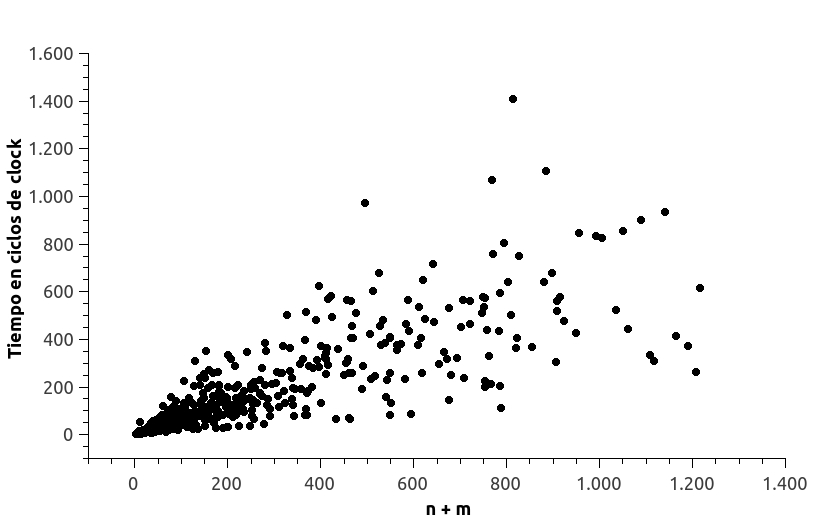
\includegraphics[width=\textwidth]{imagenes/ejer4-grafB1-1.jpg}
                \caption{Tiempos sin procesar}
        \end{subfigure}%
        ~ %add desired spacing between images, e. g. ~, \quad, \qquad, \hfill etc.
          %(or a blank line to force the subfigure onto a new line)
        \begin{subfigure}[b]{0.5\textwidth}
                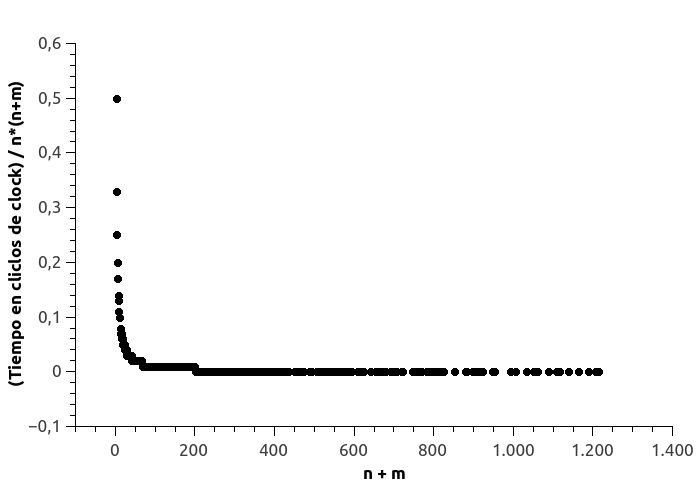
\includegraphics[width=\textwidth]{imagenes/ejer4-grafB1-2.jpg}
                \caption{figura (a) / n*(n+m)}
        \end{subfigure}

\end{figure}

\item \textbf{Tipo G1: Goloso-Primer Criterio de Vecindad}

\begin{figure}[H]
        \centering
        \begin{subfigure}[b]{0.5\textwidth}
                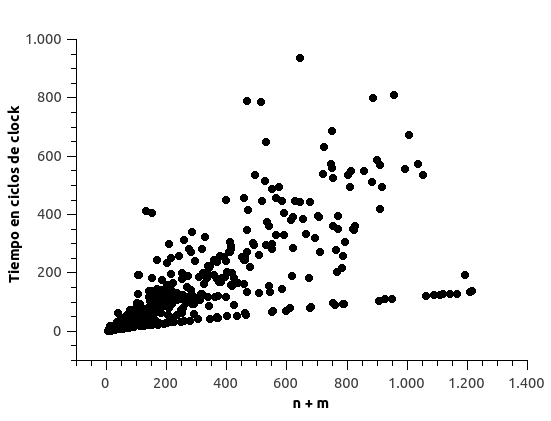
\includegraphics[width=\textwidth]{imagenes/ejer4-grafG1-1.jpg}
                \caption{Tiempos sin procesar}
        \end{subfigure}%
        ~ %add desired spacing between images, e. g. ~, \quad, \qquad, \hfill etc.
          %(or a blank line to force the subfigure onto a new line)
        \begin{subfigure}[b]{0.5\textwidth}
                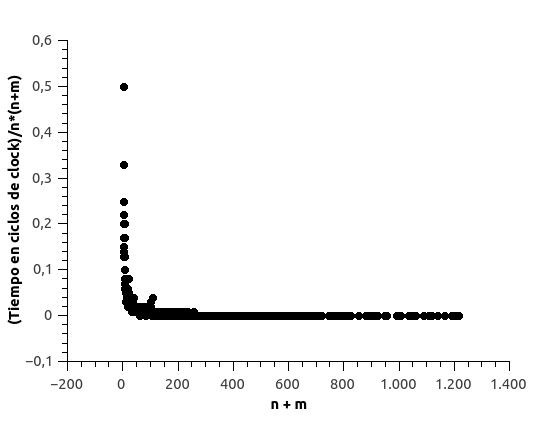
\includegraphics[width=\textwidth]{imagenes/ejer4-grafG1-2.jpg}
                \caption{figura (a) / n*(n+m)}
        \end{subfigure}

\end{figure}


\item \textbf{Tipo B2: BFS-Segundo Criterio de Vecindad}

\begin{figure}[H]
        \centering
        \begin{subfigure}[b]{0.5\textwidth}
                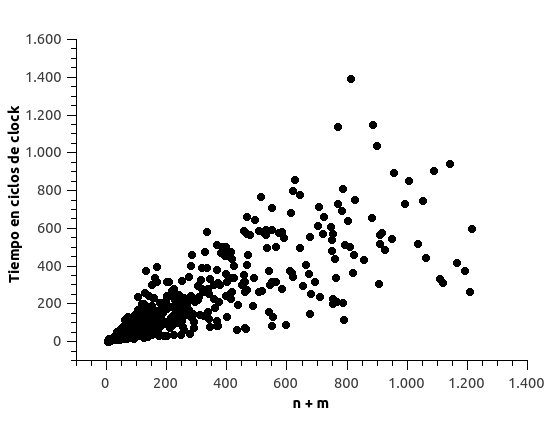
\includegraphics[width=\textwidth]{imagenes/ejer4-grafB2-1.jpg}
                \caption{Tiempos sin procesar}
        \end{subfigure}%
        ~ %add desired spacing between images, e. g. ~, \quad, \qquad, \hfill etc.
          %(or a blank line to force the subfigure onto a new line)
        \begin{subfigure}[b]{0.5\textwidth}
                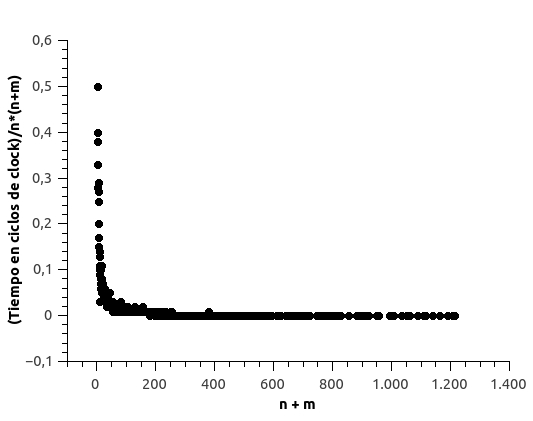
\includegraphics[width=\textwidth]{imagenes/ejer4-grafB2-2.jpg}
                \caption{figura (a) / n*(n+m)}
        \end{subfigure}

\end{figure}



\item \textbf{Tipo G2: Goloso-Segundo Criterio de Vecindad}

\begin{figure}[H]
        \centering
        \begin{subfigure}[b]{0.5\textwidth}
                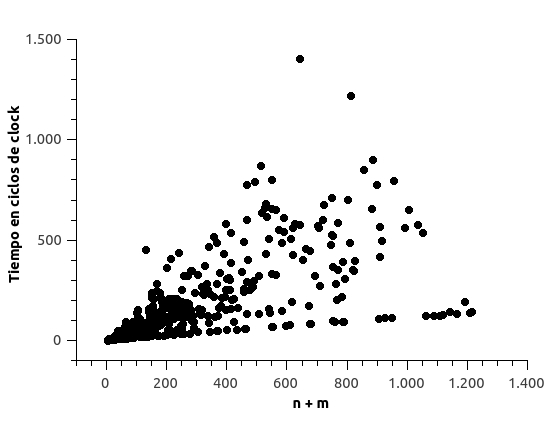
\includegraphics[width=\textwidth]{imagenes/ejer4-grafG2-1.jpg}
                \caption{Tiempos sin procesar}
        \end{subfigure}%
        ~ %add desired spacing between images, e. g. ~, \quad, \qquad, \hfill etc.
          %(or a blank line to force the subfigure onto a new line)
        \begin{subfigure}[b]{0.5\textwidth}
                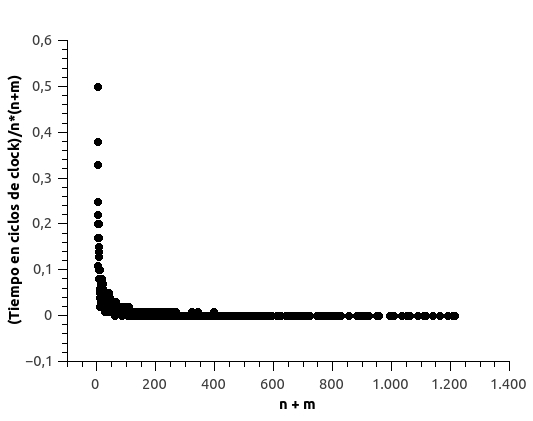
\includegraphics[width=\textwidth]{imagenes/ejer4-grafG2-2.jpg}
                \caption{figura (a) / n*(n+m)}
        \end{subfigure}

\end{figure}


\end{enumerate}

Como podemos ver de los 4 gráficos, al dividir los tiempos por $n*(n+m)$, tienden a un número constante mayor a cero. Entonces nuestro algoritmo tendría complejidad $\mathcal{O}(c*n*(n+m))$, donde $c$ es la constante a la cual converge el gráfico. Por lo tanto concluimos que la complejidad temporal experimental coincide con nuestra predicción de complejidad.


Por el lado de la calidad de las soluciones obtenidas con cada combinación, debemos comparar por un lado el uso del BFS modificado o de la heurística golosa como solución inicial y por el otro el uso del primer criterio de vecindad o el del segundo criterio de vecindad como método de mejora de la solución inicial:
\begin{itemize}
\item \textbf{BFS modificado vs Heurística golosa como solución inicial}. Para realizar la comparación, tomamos el tamaño de la solución final para cada instancia, usando primero el BFS modificado como solución inicial y luego la heurística golosa, para después restar al tamaño de la solución final del tipo B1/B2, el tamaño de la solución final del tipo G1/G2. :

\begin{figure}[H]
        \centering
        \begin{subfigure}[b]{0.5\textwidth}
                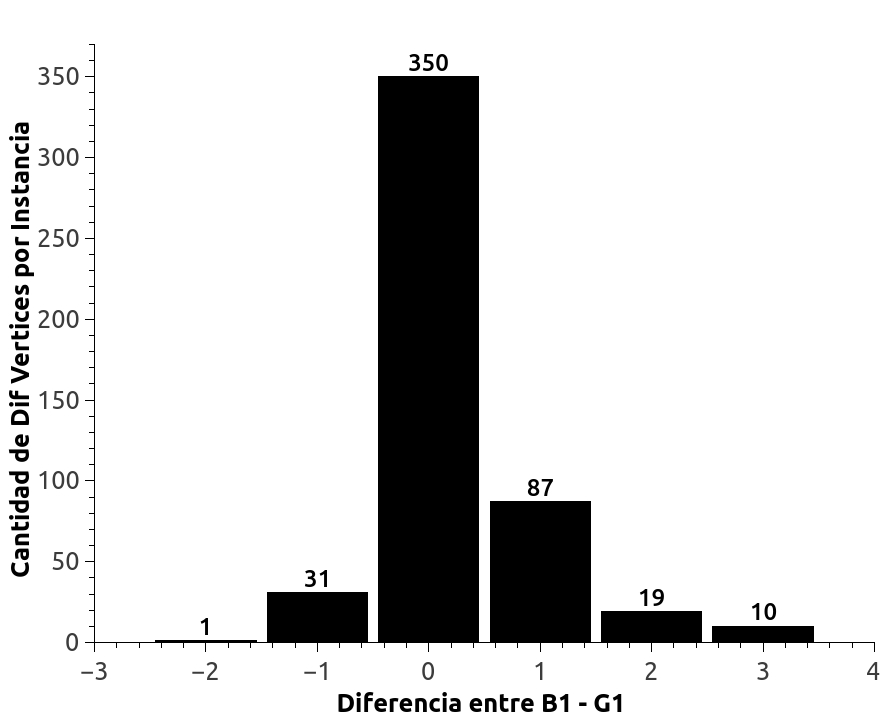
\includegraphics[width=\textwidth]{imagenes/ejer4-B1vsG1.jpg}
                \caption{Usando el Primer Criterio de Vecindad}
        \end{subfigure}%
        ~ %add desired spacing between images, e. g. ~, \quad, \qquad, \hfill etc.
          %(or a blank line to force the subfigure onto a new line)
        \begin{subfigure}[b]{0.5\textwidth}
                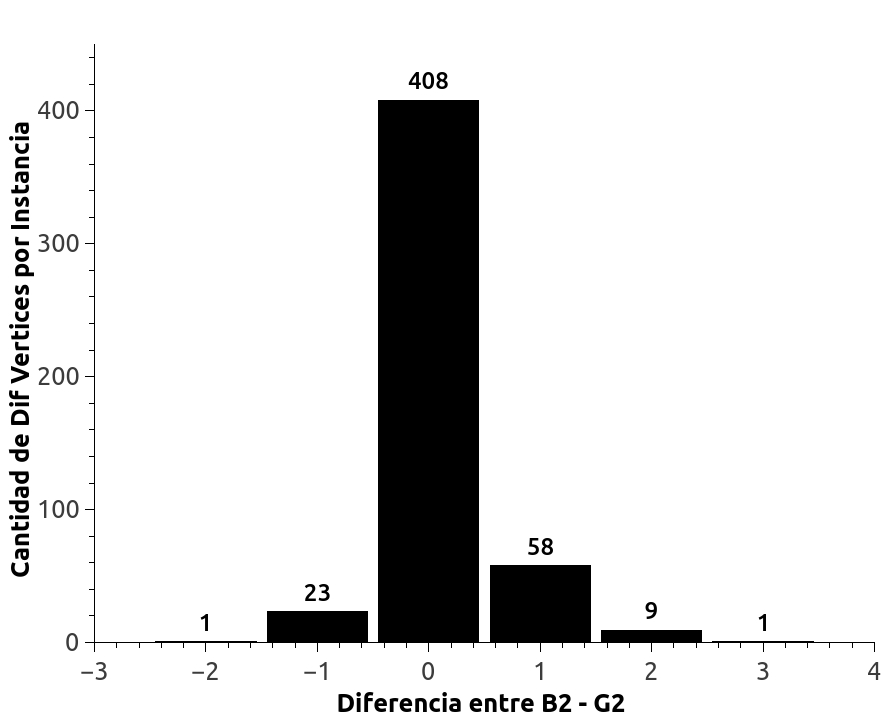
\includegraphics[width=\textwidth]{imagenes/ejer4-B2vsG2.jpg}
                \caption{Usando el Segundo Criterio de Vecindad}
        \end{subfigure}

\end{figure}

\end{itemize}

En ambos casos, se aprecia una paridad entre ambos soluciones, sin embargo hay una leve tendencia hacia la heurística golosa como mejor procedimiento para construir la solución inicial.

\begin{itemize}
	\item \textbf{Criterio de Vencindad}. El análisis comparado es el siguiente (utilizando la misma metodología que en el caso de BFS vs Golosa):

    \begin{figure}[H]
        \centering
        \begin{subfigure}[b]{0.5\textwidth}
                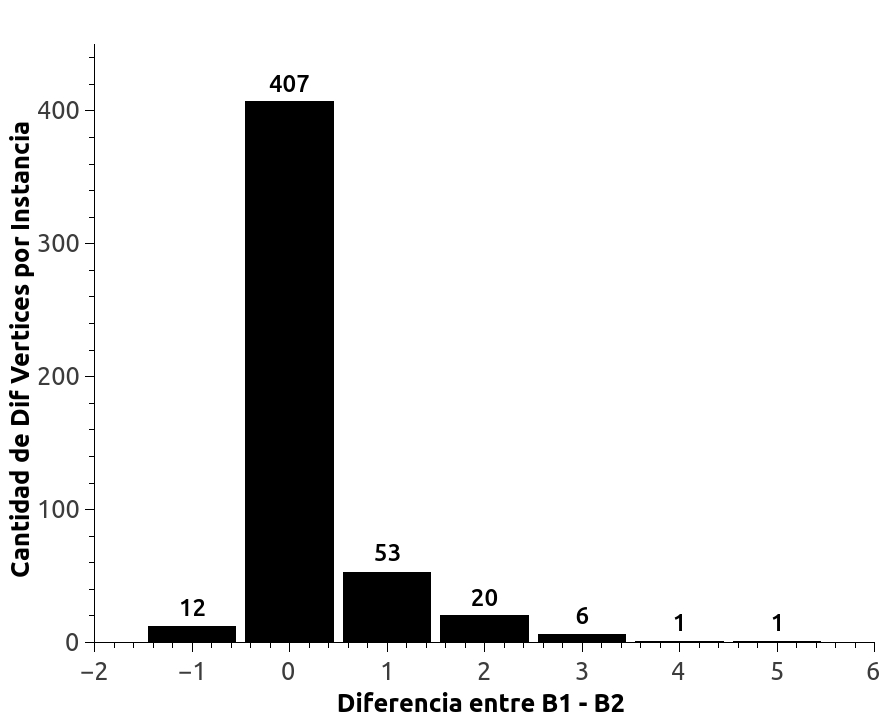
\includegraphics[width=\textwidth]{imagenes/ejer4-B1vsB2.jpg}
                \caption{Usando BFS como solucion incial}
        \end{subfigure}%
        ~ %add desired spacing between images, e. g. ~, \quad, \qquad, \hfill etc.
          %(or a blank line to force the subfigure onto a new line)
        \begin{subfigure}[b]{0.5\textwidth}
                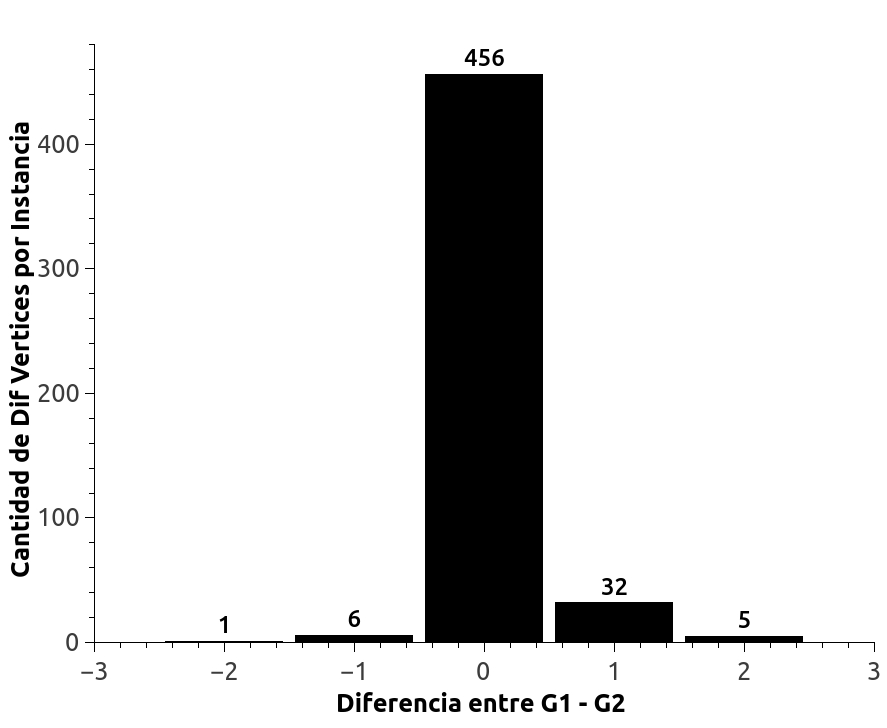
\includegraphics[width=\textwidth]{imagenes/ejer4-G1vsG2.jpg}
                \caption{Usando Goloso como solucion incial}
        \end{subfigure}

\end{figure}


\end{itemize}



Estos resultados nos inclinan a pensar que el segundo criterio de vecindad es el mejor criterio, lo cual es coherente con el hecho que el segundo criterio de vecindad es capaz de arreglar soluciones que el primer criterio de vecindad da como invalidas. Es decir, podríamos argumentar que como el primer criterio de vecindad es un caso particular del segundo criterio de vecindad (cuando no incluimos ningún vértice al subconjunto, mas allá del candidato) debería ser siempre mejor al primero. Sin embargo, la experimentación muestra casos donde el primer criterio es mejor, y eso se da en instancias donde arreglar una solución invalida nos inhibe de seguir explorando la solución original en búsqueda de un mejor caso. Por ejemplo:

\begin{itemize}

	\item Grafo de n = 9 y m = 13

\tikz[every node/.style={draw,circle}] {
	\node (1) at (0, 0)  { 1 };
	\node (2) at (4.5, 0)  { 2 };
	\node (3) at (2, -2)  { 3 };
	\node (4) at (2, 2)  { 4 };
	\node (5) at (7.5, -1.5)  { 5 };
	\node (6) at (1, -1)  { 6 };
	\node (7) at (3, 0)  { 7 };
	\node (8) at (2.5, -1)  { 8 };
	\node (9) at (4, -1)  { 9 };
	\draw (1) edge node[above,draw=none] {} (6);
	\draw (3) edge node[above,draw=none] {} (5);
	\draw (4) edge node[above,draw=none] {} (6);
	\draw (6) edge node[above,draw=none] {} (7);
	\draw (6) edge node[above,draw=none] {} (3);
	\draw (5) edge node[above,draw=none] {} (4);
	\draw (7) edge node[above,draw=none] {} (4);
	\draw (7) edge node[above,draw=none] {} (8);
	\draw (9) edge node[above,draw=none] {} (8);
	\draw (9) edge node[above,draw=none] {} (5);
	\draw (9) edge node[above,draw=none] {} (2);
	\draw (7) edge node[above,draw=none] {} (2);
	\draw (8) edge node[above,draw=none] {} (3);
}



\item \textbf{Solución Golosa}: como el mayor grado, 3, es compartido por varios vertices, empezamos por el menor numero de etiqueta, que es el 5, y asi sucesivamente.

\tikz[every node/.style={draw,circle}] {
	\node (1) at (0, 0)  { 1 };
	\node (2)[fill=blue!40, text=white] at (4.5, 0)  { 2 };
	\node (3) at (2, -2)  { 3 };
	\node (4) at (2, 2)  { 4 };
	\node (5)[fill=blue!40, text=white] at (7.5, -1.5)  { 5 };
	\node (6)[fill=blue!40, text=white] at (1, -1)  { 6 };
	\node (7) at (3, 0)  { 7 };
	\node (8)[fill=blue!40, text=white] at (2.5, -1)  { 8 };
	\node (9) at (4, -1)  { 9 };
	\draw (1) edge node[above,draw=none] {} (6);
	\draw (3) edge node[above,draw=none] {} (5);
	\draw (4) edge node[above,draw=none] {} (6);
	\draw (6) edge node[above,draw=none] {} (7);
	\draw (6) edge node[above,draw=none] {} (3);
	\draw (5) edge node[above,draw=none] {} (4);
	\draw (7) edge node[above,draw=none] {} (4);
	\draw (7) edge node[above,draw=none] {} (8);
	\draw (9) edge node[above,draw=none] {} (8);
	\draw (9) edge node[above,draw=none] {} (5);
	\draw (9) edge node[above,draw=none] {} (2);
	\draw (7) edge node[above,draw=none] {} (2);
	\draw (8) edge node[above,draw=none] {} (3);
}


\item \textbf{Solución aplicando el segundo criterio de vecindad a la solución golosa}: tenemos 4 candidatos que cumplen con el hecho de tener 2 o mas adyacentes incluidos: 3, 4, 7, 9.
\begin{enumerate}
	\item Vértice 3: incluimos el 3, quitamos el 5, 6 y 8, por lo tanto podemos incluir un vértice mas, que sera el 1. Sin embargo el 4 no es dominado por nadie, por lo cual no es una solución valida.
		\item Vértice 4: incluimos el 4, y quitamos el 5 y el 6. No podemos incluir ningún vértice mas, por lo tanto el 1 no es dominado por nadie, no es una solución valida.
		\item Vértice 7: incluimos el 7 y quitamos el 2, 6 y 8. Incluimos el 1, y nos queda una solución valida.
		\item Vértice 9: no es contemplado, ya que obtuvimos una solución mejor con el vértice 7. Solución que ya no es posible mejorar.
\end{enumerate}
\tikz[every node/.style={draw,circle}] {
	\node (1)[fill=blue!40, text=white] at (0, 0)  { 1 };
	\node (2) at (4.5, 0)  { 2 };
	\node (3) at (2, -2)  { 3 };
	\node (4) at (2, 2)  { 4 };
	\node (5)[fill=blue!40, text=white] at (7.5, -1.5)  { 5 };
	\node (6) at (1, -1)  { 6 };
	\node (7)[fill=blue!40, text=white] at (3, 0)  { 7 };
	\node (8) at (2.5, -1)  { 8 };
	\node (9) at (4, -1)  { 9 };
	\draw (1) edge node[above,draw=none] {} (6);
	\draw (3) edge node[above,draw=none] {} (5);
	\draw (4) edge node[above,draw=none] {} (6);
	\draw (6) edge node[above,draw=none] {} (7);
	\draw (6) edge node[above,draw=none] {} (3);
	\draw (5) edge node[above,draw=none] {} (4);
	\draw (7) edge node[above,draw=none] {} (4);
	\draw (7) edge node[above,draw=none] {} (8);
	\draw (9) edge node[above,draw=none] {} (8);
	\draw (9) edge node[above,draw=none] {} (5);
	\draw (9) edge node[above,draw=none] {} (2);
	\draw (7) edge node[above,draw=none] {} (2);
	\draw (8) edge node[above,draw=none] {} (3);
}


\item \textbf{Solución aplicando el primer criterio de vecindad a la solución golosa}: los candidatos son los mismos que en el segundo criterio, sin embargo al no poder incluir vértice mas allá del candidato, la solución probando con el vértice 7 es invalida, ya que el 1 no es dominado por nadie. Por lo tanto probamos con incluir el 9, y quitar el 2, 5 y 8. Al hacer esto nos queda una solución valida de menor cardinal que en la solución golosa original y que si hubiésemos utilizado el segundo criterio

\tikz[every node/.style={draw,circle}] {
	\node (1) at (0, 0)  { 1 };
	\node (2) at (4.5, 0)  { 2 };
	\node (3) at (2, -2)  { 3 };
	\node (4) at (2, 2)  { 4 };
	\node (5) at (7.5, -1.5)  { 5 };
	\node (6)[fill=blue!40, text=white] at (1, -1)  { 6 };
	\node (7) at (3, 0)  { 7 };
	\node (8) at (2.5, -1)  { 8 };
	\node (9)[fill=blue!40, text=white] at (4, -1)  { 9 };
	\draw (1) edge node[above,draw=none] {} (6);
	\draw (3) edge node[above,draw=none] {} (5);
	\draw (4) edge node[above,draw=none] {} (6);
	\draw (6) edge node[above,draw=none] {} (7);
	\draw (6) edge node[above,draw=none] {} (3);
	\draw (5) edge node[above,draw=none] {} (4);
	\draw (7) edge node[above,draw=none] {} (4);
	\draw (7) edge node[above,draw=none] {} (8);
	\draw (9) edge node[above,draw=none] {} (8);
	\draw (9) edge node[above,draw=none] {} (5);
	\draw (9) edge node[above,draw=none] {} (2);
	\draw (7) edge node[above,draw=none] {} (2);
	\draw (8) edge node[above,draw=none] {} (3);
}

\end{itemize}

Sin embargo estos tipos de instancias son muy particulares, por lo cual podemos afirmar que la \textbf{mejor combinación} para la \textbf{heurística de búsqueda local} planteada es aquella que toma como \textbf{solución inicial} la generada por la \textbf{heurística golosa} y luego es mejorada por el \textbf{segundo criterio de vecindad}.


\newpage
\section{Ejercicio 5 - MetaHeurística GRASP}
%\textit{Diseñar e implementar un algoritmo para CIDM que use la metaheurística GRASP.}

\subsection{Ejercicio A}

\textit{Explicar detalladamente el algoritmo implementado. Plantear distintos criterios de parada y de selección de la lista de candidatos (RCL) de la heurística golosa aleatorizada.}

\medskip

\subsubsection{Idea general}

Como pide el enunciado, la idea general del algoritmo es usar la metaheurística GRASP, para lo cual es necesario tener implementaciones de: heurística constructiva golosa y heurística de búsqueda local, que fueron conveniemente implementadas en los puntos anteriores.

La estructura general de un algoritmo GRASP es:

\begin{codesnippet}
1. Poner en mejor_solucion una primera solucion Random.
2. Mientras no se cumpla el criterio de parada hacer:
3.     Poner en nueva_solucion una solucion usando la funcion ConstruirGreedyRandom()
4.     Intentar mejorar la nueva_solucion usando la funcion BúsquedaLocal()
5.     Si costo(nueva_solucion) < costo(mejor_solucion) hacer:
6.         Poner en mejor_solucion la nueva_solucion
\end{codesnippet}

En nuestro algoritmo se implementó de la siguiente forma:
\begin{enumerate}
    \item Se utilizo para la primera 'mejor_solución' Random el mismo método ConstruirGreedyRandom que se utiliza al generar una solución golosa randomizada.
    \item Los criterios de parada considerados se detallan más adelante.
    \item La función ConstruirGreedyRandom es una variación del algoritmo goloso implementado para el Ejercicio 3 (agregando lista de candidatos), detallado más adelante.
    \item La función BúsquedaLocal es identica al algoritmo implementado para el Ejercicio 4. En la experimentación se probo con los criterios de vecindad 1 y 2 expuestos en ese mismo Ejercicio.
    \item Definimos el costo de una solución como la cantidad de nodos de dicha solución, por lo que decimos que una es mejor que otra si la primera tiene menor cantidad de nodos.
    \item Si encontramos una solución con menor cantidad de nodos que la mejor hasta ese momento, la guardamos como mejor solución.
\end{enumerate}

\subsubsection{Criterios de parada}
Los criterios de parada que se utilizaron para la implementación se pensaron en función de la cantidad de nodos del grafo original:
\begin{enumerate}
    \item Criterio 1: realizar $n$ iteraciones, con $n$ la cantidad de nodos del grafo.
    \item Criterio 2: sea k una constante, seguir iterando hasta que la mejor solucion parcial no se mejore durante k ciclos seguidos.
\end{enumerate}

\subsubsection{Selección de lista de candidatos (RCL)}
Al algoritmo con heurística constructiva golosa del Ejercicio 3 se lo modificó de la siguiente forma:
\begin{itemize}
    \item En vez de iterar en los elementos del array de nodos ordenados por grado, iteramos hasta que hayamos visitado $n$ nodos usando un contador, ya que no necesariamente vamos a visitar secuencialmente todos los nodos desde el índice 0 hasta el (n-1)-ésimo.
    \item Dentro del ciclo principial, lo primero que hacemos es elegir el indice de un nodo para agregar a la solución.

    A diferencia del algoritmo goloso original, que elegiamos siempre el nodo con grado más alto no visitado hasta ese momento, ahora vamos a tener una lista de candidatos (nodos) a agregar a la solución, y de todos ellos vamos a elegir alguno de manera aleatoria.

    La lista de candidatos se construye de dos formas posibles:
    \begin{enumerate}
        \item Criterio 1: tomando como referencia el nodo con grado más alto no visitado hasta ese momento. Si $d_{max}$ es dicho grado, agregaremos a la lista de candidatos todos los nodos que tengan grado al menos $\alpha$ * $d_{max}$ ($\alpha$ constante). Es decir, sea $d$ el grado del nodo, los consideramos si $d \geq d{max} * \alpha$. Donde $\alpha$ es un valor entre 0 y 1.
        \item Criterio 2: en vez de tomar como referencia el grado de mayor elemento, simplemente tomamos los k elementos de mayor grado no visitados hasta el momento, con k un valor constante entero.
    \end{enumerate}

    Esto nos asegura que, si bien el nodo a agregar a la solución es aleatorio, se encuentra dentro de cierto grupo de nodos mejores que otros.

    \item Luego de que se eligió un nodo, se lo agrega a la solución, y luego se lo borra de los nodos posibles para futuras iteraciones (se lo marca como \textit{visitado}). Además, se aumenta en uno la cantidad de nodos visitados.
    \item Por último, se itera sobre todos los nodos adyacentes al elegido, borrandolos de los nodos posibles y aumentando en uno el contador de nodos visitados.
\end{itemize}

\subsubsection{Pseudocódigo}

El esquema general del algoritmo GRASP ya se mostró en la sección Idea General, y el algoritmo de Búsqueda Local es identico al utilizado en el Ejercicio 4, por lo que mostraremos aquí solo el pseudocódigo de la función ConstruirGreedyRandom (con el primer criterio de lista de candidatos, el segundo simplemente elige los k nodos de mayor grado, con k una constante):

\begin{codesnippet}
Poner nodos = un vector de structs Nodo, que tiene el indice del nodo y su grado
    en el grafo, de tamaño n.
Ordenar dicho conjunto de mayor a menor grado.
Poner solucion = un vector de enteros inicializados en 0. El valor en cada indice
    representa si el nodo con dicho indice pertenece o no a la solución.
Poner nodos_visitados = 0
Mientras nodos_visitados < n hacer:
    Poner mejor_grado = nodos[0].grado
    Poner limite_indice = 0
    Para i desde 0 hasta |nodos| hacer:
        Si nodos[i].grado >= mejor_grado - mejor_grado * alpha hacer:
            limite_indice = i
        Sino
            Salir ciclo Para
        Fin Si
    Fin Para

    Poner indice_nuevo = random_in_range(0, min(limite_indice, |nodos|-1))
    Poner nodo_nuevo = nodos[indice_nuevo].indice
    Agrego nodo_nuevo al vector solucion y lo borro del vector nodos
    Incrementar nodos_visitados en uno

    Para v en Adyacentes(nodo_nuevo) hacer:
        Si v esta en nodos hacer:
            Borrar v del vector nodos
            Incrementar nodos_visitados en uno
        Fin Si
    Fin Para
Fin Mientras
Devolver solucion
\end{codesnippet}

\subsection{Ejercicio B}

\textit{Realizar una experimentación que permita observar los tiempos de ejecución y la calidad de las soluciones obtenidas.}

\medskip

Consideraciones:

\begin{itemize}
    \item Todas las tomas de tiempos fueron hechas bajo las mismas condiciones (computadora, fuente de energia, minima cantidad de procesos abiertos).
    \item Varias muestras fueron tomadas de cada dato para luego ser promediados y asi dar datos mas confiables.
    \item En base a lo explicado anteriormente, realizamos experimentos basando los criterios de los algoritmos para asi crear diferentes versiones del mismo.
    \item La diferencia entre ellas son los siguientes criterios:
    \begin{itemize}
        \item Criterio de parada 1: realizar $n$ iteraciones, con $n$ la cantidad de nodos del grafo.
        \item Criterio de parada 2: sea k una constante, seguir iterando hasta que la mejor solucion parcial no se mejore durante k ciclos seguidos.

        \item Criterio de lista de candidatos aleatoria 1: tomamos los nodos que tengan grado al menos $\alpha$ * $d_{max}$ ($\alpha$ constante) con $d_{max}$ el mayor de los grados entre los nodos no visitados.
        \item Criterio de lista de candidatos aleatoria 2: tomar los k elementos de mayor grado no visitados hasta el momento, con k un valor constante entero.

        \item Criterio de vecindad en búsqueda local 1: generar soluciones vecinas a partir de quitar k vértices que pertenecen al subconjunto CID de la solución inicial y agregar 1 vértice al subconjunto.
        \item Criterio de vecindad en búsqueda local 2: generar soluciones vecinas a partir de quitar k vértices que pertenecen al subconjunto CID de la solución inicial y agregar, hasta, k-1 vértices al subconjunto.
    \end{itemize}
    \item Las versiones sobre las cuales experimentamos fueron:
    \begin{itemize}
        \item v111: criterio parada 1, criterio lista candidatos 1, criterio búsqueda local 1.
        \item v112: criterio parada 1, criterio lista candidatos 1, criterio búsqueda local 2.
        \item v121: criterio parada 1, criterio lista candidatos 2, criterio búsqueda local 1.
        \item v122: criterio parada 1, criterio lista candidatos 2, criterio búsqueda local 2.
        \item v211: criterio parada 2, criterio lista candidatos 1, criterio búsqueda local 1.
        \item v212: criterio parada 2, criterio lista candidatos 1, criterio búsqueda local 2.
        \item v221: criterio parada 2, criterio lista candidatos 2, criterio búsqueda local 1.
        \item v222: criterio parada 2, criterio lista candidatos 2, criterio búsqueda local 2.
    \end{itemize}
    \item Cuando comparamos los tiempos de ejecución, el eje 'x' determina el tamaño de la entrada (que puede ser la cantidad de nodos, ejes del grafo o la suma de ellos). El eje 'y' representará el tiempo que tardo el algoritmo en nanosegundos.
    \item La toma de tiempos en nanosegundos se realiza con la libreria 'chrono' de C++.
    \item La aleatorización de algunas variables (por ejemplo, para elegir un candidato de la Lista Restringida de Candidatos RCL) se hizo con la función std::rand.
    \item Para la comparacion de calidad de resultados, tomamos como eje 'x' la cantidad de nodos del grafo, le agregamos aristas aleatoriamente y luego corremos el algoritmo con las diferentes versiones. El eje 'y' en este caso seria la cantidad de nodos del CIDM que devuelve la version del algoritmo. Finalmente promediamos los resultados para cada 'x'.

\end{itemize}

\subsubsection{Tiempos de ejecución}

Primero, vamos a comparar de a cuatro versiones a la vez (todas al mismo tiempo es mas dificil de ver la diferencia).
Como dijimos antes, los ejes de los grafos fueron puestos de forma aleatoria.
Por cada instancia construida, tomamos los tiempos con cada versión muchas veces y promediamos los tiempos resultantes:

\begin{center}

    \begin{tikzpicture}
    \begin{axis}[
        title={},
        xlabel={n (cantidad de nodos del grafo)},
        ylabel={Tiempos de ejecucion (nanoseconds)},
        scaled x ticks=false,
        scaled y ticks=false,
        enlargelimits=0.05,
        width=0.5\textwidth,
        height=0.5\textwidth,
        legend pos=north west,
        xmin=10
    ]
    \addplot[color=black] table[x=n,y=tv111]{datos/ej5/tiemposn.txt};
    \addplot[color=red] table[x=n,y=tv112]{datos/ej5/tiemposn.txt};
    \addplot[color=blue] table[x=n,y=tv121]{datos/ej5/tiemposn.txt};
    \addplot[color=green] table[x=n,y=tv122]{datos/ej5/tiemposn.txt};
    \legend{v111, v112, v121, v122}
    \end{axis}
    \end{tikzpicture}

    \begin{tikzpicture}
    \begin{axis}[
        title={},
        xlabel={m (cantidad de ejes del grafo)},
        ylabel={Tiempos de ejecucion (nanoseconds)},
        scaled x ticks=false,
        scaled y ticks=false,
        enlargelimits=0.05,
        width=0.5\textwidth,
        height=0.5\textwidth,
        legend pos=north west,
        xmin=70, xmax=170
    ]
    \addplot[color=black] table[x=m,y=tv111]{datos/ej5/tiemposm.txt};
    \addplot[color=red] table[x=m,y=tv112]{datos/ej5/tiemposm.txt};
    \addplot[color=blue] table[x=m,y=tv121]{datos/ej5/tiemposm.txt};
    \addplot[color=green] table[x=m,y=tv122]{datos/ej5/tiemposm.txt};
    \legend{v111, v112, v121, v122}
    \end{axis}
    \end{tikzpicture}

\end{center}

Vemos que la versión v121 fue la que menos tiempo tardó en ejecutarse.
Si bien la comparación bajo la cantidad de aristas parece inestable, esto era predecible ya que los ejes son puestos de forma aleatoria y GRASP actúa en varias fases. Como la posición de los ejes es clave para que los algoritmos encuentren CIDMs, los tiempos del gráfico varian. Mas alla de eso, es importante ver que varian de forma parecida entre las distintas versiones y que además, se mantienen las diferencias entre veriones de cuando comparamos por cantidad de nodos (es decir, la que fue más rápida en una, también lo fue en la otra).

Ahora veamos las otras cuatro versiones:

\begin{center}

    \begin{tikzpicture}
    \begin{axis}[
        title={},
        xlabel={n (cantidad de nodos del grafo)},
        ylabel={Tiempos de ejecucion (nanoseconds)},
        scaled x ticks=false,
        scaled y ticks=false,
        enlargelimits=0.05,
        width=0.5\textwidth,
        height=0.5\textwidth,
        legend pos=north west,
        xmin=10
    ]
    \addplot[color=black] table[x=n,y=tv211]{datos/ej5/tiemposn.txt};
    \addplot[color=red] table[x=n,y=tv212]{datos/ej5/tiemposn.txt};
    \addplot[color=blue] table[x=n,y=tv221]{datos/ej5/tiemposn.txt};
    \addplot[color=green] table[x=n,y=tv222]{datos/ej5/tiemposn.txt};
    \legend{v211, v212, v221, v222}
    \end{axis}
    \end{tikzpicture}

    \begin{tikzpicture}
    \begin{axis}[
        title={},
        xlabel={m (cantidad de ejes del grafo)},
        ylabel={Tiempos de ejecucion (nanoseconds)},
        scaled x ticks=false,
        scaled y ticks=false,
        enlargelimits=0.05,
        width=0.5\textwidth,
        height=0.5\textwidth,
        legend pos=north west,
        xmin=70, xmax=170
    ]
    \addplot[color=black] table[x=m,y=tv211]{datos/ej5/tiemposm.txt};
    \addplot[color=red] table[x=m,y=tv212]{datos/ej5/tiemposm.txt};
    \addplot[color=blue] table[x=m,y=tv221]{datos/ej5/tiemposm.txt};
    \addplot[color=green] table[x=m,y=tv222]{datos/ej5/tiemposm.txt};
    \legend{v211, v212, v221, v222}
    \end{axis}
    \end{tikzpicture}

\end{center}

En este experimento, la versión v221 fue la que tardó menos.
Hasta ahora obsevamos que el segundo criterio en la lista de candidatos y el primer criterio en la búsqueda local fueron los más veloces.

\medskip

Comparemos las versiones v121 con la versión v221:

\begin{center}

    \begin{tikzpicture}
    \begin{axis}[
        title={},
        xlabel={n (cantidad de nodos del grafo)},
        ylabel={Tiempos de ejecucion (nanoseconds)},
        scaled x ticks=false,
        scaled y ticks=false,
        enlargelimits=0.05,
        width=0.5\textwidth,
        height=0.5\textwidth,
        legend pos=north west,
        xmin=10
    ]
    \addplot[color=black] table[x=n,y=tv121]{datos/ej5/tiemposn.txt};
    \addplot[color=red] table[x=n,y=tv221]{datos/ej5/tiemposn.txt};
    \legend{v121, v221}
    \end{axis}
    \end{tikzpicture}

    \begin{tikzpicture}
    \begin{axis}[
        title={},
        xlabel={m (cantidad de ejes del grafo)},
        ylabel={Tiempos de ejecucion (nanoseconds)},
        scaled x ticks=false,
        scaled y ticks=false,
        enlargelimits=0.05,
        width=0.5\textwidth,
        height=0.5\textwidth,
        legend pos=north west,
        xmin=70, xmax=170
    ]
    \addplot[color=black] table[x=m,y=tv121]{datos/ej5/tiemposm.txt};
    \addplot[color=red] table[x=m,y=tv221]{datos/ej5/tiemposm.txt};
    \legend{v121, v221}
    \end{axis}
    \end{tikzpicture}

\end{center}

Viendo estos últimos gráficos es notoria la diferencia. La versión v221 es enormemente más rápida que la versión v121.
Entonces concluimos que la gran diferencia reside en el criterio de parada de las iteraciones de GRASP.
De por si el criterio 2 es más lógico, ya que el otro depende de la cantidad de nodos y este va más a la raiz del problema, es decir, cuánto se puede optimizar la función hasta que ya no valga la pena.
Vale preguntarse, entonces, cuál es el criterio que da los resultados más precisos.
Esa es una pregunta que responderemos a continuación.

\subsubsection{Calidad de las respuestas}

En las siguientes experimentaciones, veremos los resultados de las diferentes versiones medidos en la \textbf{cantidad de nodos} que tiene la aproximación a CIDM que devuelven los algoritmos. Por eso, los que cuenten con menor valor en el eje 'y' serán las mejores versiones:

\begin{center}

    \begin{tikzpicture}
    \begin{axis}[
        title={},
        xlabel={n (cantidad de nodos del grafo)},
        ylabel={Tamaño del conjunto solución},
        scaled x ticks=false,
        scaled y ticks=false,
        enlargelimits=0.05,
        width=0.5\textwidth,
        height=0.5\textwidth,
        legend pos=north west
    ]
    \addplot[color=black] table[x=n,y=nv111]{datos/ej5/resultadosn.txt};
    \addplot[color=red] table[x=n,y=nv112]{datos/ej5/resultadosn.txt};
    \addplot[color=blue] table[x=n,y=nv121]{datos/ej5/resultadosn.txt};
    \addplot[color=green] table[x=n,y=nv122]{datos/ej5/resultadosn.txt};
    \legend{v111, v112, v121, v122}
    \end{axis}
    \end{tikzpicture}

\end{center}

Parecería ser que las soluciones de las versiones v121 y v122 son las mejores hasta ahora por tener menos nodos.
Comparemos las demás versiones:

\begin{center}

    \begin{tikzpicture}
    \begin{axis}[
        title={},
        xlabel={n (cantidad de nodos del grafo)},
        ylabel={Tamaño del conjunto solución},
        scaled x ticks=false,
        scaled y ticks=false,
        enlargelimits=0.05,
        width=0.5\textwidth,
        height=0.5\textwidth,
        legend pos=north west
    ]
    \addplot[color=black] table[x=n,y=nv211]{datos/ej5/resultadosn.txt};
    \addplot[color=red] table[x=n,y=nv212]{datos/ej5/resultadosn.txt};
    \addplot[color=blue] table[x=n,y=nv221]{datos/ej5/resultadosn.txt};
    \addplot[color=green] table[x=n,y=nv222]{datos/ej5/resultadosn.txt};
    \legend{v211, v212, v221, v222}
    \end{axis}
    \end{tikzpicture}

\end{center}

De estas últimas, las versiones v221 y v222 dan los mejores resultados.
Veamos cuál es la diferencia que hay entre estas y las versiones v121 y v122:

\begin{center}

    \begin{tikzpicture}
    \begin{axis}[
        title={},
        xlabel={n (cantidad de nodos del grafo)},
        ylabel={Tamaño del conjunto solución},
        scaled x ticks=false,
        scaled y ticks=false,
        enlargelimits=0.05,
        width=0.5\textwidth,
        height=0.5\textwidth,
        legend pos=north west
    ]
    \addplot[color=black] table[x=n,y=nv121]{datos/ej5/resultadosn.txt};
    \addplot[color=red] table[x=n,y=nv122]{datos/ej5/resultadosn.txt};
    \addplot[color=blue] table[x=n,y=nv221]{datos/ej5/resultadosn.txt};
    \addplot[color=green] table[x=n,y=nv222]{datos/ej5/resultadosn.txt};
    \legend{v121, v122, v221, v222}
    \end{axis}
    \end{tikzpicture}

\end{center}

Como no podemos ver grandes diferencias en los resultados obtenidos, concluimos que la mejor versión es la v221. No solamente está entre las que dieron soluciones más cercanas al CIDM de forma constante, sino que también tiene menor tiempo de ejecución.

\newpage
\section{Ejercicio 6 - Experimentación final}
%\textit{Realizar una experimentación sobre un conjunto nuevo de instancias para observar la performance de los métodos comparando nuevamente la calidad de las soluciones obtenidas y los tiempos de ejecución en función de los parámetros de la entrada.}
\medskip

En este ejercicio se busca comparar los tiempos de ejecución de los distintos algoritmos implmentados así como la calidad de las soluciones que devuelven.

Al contrario que en las experimentaciones anteriores donde se utilizaban grafos aleatorios, en esta experimentación se busco concentrarnos en distintas familias de grafos, ya que cada una hace que ciertas implemencationes funcionen mejores que otras. Las familias de grafos elegidas fueron:
\begin{itemize}
    \item Grafos completos ($K_n$).
    \item Grafos de nodos aislados, es decir, el complemento de los grafos completos.
    \item Grafos de caminos ($P_n$).
    \item Grafos de ciclos ($C_n$).
\end{itemize}

Algunas consideraciones generales:
\begin{itemize}
    \item Los tiempos de ejecución se midieron con la biblioteca chrono y estos fueron convertidos a nanosegundos.
    \item Para el algoritmo Exacto se utilizaron todas las podas planteadas en el Ejercicio 2.
    \item Para el algoritmo Goloso se utilizó su implementación en listas de adyacencia.
    \item Para el algoritmo de Búsqueda Local se utilizó como solución inicial el algoritmo Goloso y el criterio de vecindad 2, que genera soluciones vecinas a partir de quitar k vertices y agregar hasta k-1 vertices.
    \item Para el algoritmo GRASP, se utilizó el criterio de parada 2, que sigue buscando soluciones hasta que pasan 10 iteraciones sin que cambie el cardinal de la mejor solucion. Además, se utilizaron las siguientes versiones de de los algoritmos:
        \begin{itemize}
            \item Búsqueda Local utilizando el criterio de vecindad 1, que genera soluciones vecinas a partir de quitar k vertices y agregar 1 vertice.
            \item Goloso utilizando listas de adyacencia.
        \end{itemize}
    \item Para todas las familias de grafos, nos abstuvimos de comparar el algoritmo Exacto a partir de $n \geq 14$ ya que la cantidad de tiempo que requiere a partir de ese valor es prohibitivo.
\end{itemize}

\subsection{Experimentación con Grafos completos}

Consideraciones particulares de la familia de grafos:
\begin{itemize}
    \item Se generaron 100 casos de tests, con:
    \item $1 \leq n \leq 100$
    \item $m = \frac{n*(n-1)}{2}$.
\end{itemize}

\subsubsection{Tiempos de ejecución}

A continuación se presentan los tiempos de ejecución medidos para la familia de Grafos completos. Debido a las diferencias de magnitud entre las diferentes implementaciones, se muestran primero las 4 implementaciones juntas, luego las 3 mejores juntas y por último las 2 mejores juntas.

\begin{center}
    \begin{tikzpicture}
    \begin{axis}[
        title={},
        xlabel={$n$},
        ylabel={Tiempos de ejecucion (nanoseconds)},
        scaled x ticks=false,
        scaled y ticks=false,
        enlargelimits=0.05,
        width=0.45\textwidth,
        height=0.45\textwidth,
        legend style={at={(0.62,0.98)}}
    ]
    \addplot[color=black] table[x index=0,y index=3]{datos/grafo-completo-exacto.dat};
    \addplot[color=red] table[x index=0,y index=3]{datos/grafo-completo-goloso.dat};
    \addplot[color=blue] table[x index=0,y index=3]{datos/grafo-completo-local.dat};
    \addplot[color=ForestGreen] table[x index=0,y index=3]{datos/grafo-completo-grasp.dat};
    \legend{Exacto, Goloso, Búsqueda Local, GRASP}
    \end{axis}
    \end{tikzpicture}
    \begin{tikzpicture}
    \begin{axis}[
        title={},
        xlabel={$n$},
        ylabel={},
        scaled x ticks=false,
        scaled y ticks=false,
        enlargelimits=0.05,
        width=0.45\textwidth,
        height=0.45\textwidth,
        legend style={at={(0.62,0.98)}}
    ]
    \addplot[color=red] table[x index=0,y index=3]{datos/grafo-completo-goloso.dat};
    \addplot[color=blue] table[x index=0,y index=3]{datos/grafo-completo-local.dat};
    \addplot[color=ForestGreen] table[x index=0,y index=3]{datos/grafo-completo-grasp.dat};
    \legend{Goloso, Búsqueda Local, GRASP}
    \end{axis}
    \end{tikzpicture}

    \begin{tikzpicture}
    \begin{axis}[
        title={},
        xlabel={$n$},
        ylabel={Tiempos de ejecucion (nanoseconds)},
        scaled x ticks=false,
        scaled y ticks=false,
        enlargelimits=0.05,
        width=0.45\textwidth,
        height=0.45\textwidth,
        legend style={at={(0.62,0.98)}}
    ]
    \addplot[color=red] table[x index=0,y index=3]{datos/grafo-completo-local.dat};
    \addplot[color=blue] table[x index=0,y index=3]{datos/grafo-completo-goloso.dat};
    \legend{Goloso, Búsqueda Local}
    \end{axis}
    \end{tikzpicture}
\end{center}

Como se puede ver en los gráficos presentados, para esta familia de Grafos tenemos una clara diferencia de performance:
\begin{enumerate}
    \item En último lugar, con mayor tiempo, se encuentra el algoritmo Exacto. Esto era de esperarse ya que la complejidad exponencial de éste es mucho mayor a cualquiera de los algoritmos heurísticos. Notese aquí que pudimos experimentar con el algoritmo Exacto hasta un $n$ grande sin mayores problemas, esto se debe a que justo esta familia de Grafos es facil de resolver para este algoritmo, no sucediendo lo mismo con las otras familias de Grafos.
    \item En tercer lugar se encuentra el algoritmo GRASP, lo que era de esperarse, ya que este algoritmo utiliza en su implementación los algoritmos de Búsqueda Local y Goloso, por lo que tiene sentido que tenga un tiempo de ejecución superior a ambos. Notese aquí la diferencia de magnitud entre el Exacto y GRASP, que indica que el último es bastante más rápido ($~10^9$ para Exacto y $~10^7$ para GRASP).
    \item En segundo lugar se encuentra el algoritmo de Búsqueda Local, lo que también era esperado, ya que en esta experimentación utilizamos la version que obtiene su solución inicial utilizando un algoritmo Goloso, por lo que tiene sentido que que tenga un tiempo de ejecucución superior.
    \item En primer lugar, con menor tiempo, quedó el algoritmo Goloso. Esto se condice con la complejidad teórica calculada para este algoritmo, mucho menor que las demás.
\end{enumerate}

\subsubsection{Calidad de las soluciones}
\begin{center}
    \begin{tikzpicture}
    \begin{axis}[
        title={},
        xlabel={$n$},
        ylabel={Tamaño de la solución},
        scaled x ticks=false,
        scaled y ticks=false,
        enlargelimits=0.05,
        width=0.45\textwidth,
        height=0.45\textwidth
    ]
    \addplot[color=black] table[x index=0,y index=2]{datos/grafo-completo-exacto.dat};
    \addplot[color=red] table[x index=0,y index=2]{datos/grafo-completo-goloso.dat};
    \addplot[color=blue] table[x index=0,y index=2]{datos/grafo-completo-local.dat};
    \addplot[color=ForestGreen] table[x index=0,y index=2]{datos/grafo-completo-grasp.dat};
    \legend{Exacto, Goloso, Búsqueda Local, GRASP}
    \end{axis}
    \end{tikzpicture}
\end{center}

Para esta familia de Grafos, el tamaño de un CIDM para cualquier problema es de tamaño 1. Esto puede verse facilmente ya que todos los nodos tienen grado $n-1$, por lo que desde cualquiera de ellos se puede dominar a todos los demás, y obtenemos una solución independiente ya que no hay otros nodos en el CIDM.

Mirando el gráfico podemos ver que no hay nada que objetar en cuanto a la calidad de las soluciones obtenidas. Todos los algoritmos dieron en todos los problemas la mejor solución posible al elegir uno de los $n$ nodos.

\subsection{Experimentación con Complemento de Grafos completos}

Consideraciones particulares de la familia de grafos:
\begin{itemize}
    \item Se generaron 100 casos de tests, con:
    \item $1 \leq n \leq 100$
    \item $m = 0$.
\end{itemize}

\subsubsection{Tiempos de ejecución}

A continuación se presentan los tiempos de ejecución medidos para la familia de Grafos de nodos aislados. Debido a las diferencias de magnitud entre las diferentes implementaciones, se muestran primero las 4 implementaciones juntasy  luego las 3 mejores juntas.

\begin{center}
    \begin{tikzpicture}
    \begin{axis}[
        title={},
        xlabel={$n$},
        ylabel={Tiempos de ejecucion (nanoseconds)},
        scaled x ticks=false,
        scaled y ticks=false,
        enlargelimits=0.05,
        width=0.45\textwidth,
        height=0.45\textwidth,
        legend style={at={(0.62,0.98)}}
    ]
    \addplot[color=black] table[x index=0,y index=3]{datos/grafo-complemento-exacto.dat};
    \addplot[color=red] table[x index=0,y index=3]{datos/grafo-complemento-goloso.dat};
    \addplot[color=blue] table[x index=0,y index=3]{datos/grafo-complemento-local.dat};
    \addplot[color=ForestGreen] table[x index=0,y index=3]{datos/grafo-complemento-grasp.dat};
    \legend{Exacto, Goloso, Búsqueda Local, GRASP}
    \end{axis}
    \end{tikzpicture}
    \begin{tikzpicture}
    \begin{axis}[
        title={},
        xlabel={$n$},
        ylabel={},
        scaled x ticks=false,
        scaled y ticks=false,
        enlargelimits=0.05,
        width=0.45\textwidth,
        height=0.45\textwidth
    ]
    \addplot[color=black] table[x index=0,y index=3]{datos/grafo-complemento-exacto.dat};
    \addplot[color=red] table[x index=0,y index=3]{datos/grafo-complemento-goloso.dat};
    \addplot[color=blue] table[x index=0,y index=3]{datos/grafo-complemento-local.dat};
    \legend{Exacto, Goloso, Búsqueda Local}
    \end{axis}
    \end{tikzpicture}
\end{center}

Como se puede ver en los gráficos presentados, para esta familia de Grafos tenemos una clara diferencia de performance. Muchos de los resultados son analogos a los de la familia anterior, por lo que se omiten. A destacar queda:
\begin{enumerate}
    \item En último lugar, con mayor tiempo, se encuentra el algoritmo GRASP. Esto no era de esperarse, pero puede deberse a alguna facilidad del algoritmo Exacto con esta familia de Grafos en particular.
    \item En tercer lugar se encuentra el algoritmo Exacto. Notese aquí que pudimos experimentar con el algoritmo Exacto hasta un $n$ grande sin mayores problemas, esto se debe a que justo esta familia de Grafos es facil de resolver para este algoritmo, no sucediendo lo mismo con las otras familias de Grafos.
    \item La relacion GRASP $>$ Búsqueda Local $>$ Goloso se mantiene.
\end{enumerate}

\subsubsection{Calidad de las soluciones}
\begin{center}
    \begin{tikzpicture}
    \begin{axis}[
        title={},
        xlabel={$n$},
        ylabel={Tamaño de la solución},
        scaled x ticks=false,
        scaled y ticks=false,
        enlargelimits=0.05,
        width=0.45\textwidth,
        height=0.45\textwidth,
        legend style={at={(0.62,0.98)}}
    ]
    \addplot[color=black] table[x index=0,y index=2]{datos/grafo-complemento-exacto.dat};
    \addplot[color=red] table[x index=0,y index=2]{datos/grafo-complemento-goloso.dat};
    \addplot[color=blue] table[x index=0,y index=2]{datos/grafo-complemento-local.dat};
    \addplot[color=ForestGreen] table[x index=0,y index=2]{datos/grafo-complemento-grasp.dat};
    \legend{Exacto, Goloso, Búsqueda Local, GRASP}
    \end{axis}
    \end{tikzpicture}
\end{center}

Para esta familia de Grafos, el tamaño de un CIDM para cualquier problema es de tamaño $n$. Esto puede verse facilmente ya que todos los nodos tienen grado $0$ (nodos aislados), por lo que para dominarlos a todos deben estar todos en el conjunto solución, y además al estar aislados cualquier subconjunto de nodos del grafo es independiente.

Mirando el gráfico podemos ver que no hay nada que objetar en cuanto a la calidad de las soluciones obtenidas. Todos los algoritmos dieron en todos los problemas la mejor solución posible al elegir todos los $n$ nodos.

\subsection{Experimentación con Caminos}

Consideraciones particulares de la familia de grafos:
\begin{itemize}
    \item Se generaron 100 casos de tests, con:
    \item $1 \leq n \leq 100$
    \item $m = n-1$.
\end{itemize}

\subsubsection{Tiempos de ejecución}

A continuación se presentan los tiempos de ejecución medidos para la familia de Grafos Camino. Debido a las diferencias de magnitud entre las diferentes implementaciones, se muestran primero las 4 implementaciones juntas, luego las 3 mejores juntas y por último las 2 mejores juntas.

\begin{center}
    \begin{tikzpicture}
    \begin{axis}[
        title={},
        xlabel={$n$},
        ylabel={Tiempos de ejecucion (nanoseconds)},
        scaled x ticks=false,
        scaled y ticks=false,
        enlargelimits=0.05,
        width=0.45\textwidth,
        height=0.45\textwidth
    ]
    \addplot[color=black] table[x index=0,y index=3]{datos/grafo-camino-exacto.dat};
    \addplot[color=red] table[x index=0,y index=3]{datos/grafo-camino-goloso.dat};
    \addplot[color=blue] table[x index=0,y index=3]{datos/grafo-camino-local.dat};
    \addplot[color=ForestGreen] table[x index=0,y index=3]{datos/grafo-camino-grasp.dat};
    \legend{Exacto, Goloso, Búsqueda Local, GRASP}
    \end{axis}
    \end{tikzpicture}
    \begin{tikzpicture}
    \begin{axis}[
        title={},
        xlabel={$n$},
        ylabel={},
        scaled x ticks=false,
        scaled y ticks=false,
        enlargelimits=0.05,
        width=0.45\textwidth,
        height=0.45\textwidth,
        legend style={at={(0.62,0.98)}}
    ]
    \addplot[color=red] table[x index=0,y index=3]{datos/grafo-camino-goloso.dat};
    \addplot[color=blue] table[x index=0,y index=3]{datos/grafo-camino-local.dat};
    \addplot[color=ForestGreen] table[x index=0,y index=3]{datos/grafo-camino-grasp.dat};
    \legend{Goloso, Búsqueda Local, GRASP}
    \end{axis}
    \end{tikzpicture}

    \begin{tikzpicture}
    \begin{axis}[
        title={},
        xlabel={$n$},
        ylabel={Tiempos de ejecucion (nanoseconds)},
        scaled x ticks=false,
        scaled y ticks=false,
        enlargelimits=0.05,
        width=0.45\textwidth,
        height=0.45\textwidth,
        legend style={at={(0.62,0.98)}}
    ]
    \addplot[color=red] table[x index=0,y index=3]{datos/grafo-camino-goloso.dat};
    \addplot[color=blue] table[x index=0,y index=3]{datos/grafo-camino-local.dat};
    \legend{Goloso, Búsqueda Local}
    \end{axis}
    \end{tikzpicture}
\end{center}

Como se puede ver en los gráficos presentados, para esta familia de Grafos tenemos una clara diferencia de performance. Muchos de los resultados son analogos a los de la familia anterior, por lo que se omiten. A destacar queda:
\begin{enumerate}
    \item En último lugar, con mayor tiempo, se encuentra el algoritmo Exacto. Notese aquí que los tiempos de este algoritmo crecen en forma desproporcionada a todos los demás, quedando evidenciada la complejidad exponencial. Para esta familia de Grafos se limitó el algoritmo Exacto a $n=13$.
    \item En tercer lugar, se encuentra el algoritmo GRASP. En esta familia, la diferencia entre este algoritmo y los algoritmos Goloso y Búsqueda Local es más pronunciada. Esto muy probablemente se deba al criterio de parada elegido y que la solución inicial generada por el Goloso randomizado quizas no sea tan buena. Si esto fuera cierto, entonces al algoritmo le llevaría muchas iteraciones mejorar la solución hasta que no se pueda más.
    \item La relacion GRASP $>$ Búsqueda Local $>$ Goloso se mantiene.
\end{enumerate}

\subsubsection{Calidad de las soluciones}
\begin{center}
    \begin{tikzpicture}
    \begin{axis}[
        title={},
        xlabel={$n$},
        ylabel={Tamaño de la solución},
        scaled x ticks=false,
        scaled y ticks=false,
        enlargelimits=0.05,
        width=0.45\textwidth,
        height=0.45\textwidth,
        legend style={at={(0.62,0.98)}}
    ]
    \addplot[color=red] table[x index=0,y index=2]{datos/grafo-camino-goloso.dat};
    \addplot[color=blue] table[x index=0,y index=2]{datos/grafo-camino-local.dat};
    \addplot[color=ForestGreen] table[x index=0,y index=2]{datos/grafo-camino-grasp.dat};
    \legend{Goloso, Búsqueda Local, GRASP}
    \end{axis}
    \end{tikzpicture}
    \begin{tikzpicture}
    \begin{axis}[
        title={},
        xlabel={$n$},
        ylabel={},
        scaled x ticks=false,
        scaled y ticks=false,
        enlargelimits=0.05,
        width=0.45\textwidth,
        height=0.45\textwidth,
        legend style={at={(0.62,0.98)}},
        xmax=13
    ]
    \addplot[color=black] table[x index=0,y index=2]{datos/grafo-camino-exacto.dat};
    \addplot[color=red] table[x index=0,y index=2]{datos/grafo-camino-goloso.dat};
    \addplot[color=blue] table[x index=0,y index=2]{datos/grafo-camino-local.dat};
    \addplot[color=ForestGreen] table[x index=0,y index=2]{datos/grafo-camino-grasp.dat};
    \legend{Exacto, Goloso, Búsqueda Local, GRASP}
    \end{axis}
    \end{tikzpicture}
\end{center}

Para esta familia de Grafos, el tamaño de un CIDM para cualquier problema es de tamaño $\lceil n/3 \rceil$. Esto puede verse facilmente ya que en un camino podemos elegir cada 3 nodos el del 'medio' de esos 3 para que domine a los otros 2.

Mirando el gráfico podemos ver que la mejor calidad de soluciones se obtuvo utilizando el algoritmo de Búsqueda Local (viendose además que para los primeros 13 grafos, $0 \leq n \leq 13$, su solución tiene el mismo tamaño que la del algoritmo Exacto) y que la peor calidad se obtuvo utilizando el algoritmo Goloso.

Al ver la calidad de las soluciones de GRASP, podemos ver que son mejores que las del algoritmo Goloso pero peores que las de Búsqueda Local. Lo primero tiene bastante sentido ya que el algoritmo GRASP parte de una solución inicial dada por un algoritmo Goloso, a la cual le aplica luego Búsqueda Local. Lo segundo no era esperado y la única explicación que encontramos es que la solución Golosa randomizada que utiliza el algoritmo GRASP como solución inicial sea consistentemente 'peor' que la solución Golosa estandar que utiliza el algoritmo de Búsqueda Local, ya que a la hora de mejorar la solución ambos utilizan el mismo criterio de búsqueda. Si esto no fuera así, el algoritmo GRASP debería poder mejorar la solución despues de varias iteraciones, pero no parece ocurrir.

\subsection{Experimentación con Ciclos}

Consideraciones particulares de la familia de grafos:
\begin{itemize}
    \item Se generaron 100 casos de tests, con:
    \item $1 \leq n \leq 100$
    \item $m = n$.
\end{itemize}

\subsubsection{Tiempos de ejecución}

A continuación se presentan los tiempos de ejecución medidos para la familia de Grafos Ciclos. Debido a las diferencias de magnitud entre las diferentes implementaciones, se muestran primero las 4 implementaciones juntas, luego las 3 mejores juntas y por último las 2 mejores juntas.

\begin{center}
    \begin{tikzpicture}
    \begin{axis}[
        title={},
        xlabel={$n$},
        ylabel={Tiempos de ejecucion (nanoseconds)},
        scaled x ticks=false,
        scaled y ticks=false,
        enlargelimits=0.05,
        width=0.45\textwidth,
        height=0.45\textwidth
    ]
    \addplot[color=black] table[x index=0,y index=3]{datos/grafo-ciclo-exacto.dat};
    \addplot[color=red] table[x index=0,y index=3]{datos/grafo-ciclo-goloso.dat};
    \addplot[color=blue] table[x index=0,y index=3]{datos/grafo-ciclo-local.dat};
    \addplot[color=ForestGreen] table[x index=0,y index=3]{datos/grafo-ciclo-grasp.dat};
    \legend{Exacto, Goloso, Búsqueda Local, GRASP}
    \end{axis}
    \end{tikzpicture}
    \begin{tikzpicture}
    \begin{axis}[
        title={},
        xlabel={$n$},
        ylabel={},
        scaled x ticks=false,
        scaled y ticks=false,
        enlargelimits=0.05,
        width=0.45\textwidth,
        height=0.45\textwidth,
        legend style={at={(0.62,0.98)}}
    ]
    \addplot[color=red] table[x index=0,y index=3]{datos/grafo-ciclo-goloso.dat};
    \addplot[color=blue] table[x index=0,y index=3]{datos/grafo-ciclo-local.dat};
    \addplot[color=ForestGreen] table[x index=0,y index=3]{datos/grafo-ciclo-grasp.dat};
    \legend{Goloso, Búsqueda Local, GRASP}
    \end{axis}
    \end{tikzpicture}

    \begin{tikzpicture}
    \begin{axis}[
        title={},
        xlabel={$n$},
        ylabel={Tiempos de ejecucion (nanoseconds)},
        scaled x ticks=false,
        scaled y ticks=false,
        enlargelimits=0.05,
        width=0.45\textwidth,
        height=0.45\textwidth,
        legend style={at={(0.62,0.98)}}
    ]
    \addplot[color=red] table[x index=0,y index=3]{datos/grafo-ciclo-goloso.dat};
    \addplot[color=blue] table[x index=0,y index=3]{datos/grafo-ciclo-local.dat};
    \legend{Goloso, Búsqueda Local}
    \end{axis}
    \end{tikzpicture}
\end{center}

Como se puede ver en los gráficos presentados, para esta familia de Grafos tenemos una clara diferencia de performance. En esta familia se obtuvieron los mismos resultados relativos que para la familia anterior, por lo que el análisis es análogo y se omite para no repetir.

\subsubsection{Calidad de las soluciones}

\begin{center}
    \begin{tikzpicture}
    \begin{axis}[
        title={},
        xlabel={$n$},
        ylabel={Tamaño de la solución},
        scaled x ticks=false,
        scaled y ticks=false,
        enlargelimits=0.05,
        width=0.45\textwidth,
        height=0.45\textwidth,
        legend style={at={(0.62,0.98)}}
    ]
    \addplot[color=red] table[x index=0,y index=2]{datos/grafo-ciclo-goloso.dat};
    \addplot[color=blue] table[x index=0,y index=2]{datos/grafo-ciclo-local.dat};
    \addplot[color=ForestGreen] table[x index=0,y index=2]{datos/grafo-ciclo-grasp.dat};
    \legend{Goloso, Búsqueda Local, GRASP}
    \end{axis}
    \end{tikzpicture}
    \begin{tikzpicture}
    \begin{axis}[
        title={},
        xlabel={$n$},
        ylabel={},
        scaled x ticks=false,
        scaled y ticks=false,
        enlargelimits=0.05,
        width=0.45\textwidth,
        height=0.45\textwidth,
        legend style={at={(0.62,0.98)}},
        xmax=13
    ]
    \addplot[color=black] table[x index=0,y index=2]{datos/grafo-ciclo-exacto.dat};
    \addplot[color=red] table[x index=0,y index=2]{datos/grafo-ciclo-goloso.dat};
    \addplot[color=blue] table[x index=0,y index=2]{datos/grafo-ciclo-local.dat};
    \addplot[color=ForestGreen] table[x index=0,y index=2]{datos/grafo-ciclo-grasp.dat};
    \legend{Exacto, Goloso, Búsqueda Local, GRASP}
    \end{axis}
    \end{tikzpicture}
\end{center}

Para esta familia de Grafos, el tamaño de un CIDM para cualquier problema es de tamaño $\lceil n/3 \rceil$. Esto puede verse facilmente ya que en un ciclo, al igual que la familia anterior, podemos elegir cada 3 nodos el del 'medio' de esos 3 para que domine a los otros 2.

En esta familia se obtuvieron los mismos resultados relativos que para la familia anterior, por lo que el análisis es análogo y se omite para no repetir.


%\newpage
%\appendix
%% \newpage
% \section{Script testing de tiempos Ejercicio 3} \label{sec:script-ej3}
% \lstinputlisting[language=C++]{codigo/timer-test.cpp}

\newpage
\section{Tablas Ejercicio 3} \label{sec:tablas-ej3}

\begin{table}[H]
\parbox{0.3\textwidth}{
  \begin{tabular}{| l | l | l | l |}
    \hline
    $x=n^2-k$ & f(x) & log2(f(x)) & log2(f(x))/x 	\\ \hline
    0	&5,923,061	&22.497912	&inf				\\ \hline
    1	&5,900,691	&22.492453	&22.492453			\\ \hline
    2	&5,959,983	&22.506877	&11.253438			\\ \hline
    3	&5,826,992	&22.474320	&7.491440			\\ \hline
    4	&5,973,392	&22.510119	&5.627530			\\ \hline
    5	&5,857,268	&22.481796	&4.496359			\\ \hline
    6	&5,890,469	&22.489951	&3.748325			\\ \hline
    7	&6,034,068	&22.524699	&3.217814			\\ \hline
    8	&5,934,667	&22.500736	&2.812592			\\ \hline
    9	&6,012,767	&22.519598	&2.502178			\\ \hline
    10	&5,993,751	&22.515028	&2.251503			\\ \hline
    11	&6,021,937	&22.521796	&2.047436			\\ \hline
    12	&6,034,641	&22.524836	&1.877070			\\ \hline
    13	&6,079,293	&22.535472	&1.733498			\\ \hline
    14	&6,160,413	&22.554596	&1.611043			\\ \hline
    15	&6,246,402	&22.574594	&1.504973			\\ \hline
    16	&6,332,631	&22.594374	&1.412148			\\ \hline
    17	&6,439,949	&22.618618	&1.330507			\\ \hline
    18	&6,580,078	&22.649673	&1.258315			\\ \hline
    19	&6,762,607	&22.689148	&1.194166			\\ \hline
    20	&7,056,819	&22.750587	&1.137529			\\ \hline
    21	&7,393,725	&22.817870	&1.086565			\\ \hline
    22	&7,896,252	&22.912737	&1.041488			\\ \hline
    23	&9,165,207	&23.127736	&1.005554			\\ \hline
    24	&11,082,891	&23.401831	&0.975076			\\ \hline
    25	&15,192,578	&23.856863	&0.954275			\\ \hline
%    \textbf{Promedio} & 0,110 & 0,110 & 0,110		\\ \hline
  \end{tabular}
  \caption*{Tabla para $n=5$}
}
\end{table}

\begin{table}[H]
\parbox{0.3\textwidth}{
    \begin{tabular}{| l | l | l | l |}
    \hline
    $x=n^2-k$ & f(x) & log2(f(x)) & log2(f(x))/x 	\\ \hline
    0	&5,565,381	&22.408049	&inf \\ \hline
    1	&5,565,990	&22.408207	&22.408207 \\ \hline
    2	&5,500,844	&22.391221	&11.195611 \\ \hline
    3	&5,548,730	&22.403726	&7.467909 \\ \hline
    4	&5,552,305	&22.404655	&5.601164 \\ \hline
    5	&5,597,932	&22.416462	&4.483292 \\ \hline
    6	&5,616,712	&22.421294	&3.736882 \\ \hline
    7	&5,680,755	&22.437651	&3.205379 \\ \hline
    8	&5,755,858	&22.456600	&2.807075 \\ \hline
    9	&5,852,594	&22.480645	&2.497849 \\ \hline
    10	&5,814,878	&22.471317	&2.247132 \\ \hline
    11	&5,922,181	&22.497697	&2.045245 \\ \hline
    12	&6,270,084	&22.580053	&1.881671 \\ \hline
    13	&6,322,634	&22.592094	&1.737853 \\ \hline
    14	&6,516,583	&22.635684	&1.616835 \\ \hline
    15	&7,002,270	&22.739391	&1.515959 \\ \hline
    16	&7,204,589	&22.780485	&1.423780 \\ \hline
    17	&7,510,993	&22.840572	&1.343563 \\ \hline
    18	&8,480,934	&23.015792	&1.278655 \\ \hline
    19	&8,879,245	&23.082006	&1.214842 \\ \hline
    20	&10,012,036	&23.255232	&1.162762 \\ \hline
    21	&10,944,942	&23.383761	&1.113512 \\ \hline
    22	&12,068,263	&23.524715	&1.069305 \\ \hline
    23	&15,184,908	&23.856135	&1.037223 \\ \hline
    24	&17,689,305	&24.076374	&1.003182 \\ \hline
    25	&21,671,515	&24.369297	&0.974772 \\ \hline
    26	&24,556,881	&24.549624	&0.944216 \\ \hline
    27	&31,239,419	&24.896864	&0.922106 \\ \hline
    28	&43,780,536	&25.383786	&0.906564 \\ \hline
    29	&58,248,061	&25.795707	&0.889507 \\ \hline
    30	&75,611,103	&26.172095	&0.872403 \\ \hline
    31	&96,289,604	&26.520877	&0.855512 \\ \hline
    32	&136,355,286	&27.022795	&0.844462 \\ \hline
    33	&173,505,088	&27.370403	&0.829406 \\ \hline
    34	&244,281,566	&27.863970	&0.819529 \\ \hline
    35	&382,792,021	&28.511986	&0.814628 \\ \hline
    36	&762,531,623	&29.506222	&0.819617 \\ \hline
%    \textbf{Promedio} & 0,110 & 0,110 & 0,110		\\ \hline
  \end{tabular}
  \caption*{Tabla para $n=6$}
}
\end{table}

\begin{table}[H]
\parbox{0.3\textwidth}{
  \begin{tabular}{| l | l | l | l |}
    \hline
    $x=n^2-k$ & f(x) & log2(f(x)) & log2(f(x))/x 	\\ \hline
    0	&5,658,051	&22.431874	&inf \\ \hline
    1	&5,681,202	&22.437765	&22.437765 \\ \hline
    2	&6,076,304	&22.534763	&11.267381 \\ \hline
    3	&6,069,770	&22.533210	&7.511070 \\ \hline
    4	&5,773,935	&22.461123	&5.615281 \\ \hline
    5	&5,758,758	&22.457326	&4.491465 \\ \hline
    6	&5,492,207	&22.388955	&3.731492 \\ \hline
    7	&5,395,753	&22.363393	&3.194770 \\ \hline
    8	&5,551,311	&22.404397	&2.800550 \\ \hline
    9	&5,627,470	&22.424055	&2.491562 \\ \hline
    10	&5,567,587	&22.408621	&2.240862 \\ \hline
    11	&5,766,603	&22.459290	&2.041754 \\ \hline
    12	&5,584,103	&22.412894	&1.867741 \\ \hline
    13	&5,524,277	&22.397354	&1.722873 \\ \hline
    14	&6,066,478	&22.532428	&1.609459 \\ \hline
    15	&5,736,076	&22.451633	&1.496776 \\ \hline
    16	&5,748,738	&22.454814	&1.403426 \\ \hline
    17	&5,602,114	&22.417540	&1.318679 \\ \hline
    18	&5,636,143	&22.426277	&1.245904 \\ \hline
    19	&5,857,809	&22.481930	&1.183259 \\ \hline
    20	&5,757,360	&22.456976	&1.122849 \\ \hline
    21	&6,092,406	&22.538581	&1.073266 \\ \hline
    22	&5,693,843	&22.440971	&1.020044 \\ \hline
    23	&5,645,738	&22.428731	&0.975162 \\ \hline
    24	&5,689,501	&22.439871	&0.934995 \\ \hline
    25	&6,275,472	&22.581292	&0.903252 \\ \hline
    26	&9,863,721	&23.233701	&0.893604 \\ \hline
    27	&9,787,981	&23.222580	&0.860096 \\ \hline
    28	&15,326,389	&23.869514	&0.852483 \\ \hline
    29	&17,433,639	&24.055370	&0.829496 \\ \hline
    30	&46,732,384	&25.477919	&0.849264 \\ \hline
    31	&208,022,561	&27.632165	&0.891360 \\ \hline
    32	&207,625,305	&27.629407	&0.863419 \\ \hline
    33	&248,319,145	&27.887620	&0.845079 \\ \hline
    34	&376,092,555	&28.486513	&0.837839 \\ \hline
    35	&411,197,407	&28.615256	&0.817579 \\ \hline
    36	&448,556,370	&28.740714	&0.798353 \\ \hline
    37	&492,876,908	&28.876652	&0.780450 \\ \hline
    38	&609,898,842	&29.183995	&0.768000 \\ \hline
    39	&1,427,423,303	&30.410766	&0.779763 \\ \hline
    40	&1,758,884,497	&30.712014	&0.767800 \\ \hline
    41	&2,463,547,271	&31.198090	&0.760929 \\ \hline
    42	&2,262,938,362	&31.075550	&0.739894 \\ \hline
    43	&3,067,540,200	&31.514435	&0.732894 \\ \hline
    44	&8,222,938,242	&32.937007	&0.748568 \\ \hline
    45	&9,802,502,055	&33.190503	&0.737567 \\ \hline
    46	&7,629,766,484	&32.828992	&0.713674 \\ \hline
    47	&11,287,976,621	&33.394068	&0.710512 \\ \hline
    48	&11,509,510,828	&33.422107	&0.696294 \\ \hline
    49	&20,280,864,861	&34.239400	&0.698763 \\ \hline
%    \textbf{Promedio} & 0,110 & 0,110 & 0,110	\\ \hline
  \end{tabular}
  \caption*{Tabla para $n=7$}
}
\end{table}

\begin{table}[H]
\parbox{0.3\textwidth}{
  \begin{tabular}{| l | l | l | l |}
    \hline
    $x=n$ & f(x) & log2(f(x)) & log2(f(x))/(x*x) 	\\ \hline
    1	&6,894,821	&22.717082	&22.7171 			\\ \hline
    2	&7,258,736	&22.791287	&5.69782 			\\ \hline
    3	&8,437,732	&23.008424	&2.55649 			\\ \hline
    4	&9,649,562	&23.202032	&1.45013 			\\ \hline
    5	&20,032,573	&24.255844	&0.970234 			\\ \hline
    6	&696,757,144	&29.376081	&0.816002 		\\ \hline
    7	&20,679,794,169	&34.267503	&0.699337 		\\ \hline
    8	&299,907,350,785	&38.125726	&0.595714 	\\ \hline
%    \textbf{Promedio} & 0,110 & 0,110 & 0,110		\\ \hline
  \end{tabular}
  \caption*{Tabla para $k=0$}
}
\end{table}

 \begin{table}[H]
 \parbox{0.7\textwidth}{
\begin{tabular}{ |l|l|l|l|l|l|l| }
  \hline
  k & \multicolumn{2}{|c|}{$n=3$} & \multicolumn{2}{|c|}{$n=4$} & \multicolumn{2}{|c|}{$n=5$} \\ \hline
  {}& con podas& sin podas&	con podas&	sin podas&	con podas&	sin podas \\ \hline
  0&	5,599,710&	5,421,781&	5,473,768&	5,784,018&	5,605,871&	6,544,455 \\ \hline
  1&	5,612,436&	5,604,190&	5,510,945&	5,947,644&	5,536,143&	7,107,637 \\ \hline
  2&	5,450,933&	5,936,583&	5,521,407&	6,005,466&	5,495,775&	8,050,800 \\ \hline
  3&	5,487,297&	5,705,466&	5,477,040&	6,037,971&	5,589,136&	9,446,413 \\ \hline
  4&	5,617,896&	5,717,293&	5,509,341&	6,381,715&	5,553,264&	9,799,520 \\ \hline
  5&	5,431,101&	5,728,081&	5,555,143&	6,812,464&	5,518,550&	11,924,701 \\ \hline
  6&	5,471,542&	5,566,319&	5,506,907&	7,172,540&	5,596,573&	14,523,360 \\ \hline
  7&	5,672,431&	5,727,042&	5,533,490&	8,411,726&	5,486,095&	27,464,034 \\ \hline
  8&	5,467,644&	5,688,279&	5,514,259&	11,391,268&	5,541,097&	39,776,822 \\ \hline
  9&	7,611,266&	8,436,007&	5,544,664&	13,931,410&	5,584,355&	66,818,916 \\ \hline
  10&			{}&			{}&	5,565,962&	18,574,226&	5,509,177&	64,198,701 \\ \hline
  11&			{}&			{}&	5,529,941&	24,196,471&	5,548,982&	100,469,504 \\ \hline
  12&			{}&			{}&	5,564,854&	30,429,761&	5,589,544&	176,433,434 \\ \hline
  13&			{}&			{}&	5,551,530&	37,589,963&	5,615,420&	242,246,035 \\ \hline
  14&			{}&			{}&	5,578,268&	48,436,269&	5,628,109&	377,537,126 \\ \hline
  15&			{}&			{}&	5,522,458&	58,712,605&	5,659,103&	683,836,846 \\ \hline
  16&			{}&			{}&	6,956,095&	86,716,207&	5,767,523&	893,203,595 \\ \hline
  17&			{}&			{}&			{}&			{}&	5,788,079&	1,326,734,757 \\ \hline
  18&			{}&			{}&			{}&			{}&	5,974,659&	2,031,435,579 \\ \hline
  19&			{}&			{}&			{}&			{}&	6,048,999&	3,165,594,743 \\ \hline
  20&			{}&			{}&			{}&			{}&	6,283,413&	3,781,117,314 \\ \hline
  21&			{}&			{}&			{}&			{}&	6,259,904&	5,603,863,234 \\ \hline
  22&			{}&			{}&			{}&			{}&	6,193,765&	9,993,456,118 \\ \hline
  23&			{}&			{}&			{}&			{}&	6,006,958&	14,970,489,604 \\ \hline
  24&			{}&			{}&			{}&			{}&	5,502,917&	18,238,644,771 \\ \hline
  25&			{}&			{}&			{}&			{}&	8,168,827&	32,265,934,044 \\ \hline
\end{tabular}
 \caption*{Tabla para $n=3,\ 4\ y\ 5$ comparando con Podas vs. sin Podas}
}
\end{table}

\end{document}
